\chapter{\texorpdfstring{Searches for New Physics in $\tau^+\tau^-$ Final States}{Search for new physics in tautau final states}}
\label{sec:bsm_H_to_tau_tau_analysis}
 
The $\tau^+\tau^-$ final states are a powerful tool to search for new physics at collider experiments. 
As the heaviest lepton, they are sensitive to resonant production of new neutral particles where the couplings have mass hierarchy.
They are also sensitive to non-resonant effects from new physics mediators. 
This chapter will detail the searches for two such areas of new physics: additional Higgs bosons and vector leptoquarks.
These searches are split up into three sections: 
\begin{enumerate}[i)]
  \item A model independent search for single narrow spin-0 resonance, $\phi$, produced via gluon fusion (gg$\phi$) or in association with a bottom quark (bb$\phi$). The SM Higgs boson is treated as a background. The Yukawa couplings that contribute to the gluon fusion loop are set to SM values.
   \item A search for the MSSM Higgs sector, in a number of benchmark scenarios. The benchmark scenarios are defined in Section~\ref{sec:additional_higgs_bosons}. The production of SM Higgs boson is also used to constrain the available phase space.
  \item A search for the t-channel exchange of a $U_{1}$ vector leptoquark. Two scenarios are taken, based of the best fit to the b anomalies. These scenarios are detailed in Section~\ref{sec:vlq}.
\end{enumerate}

These searches are performed with the full run-2 dataset ($138 \sifb$) collected by the CMS experiment. 
The search for additional Higgs bosons had previously been performed with data collected in 2016 ($39 \sifb$) and results were consistent with the SM background prediction.
 
\section{Signal Modelling} 
 
\subsection{Additional Higgs Bosons} 
\label{sec:additional_higgs_bosons} 
 
Extended Higgs sectors, such as that of the MSSM, can be probed by direct searches for the additional bosons and further precise measurements of the Standard Model Higgs boson. 
This search for an extended Higgs sector is motivated by Type II 2HDMs, such as the MSSM.
In these models $\tan\beta$ enhances couplings of additional Higgs bosons to bottom-like quarks and leptons, whilst top-like couplings are suppressed.
This narrows down the most important production modes of the Higgs boson into two categories: Gluon fusion and production in association with a bottom quark.
Examples of these are shown in Figure~\ref{fig:mssm_feynamn}.

\begin{figure}[H]
\centering
\begin{subfigure}[b]{0.3\textwidth}
\begin{tikzpicture}[scale=2]
  \begin{feynman}
    \vertex [label=left:$g$] (a1) at (0,0);
    \vertex [label=left:$g$] (a2) at (0,1);
    \vertex (b1) at (1,0);
    \vertex (b2) at (1,1);
    \vertex (c) at (1.7,0.5);
    \vertex [label=right:$h/H/A$] (d) at (2.7,0.5);

    \diagram* {
      (a1) -- [gluon] (b1),
      (a2) -- [gluon] (b2),
      (b2) -- [fermion] (b1),
      (c) -- [fermion] (b2),
      (b1) -- [fermion] (c),
      (c) -- [scalar] (d),
    };
  \end{feynman}
\end{tikzpicture}
\caption{}
\end{subfigure}


\begin{subfigure}[b]{0.3\textwidth}
\begin{tikzpicture}[scale=2]
  \begin{feynman}
    \vertex [label=left:$g$] (a1) at (0,0);
    \vertex [label=left:$g$] (a2) at (0,1);
    \vertex (b1) at (1,0);
    \vertex (b2) at (1,0.5);
    \vertex (b3) at (1,1);
    \vertex [label=right:$b$] (c1) at (2,0);
    \vertex [label=right:$h/H/A$] (c2) at (2,0.5);
    \vertex [label=right:$\bar{b}$] (c3) at (2,1);
    \diagram* {
      (a1) -- [gluon] (b1),
      (a2) -- [gluon] (b3),
      (b3) -- [fermion] (b2),
      (b2) -- [fermion] (b1),
      (c3) -- [fermion] (b3),
      (b1) -- [fermion] (c1),
      (b2) -- [scalar] (c2),
    };
  \end{feynman}
\end{tikzpicture}
\caption{}
\end{subfigure}
\hspace{2cm}
\begin{subfigure}[b]{0.3\textwidth}
\begin{tikzpicture}[scale=2]
  \begin{feynman}
    \vertex [label=left:$g$] (a1) at (0,0);
    \vertex [label=left:$b$] (a2) at (0,1);
    \vertex (b) at (0.7,0.5);
    \vertex (c) at (1.4,0.5);
    \vertex [label=right:$b$] (d1) at (2.1,0);
    \vertex [label=right:$h/H/A$] (d2) at (2.1,1);
    \diagram* {
      (a1) -- [gluon] (b),
      (a2) -- [fermion] (b),
      (b) -- [fermion] (c),
      (c) -- [fermion] (d1),
      (c) -- [scalar] (d2),
    };
  \end{feynman}
\end{tikzpicture}
\caption{}
\end{subfigure}
\caption{Diagram (a) shows the production of neutral Higgs bosons from gluon fusion. The dominant loop contributions to this diagrams are from top-only, bottom-only and top-bottom interference. Diagrams (b) and (c) show production in association with b quarks.}
\label{fig:mssm_feynamn}
\end{figure}

With the $\tan\beta$ enhancement, the decays of additional Higgs bosons to tau leptons and bottom quarks are most likely.
Tau leptons are identified with a higher purity than bottom quarks a the CMS detector.
It is also easier to separate $\tau^{+}\tau^{-}$ from the large QCD multijet background produced from the high energy proton-proton collisions.
This hypothesis was tested with the 2016 dataset and although no deviations were observed, the strongest limits on the MSSM phase space was placed by the $\tau^+\tau^-$ final states. \\

For this analysis, the production of additional Higgs bosons over a mass range of 60 GeV to 3.5 TeV are generated.
Gluon fusion is simulated at NLO precision using the 2HDM implementation of POWHEG 2.0.
The kinematic properties are highly dependent on the contributions to the loop, which vary dependent on the specific signal model.
To account for the different loop contributions at the NLO plus parton shower prediction, weights based off the $\pT$ spectra are calculated to split the contributions from the t quark only, b quark only, and tb-interference.
Once individual templates have been determined for each contribution to the loop, the 2HDM samples can be scaled to the correct specific MSSM scenario prediction by the following formula.

\begin{align}
\frac{d\sigma_{\text{MSSM}}}{d\pT} & = \left(\frac{Y_{t,\text{MSSM}}}{Y_{t,\text{2HDM}}}\right)^{2}\frac{d\sigma^{t}_{\text{2HDM}}}{d\pT}(Q_{t}) + \left(\frac{Y_{b,\text{MSSM}}}{Y_{b,\text{2HDM}}}\right)^{2}\frac{d\sigma^{b}_{\text{2HDM}}}{d\pT}(Q_{b}) + \nonumber \\
& \left(\frac{Y_{t,\text{MSSM}}}{Y_{t,\text{2HDM}}}\frac{Y_{b,\text{MSSM}}}{Y_{b,\text{2HDM}}}\right) \left\{ \frac{d\sigma^{t+b}_{\text{2HDM}}}{d\pT}(Q_{tb}) - \frac{d\sigma^{t}_{\text{2HDM}}}{d\pT}(Q_{tb}) - \frac{d\sigma^{b}_{\text{2HDM}}}{d\pT}(Q_{tb}) \right\}
\label{eqn:mssm_xs}
\end{align}

where $Q_i$ are resummation scales that depend on the mass of the additional Higgs boson.
Further contributions from any Supersymmetric partners have been checked and account for less than a few percent and so are neglected.
This is also done separately for the scalar and pseudoscalar additional Higgs bosons, as the $\pT$ distributions can differ.
The MSSM benchmark scenarios considered are detailed in Ref.~\cite{}.
The scenarios provide the relative Yukawa couplings (to calculate the cross sections) and branching fractions of the MSSM Higgs bosons.
An example of the changes to gluon fusion production, in the MSSM $M_{h}^{125}$ scenario with $m_{A} = 1600$ GeV and $\tan\beta$ varying is shown in Figure~\ref{fig:mssm_sig}.
The distributions peak at a higher $\pT$ for the top quark loop, therefore at smaller $\tan\beta$, where the top quark contribution is dominant, an additional Higgs boson would be more boosted. \\

\begin{figure}[!hbtp]
\centering
    \subfloat[]{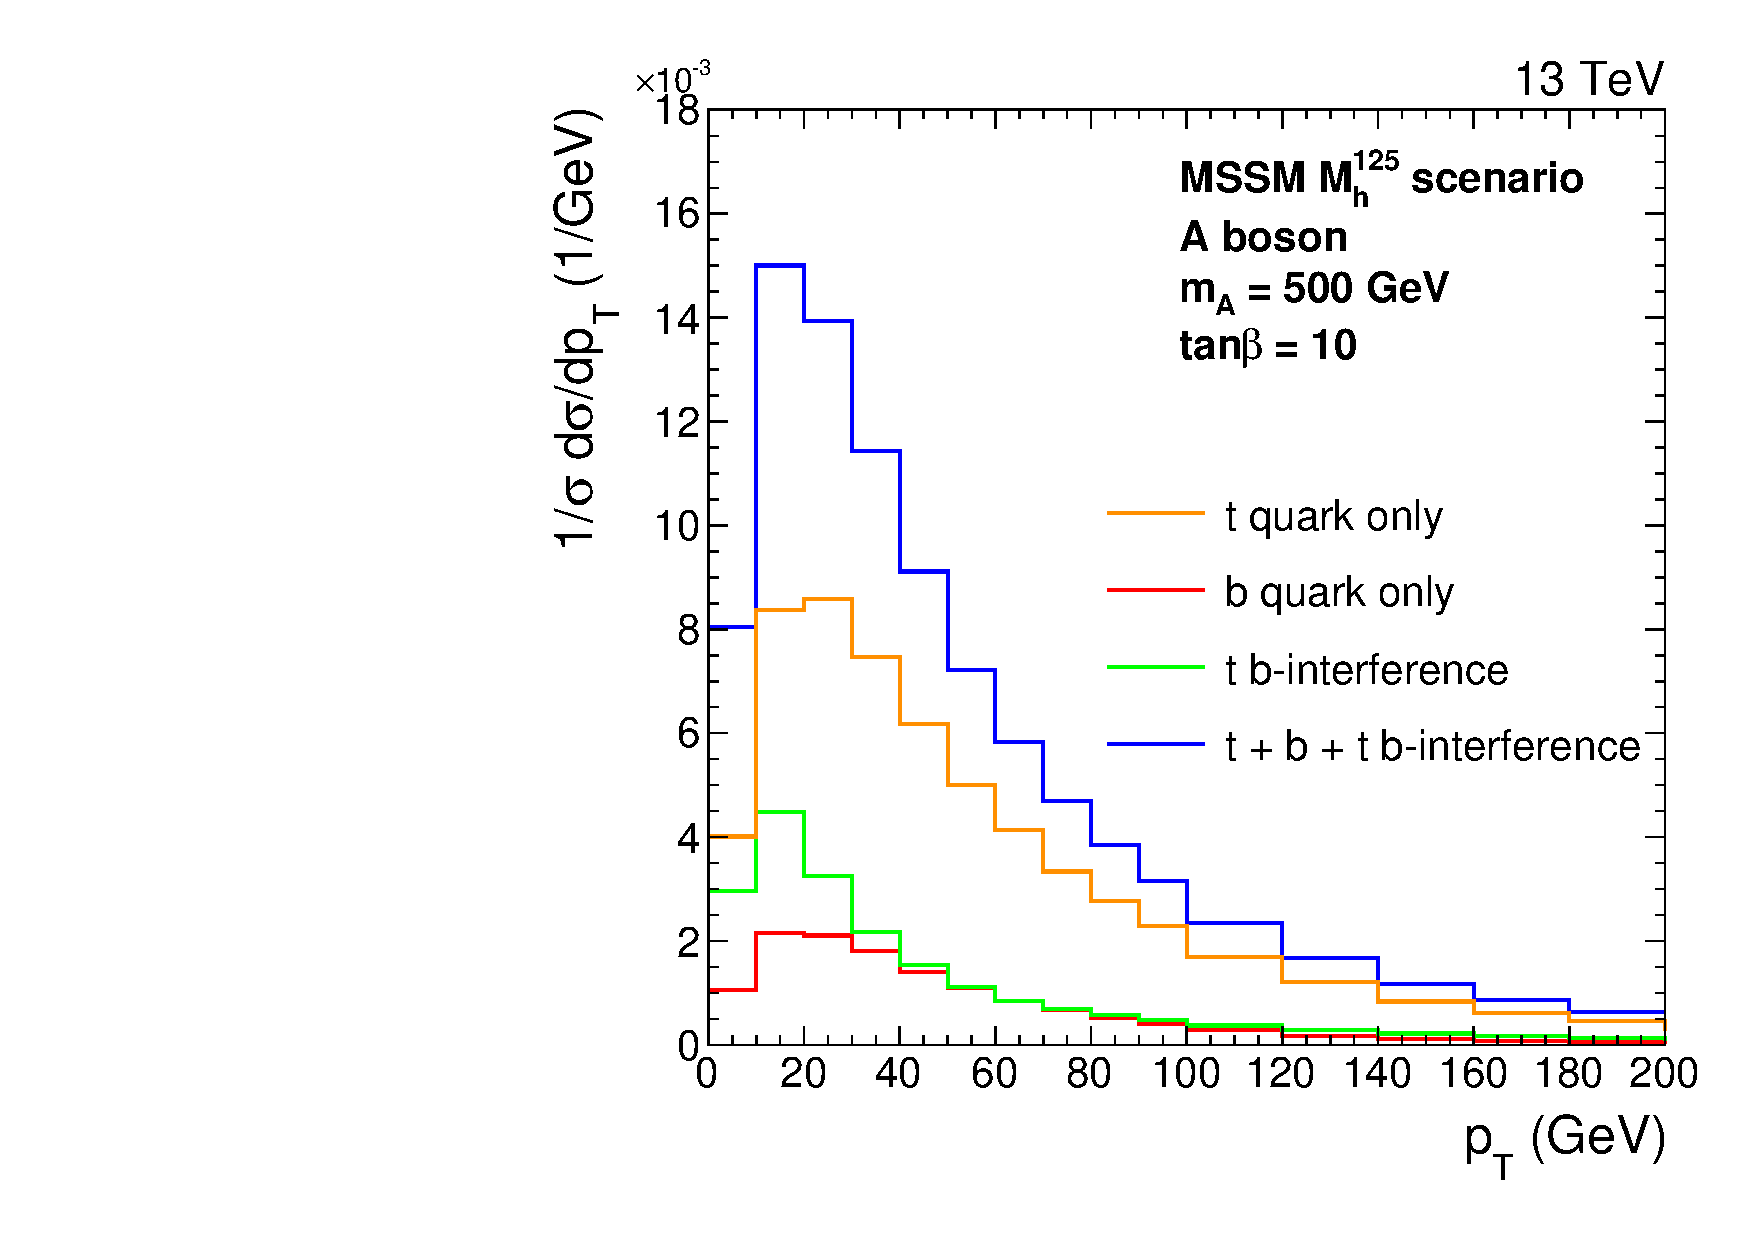
\includegraphics[width=0.5\textwidth]{Figures/pT_reweighting_plot_A10.pdf}}
    \subfloat[]{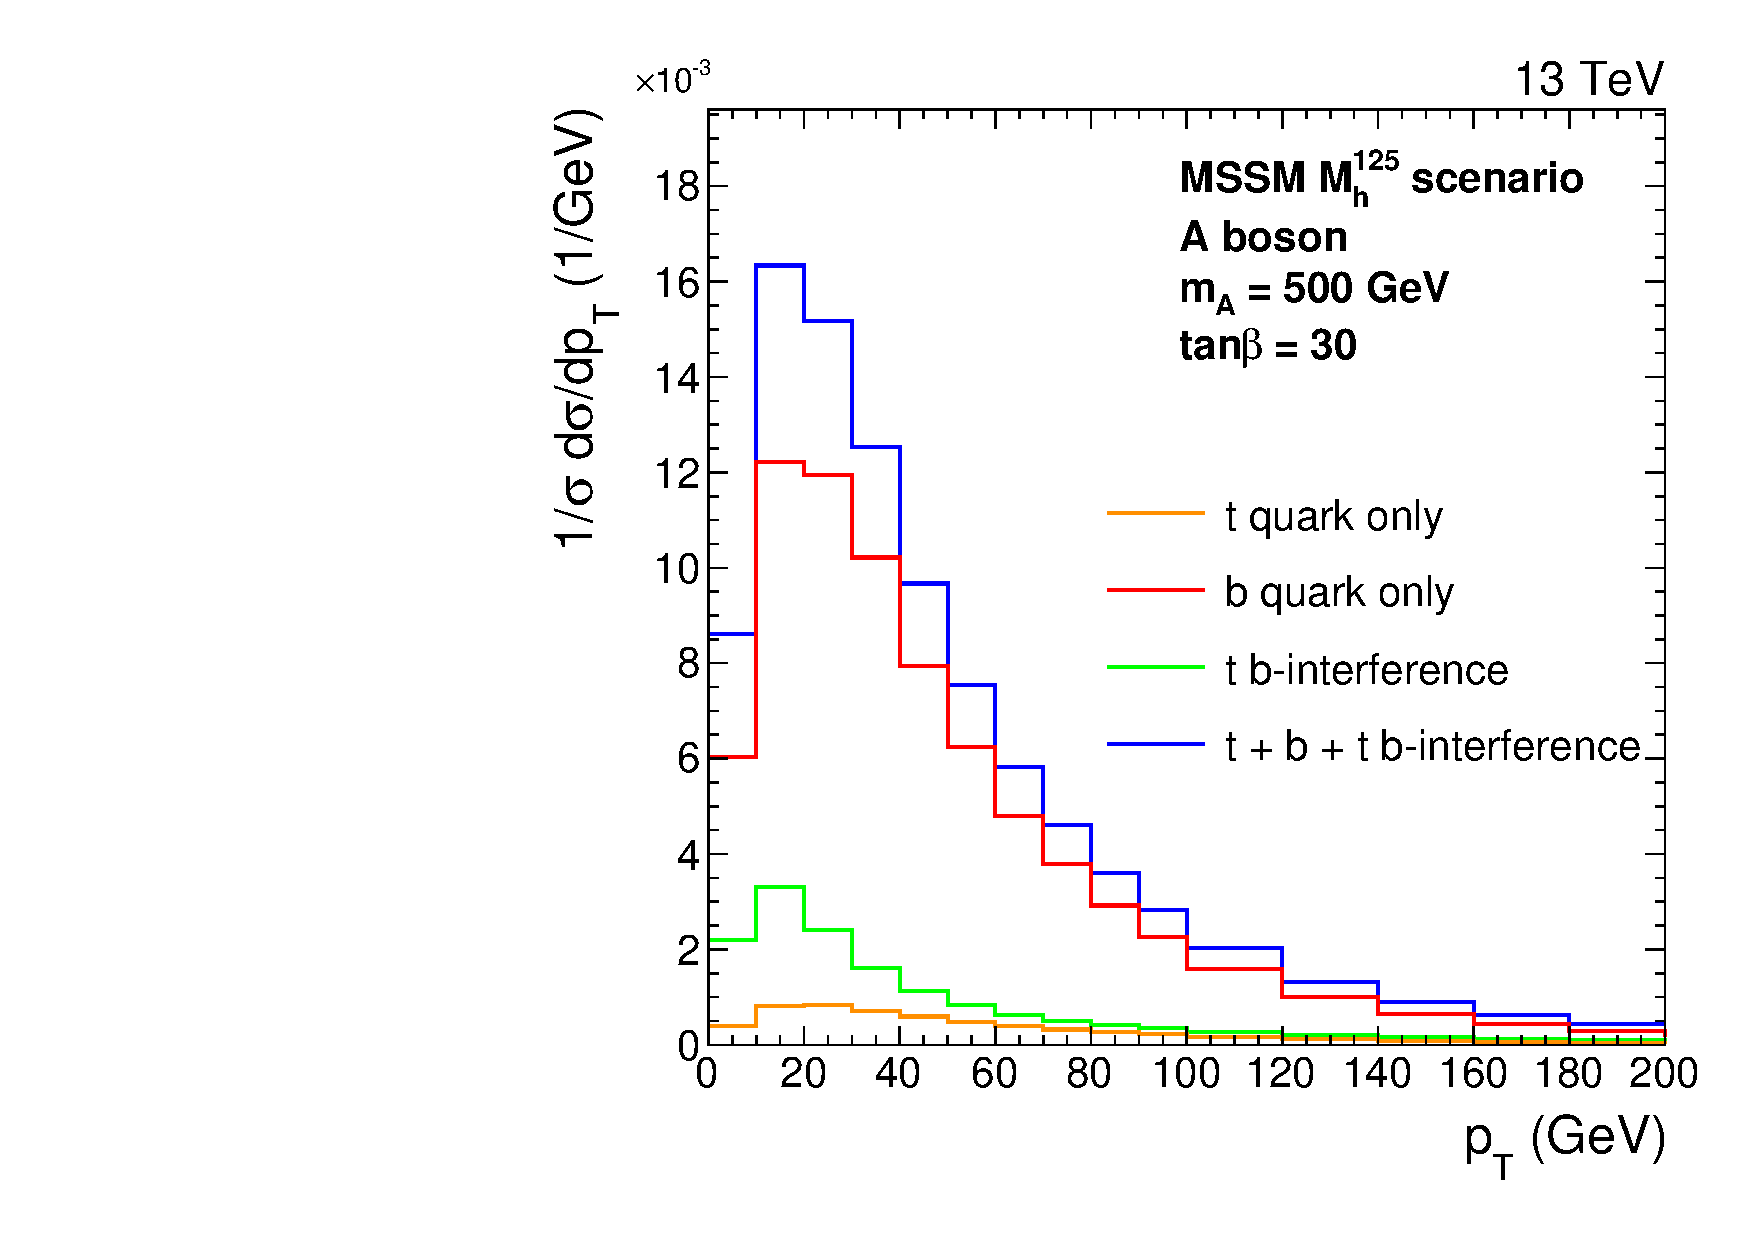
\includegraphics[width=0.5\textwidth]{Figures/pT_reweighting_plot_A30.pdf}} \\
    \subfloat[]{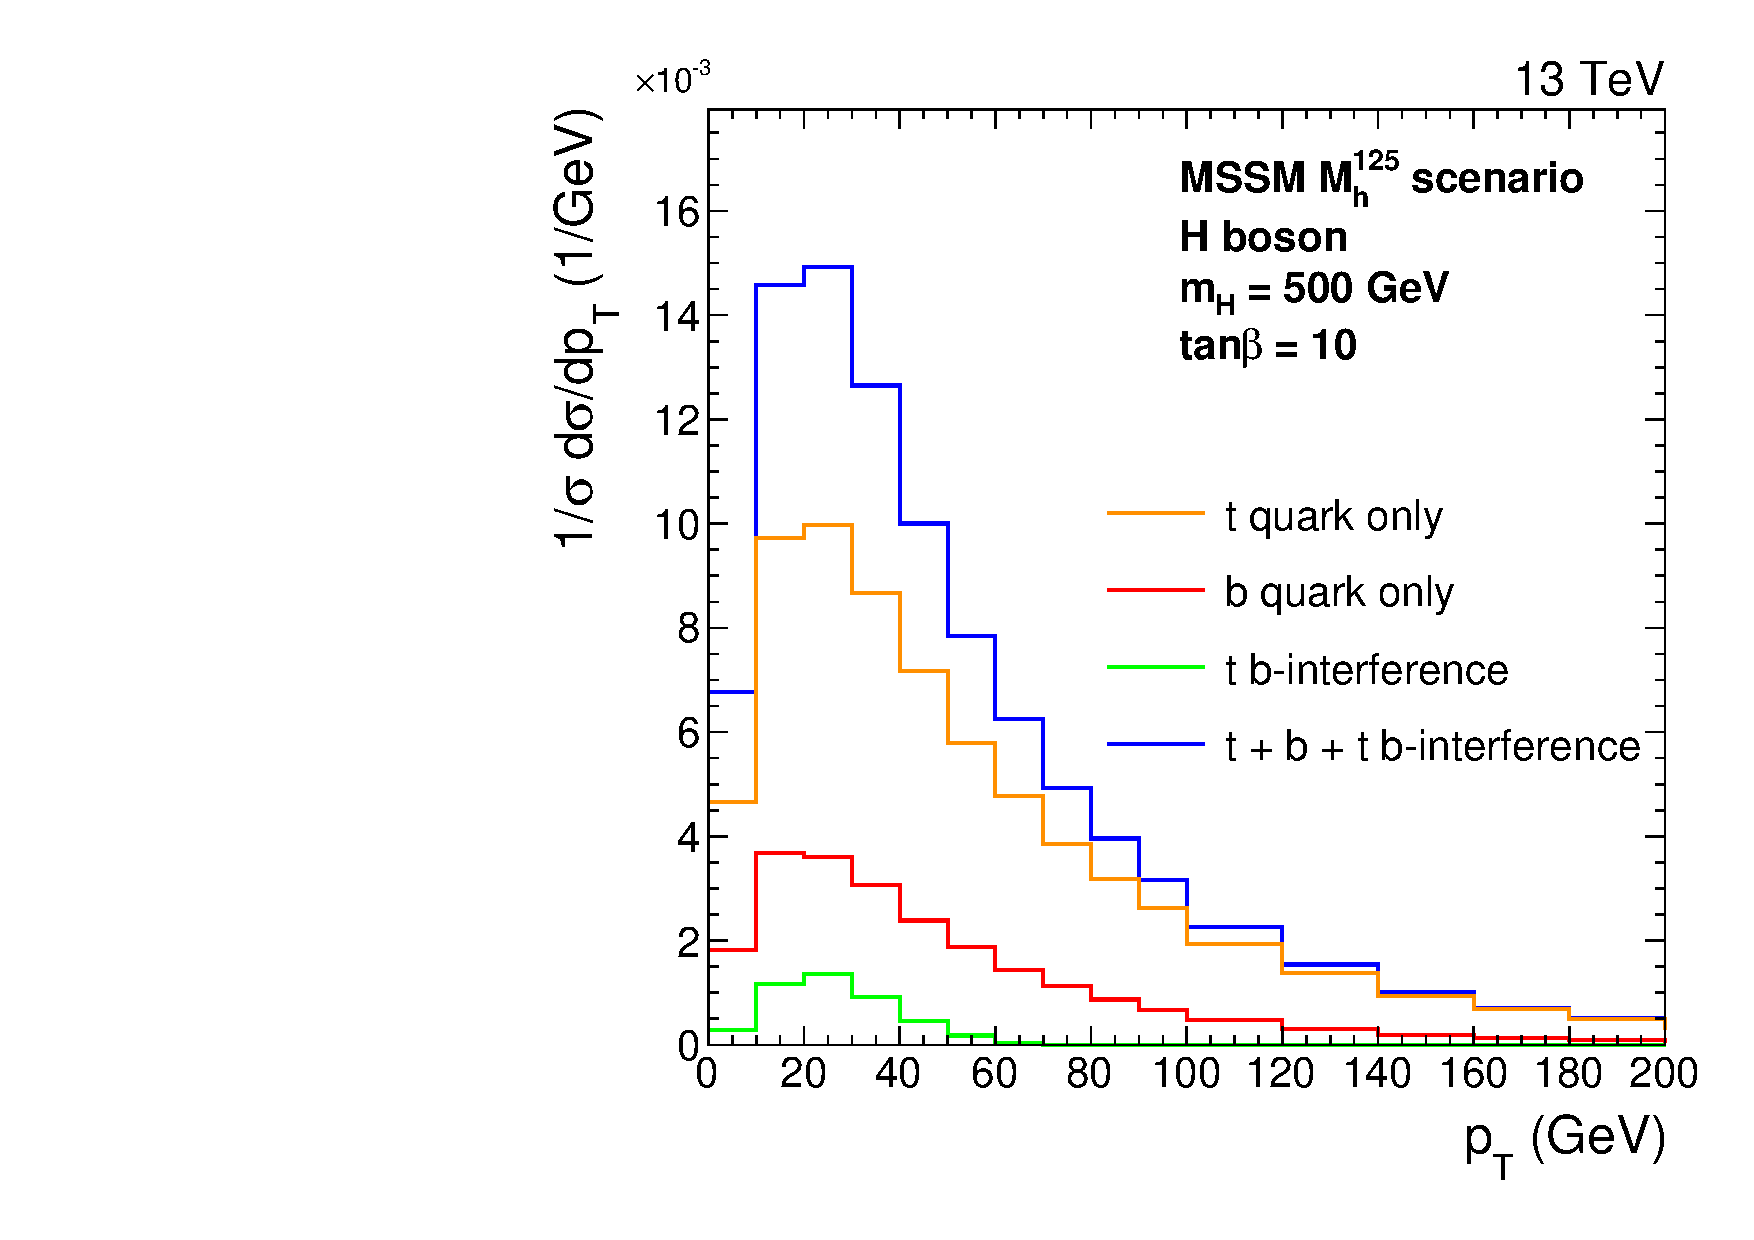
\includegraphics[width=0.5\textwidth]{Figures/pT_reweighting_plot_H10.pdf}}
    \subfloat[]{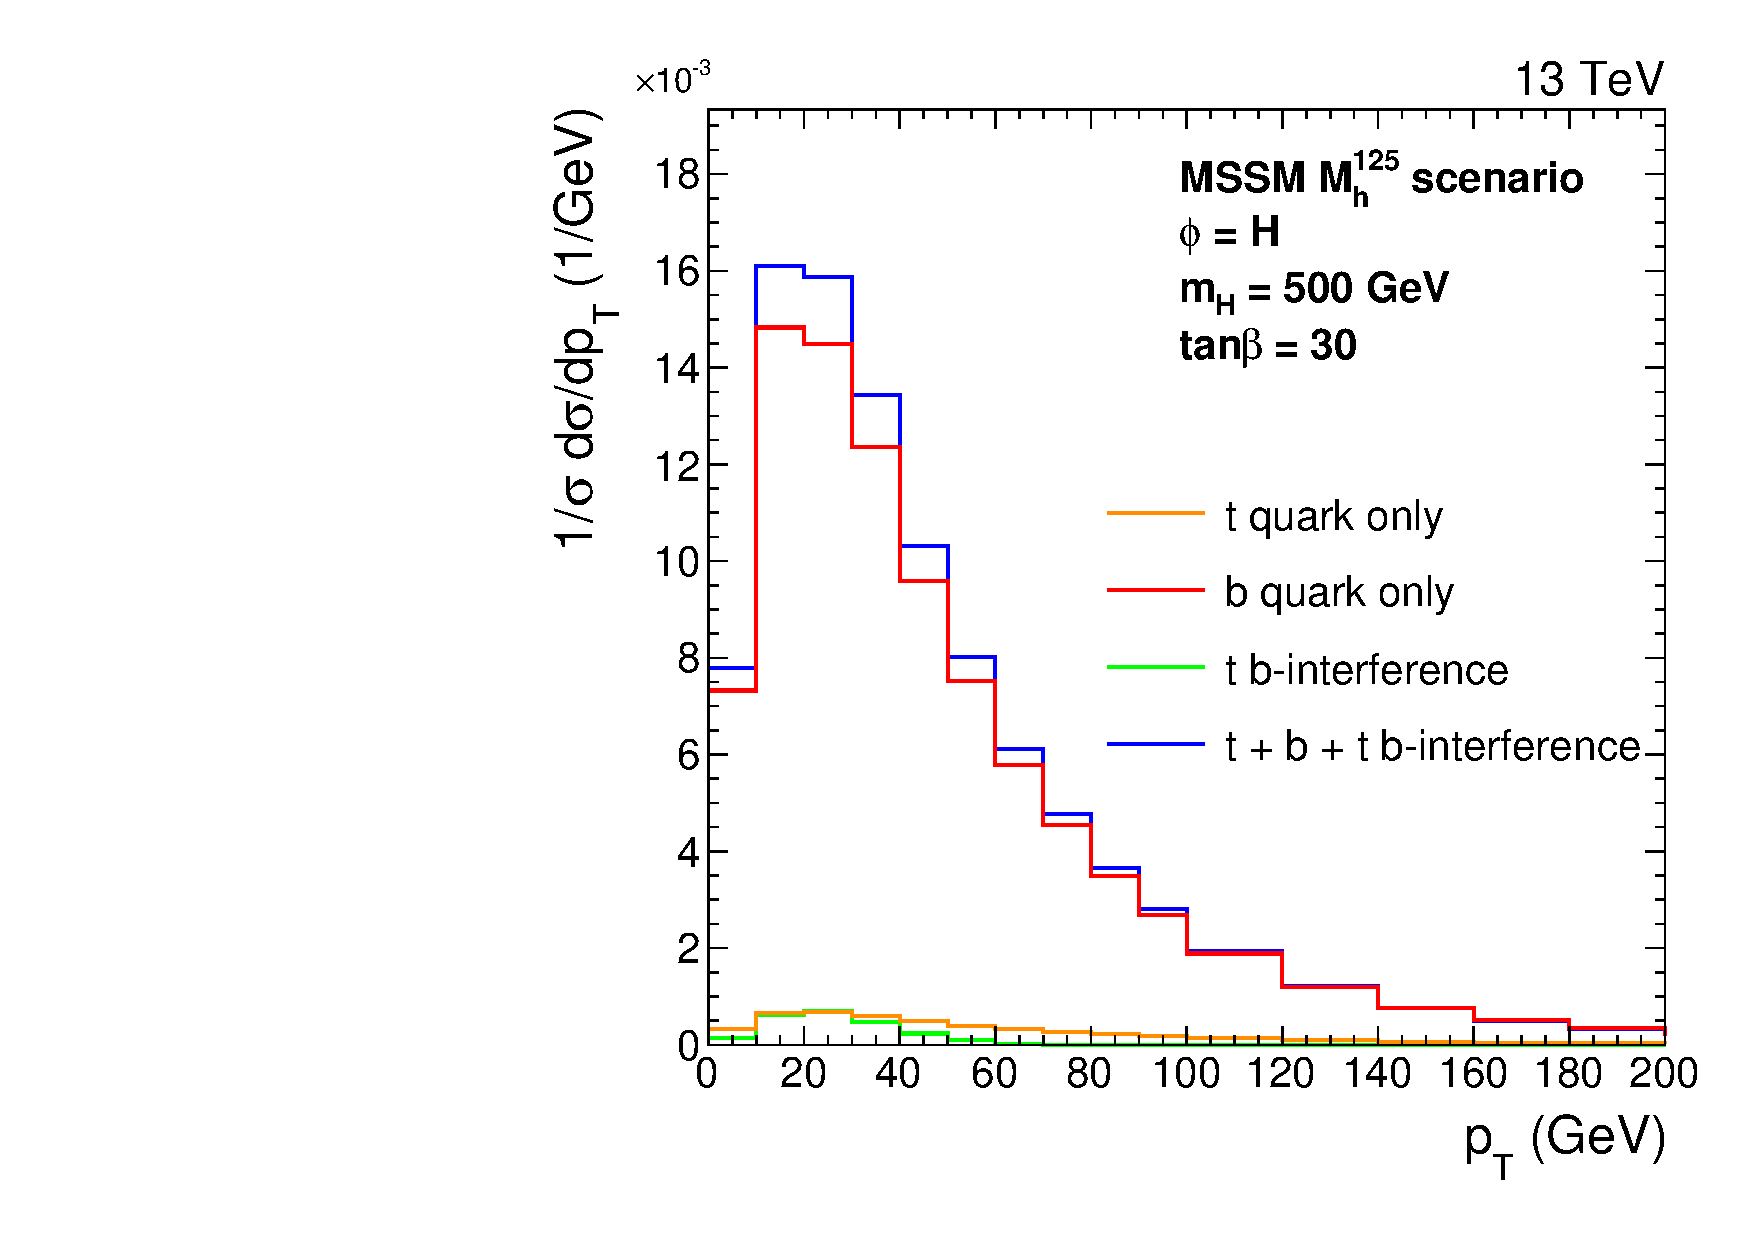
\includegraphics[width=0.5\textwidth]{Figures/pT_reweighting_plot_H30.pdf}} \\
\caption{$p_{T}$ density distributions of the A (top) and H (bottom) boson, with contributions to the gluon fusion loop displayed individually and summed. These are shown for $\tan\beta$ values of 10 (left) and 30 (right) where $m_{A} = 500$ GeV in the MSSM $M_{h}^{125}$ scenario.}
\label{fig:mssm_sig}
\end{figure}

Production in association with bottom quarks is simulated at NLO precision using the corresponding POWHEG 2.0 implementation in the four-flavour scheme.
All additional Higgs boson signal generation is performed using the parton distribution function (PDF) NNPDF3.1.
Tau lepton decay, parton showering and hadronisation are all modelled with the PYTHIA event generator where the PU profile is matched to data.
All events generated are passed through a GEANT4-based simulation of the CMS detector and reconstructed in the same way as data. \\

The model dependent search for the MSSM also looks to find differences from the observed SM Higgs boson and the predicted MSSM SM-like Higgs boson.
In each MSSM benchmark scenario, an uncertainty of $\pm 3$ GeV is given on the prediction for the SM Higgs boson mass.
This uncertainty is to reflect the contribution from any unknown higher-order corrections.
The value of the mass is allowed to vary within this window, however the Yukawa couplings are rescaled the observed mass.

\subsection{Vector Leptoquarks}
\label{sec:vlq}

The best fit in the vector leptoquark phase space to the B anomalies yielded large bottom quark and tau lepton couplings to the $U_1$ particle.
The possible production modes of a $\tau^+\tau^-$ final state are shown in Figure~\ref{fig:leptoquark_feynman}.


\begin{figure}[H]
\centering
\begin{subfigure}[b]{0.3\textwidth}
\begin{tikzpicture}[scale=2]
  \begin{feynman}
    \vertex [label=left:$\bar{q}$] (a1) at (0,0);
    \vertex [label=left:$q$] (a2) at (0,1);
    \vertex (b1) at (1,0);
    \vertex (b2) at (1,1);
    \vertex [label=right:$U_{1}$] (b3) at (1,0.5);
    \vertex [label=right:$\tau^-$] (c1) at (2,0);
    \vertex [label=right:$\tau^+$] (c2) at (2,1);

    \diagram* {
      (b1) -- [fermion] (a1),
      (a2) -- [fermion] (b2),
      (b2) -- [boson] (b1),
      (c1) -- [fermion] (b1),
      (b2) -- [fermion] (c2),
    };
  \end{feynman}
\end{tikzpicture}
\caption{}
\end{subfigure} \\

\begin{subfigure}[b]{0.3\textwidth}
\begin{tikzpicture}[scale=2]
  \begin{feynman}
    \vertex [label=left:$g$] (a1) at (0,0);
    \vertex [label=left:$g$] (a2) at (0,1);
    \vertex (b1) at (0.7,0.5);
    \vertex (b2) at (1.2,0.5);
    \vertex (c1) at (1.7,0.1);
    \vertex (c2) at (1.7,0.9);
    \vertex [label=$U_{1}$] (c1t) at (1.4,-0.05);
    \vertex [label=$U_{1}$] (c2t) at (1.4,0.72);
    \vertex [label=right:$\tau^+$] (d1) at (2.2,1.2);
    \vertex [label=right:$q$] (d2) at (2.2,0.6);
    \vertex [label=right:$\tau^-$] (d3) at (2.2,0.4);
    \vertex [label=right:$\bar{q}$] (d4) at (2.2,-0.2);
    
    \diagram* {
      (a1) -- [gluon] (b1),
      (a2) -- [gluon] (b1),
      (b1) -- [gluon] (b2),
      (b2) -- [scalar] (c1),
      (b2) -- [scalar] (c2),
      (d1) -- [fermion] (c2),
      (c2) -- [fermion] (d2),
      (c1) -- [fermion] (d3),
      (d4) -- [fermion] (c1),
    };
  \end{feynman}
\end{tikzpicture}
\caption{}
\end{subfigure}
\hspace{2cm}
\begin{subfigure}[b]{0.3\textwidth}
\begin{tikzpicture}[scale=2]
  \begin{feynman}
    \vertex [label=left:$g$] (a1) at (0,0);
    \vertex [label=left:$q$] (a2) at (0,1);
    \vertex (b1) at (0.7,0.5);
    \vertex [label=below:$q$] (bt) at (0.95,0.45);
    \vertex (b2) at (1.2,0.5);
    \vertex [label=right:$\tau^-$] (c1) at (2,0);
    \vertex (c2) at (1.7,0.9);
    \vertex [label=$U_{1}$] (c2t) at (1.4,0.72);
    \vertex [label=right:$\tau^+$] (d1) at (2.2,1.2);
    \vertex [label=right:$q$] (d2) at (2.2,0.6);

   
    \diagram* {
      (a1) -- [gluon] (b1),
      (a2) -- [fermion] (b1),
      (b1) -- [fermion] (b2),
      (b2) -- [fermion] (c1),
      (b2) -- [scalar] (c2),
      (d1) -- [fermion] (c2),
      (c2) -- [fermion] (d2),
    };
  \end{feynman}
\end{tikzpicture}
\caption{}
\end{subfigure}

\caption{Feynman diagrams showing the contribution from $U_1$ vector leptoquarks to the final state with a pair of oppositely charged tau leptons. Diagram (a) shows t-channel, (b) pair and (c) single production of a vector leptoquark.}
\label{fig:leptoquark_feynman}
\end{figure}

Pair and single production of a vector leptoquark is dependent on its strong coupling, which is highly model dependent.
For large mass, $m_U$, the probability of producing an on-shell $U_1$ singlet or pair is heavily suppressed due to the momentum of the initial partons.
These production processes are not discussed further in this search.
Further studies have been used to search for single and pair production at the CMS experiment and no statistically significance derivation was observed. \\

The t-channel process contain two vertices with a $U_1$ vector leptoquark, a quark and a tau lepton, and hence the cross section will scale with $g_{U}^4$.
From the best fit to B anomalies this vertex will be dominated by the b quark and hence the initial state will be mostly from $b\bar{b}$, with sub-dominant contributions from $b\bar{s}$, $s\bar{b}$ and $s\bar{s}$.
Although there are no additional b quarks in the final state in the LO process, initial state radiation can lead to additional b quarks in the final state.
In this search the two scenarios discussed in Section~\ref{sec:introduction} are considered.
The only non negligible parameter for $\tau^{+}\tau^{-}$ final states from the fit in the $m_{U}$-$g_{U}$ phase space is the $\beta_{L}^{s\tau}$ parameter.
This is set to the best fit value. \\

The signal process of the $U_1$ t-channel exchange is simulated in the five-flavour scheme (5FS) at LO precision using the \MGvATNLO event generator, v2.6.5.
Events are generated with one or fewer outgoing partons from the matrix element and the MLM prescription is then used for matching, with a scale set to 40 GeV.
Negligible dependence of the $U_1$ decay width ($\Lambda$) is observed, for simulation this is chosen to approximately match the value predicted by the B anomaly fit.
Samples with a mass between 1 and 5 TeV at $g_U = 1$ are generated. \\

The interference between the $U_1$ signal and $Z/\gamma^* \rightarrow \tau\tau$ production was checked.
A large destructive affect is observed, with the magnitude dependent on $g_{U}$.
To account for this, separate samples are produced for this interference, generated in the same way as the t-channel exchange.
The interference samples are then split into two with a di-tau mass split in order to have a sufficient number of events in the high di-tau mass regions.
The cross section of these interference samples scale with $g_{U}^2$. 
Examples of the generator level di-tau mass distributions are shown in Figure~\ref{fig:vlq_signal}. \\

\begin{figure}[!hbtp]
\centering
    \subfloat[]{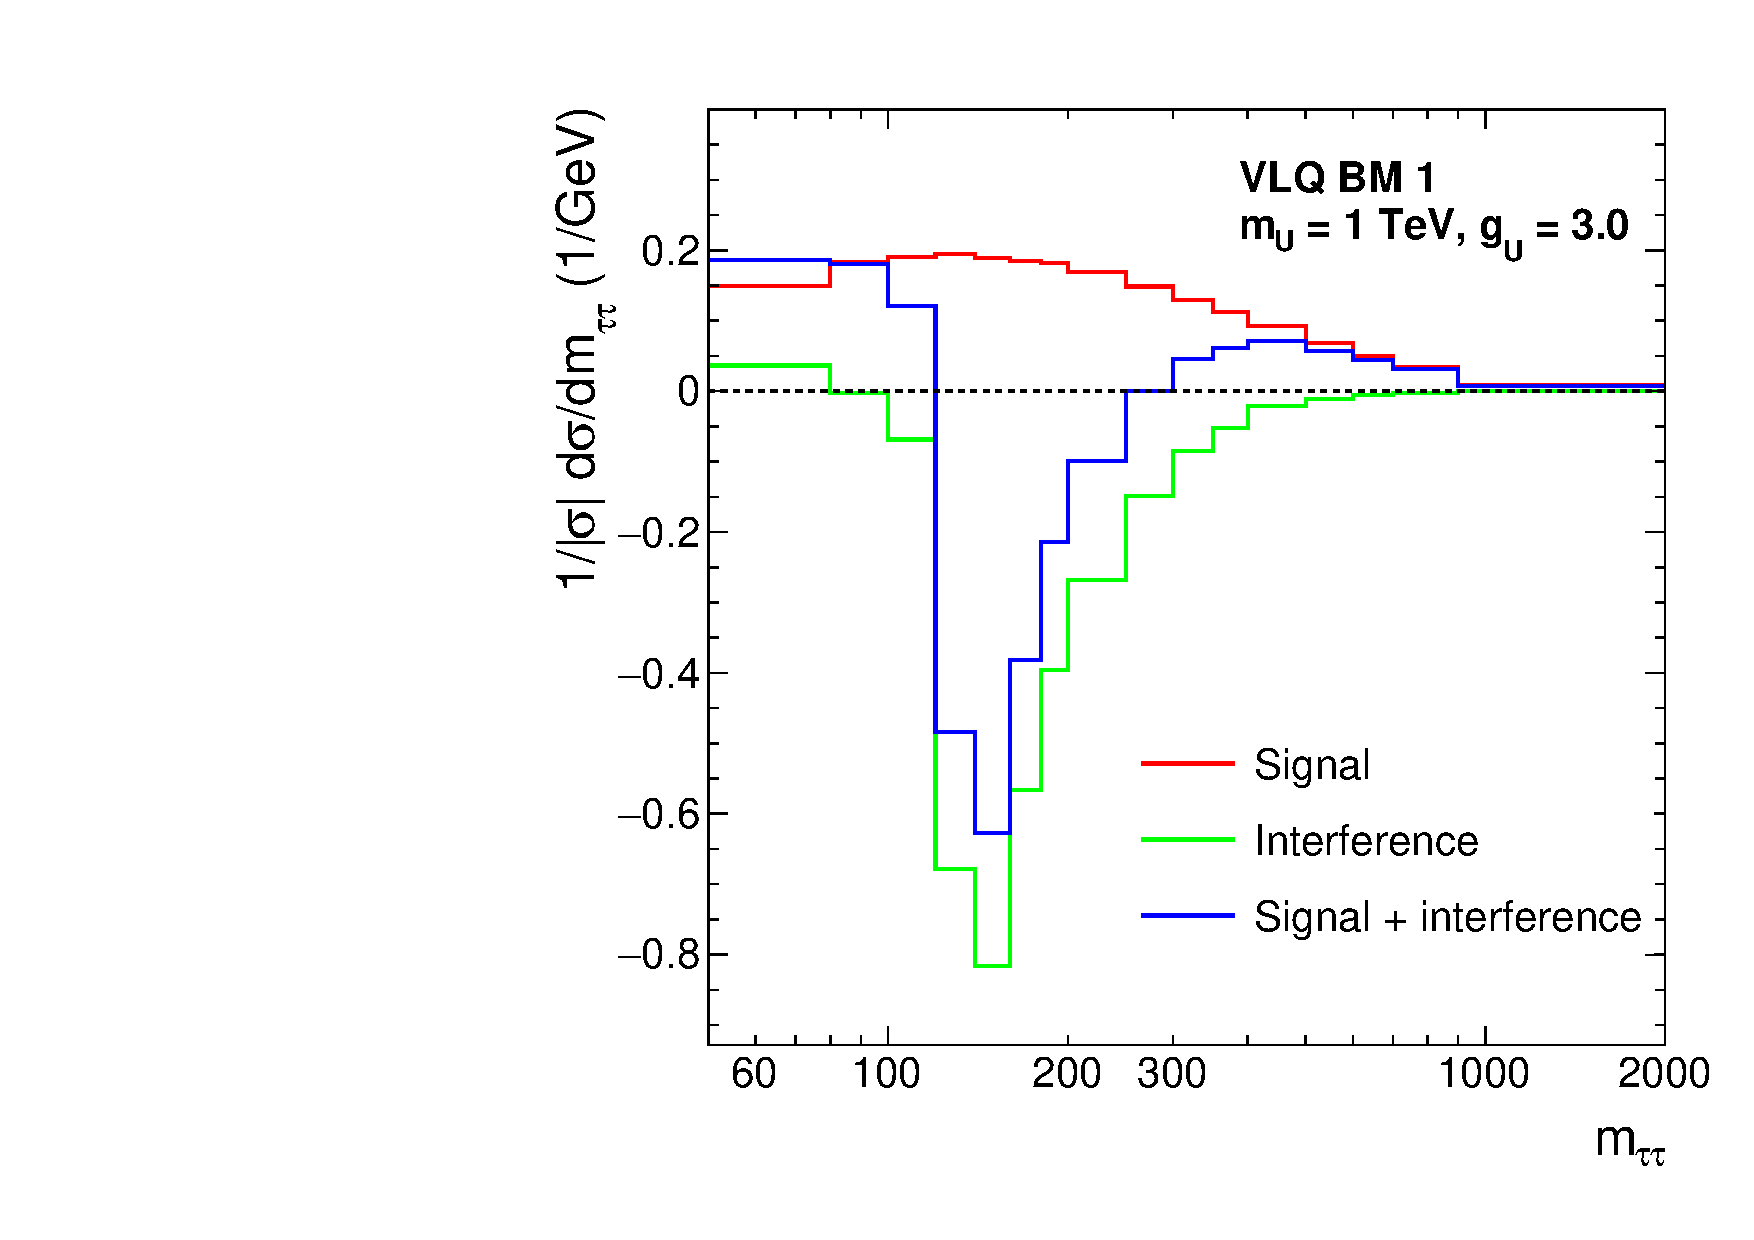
\includegraphics[width=0.5\textwidth]{Figures/vlq_signal_plot_gU3.pdf}}
    \subfloat[]{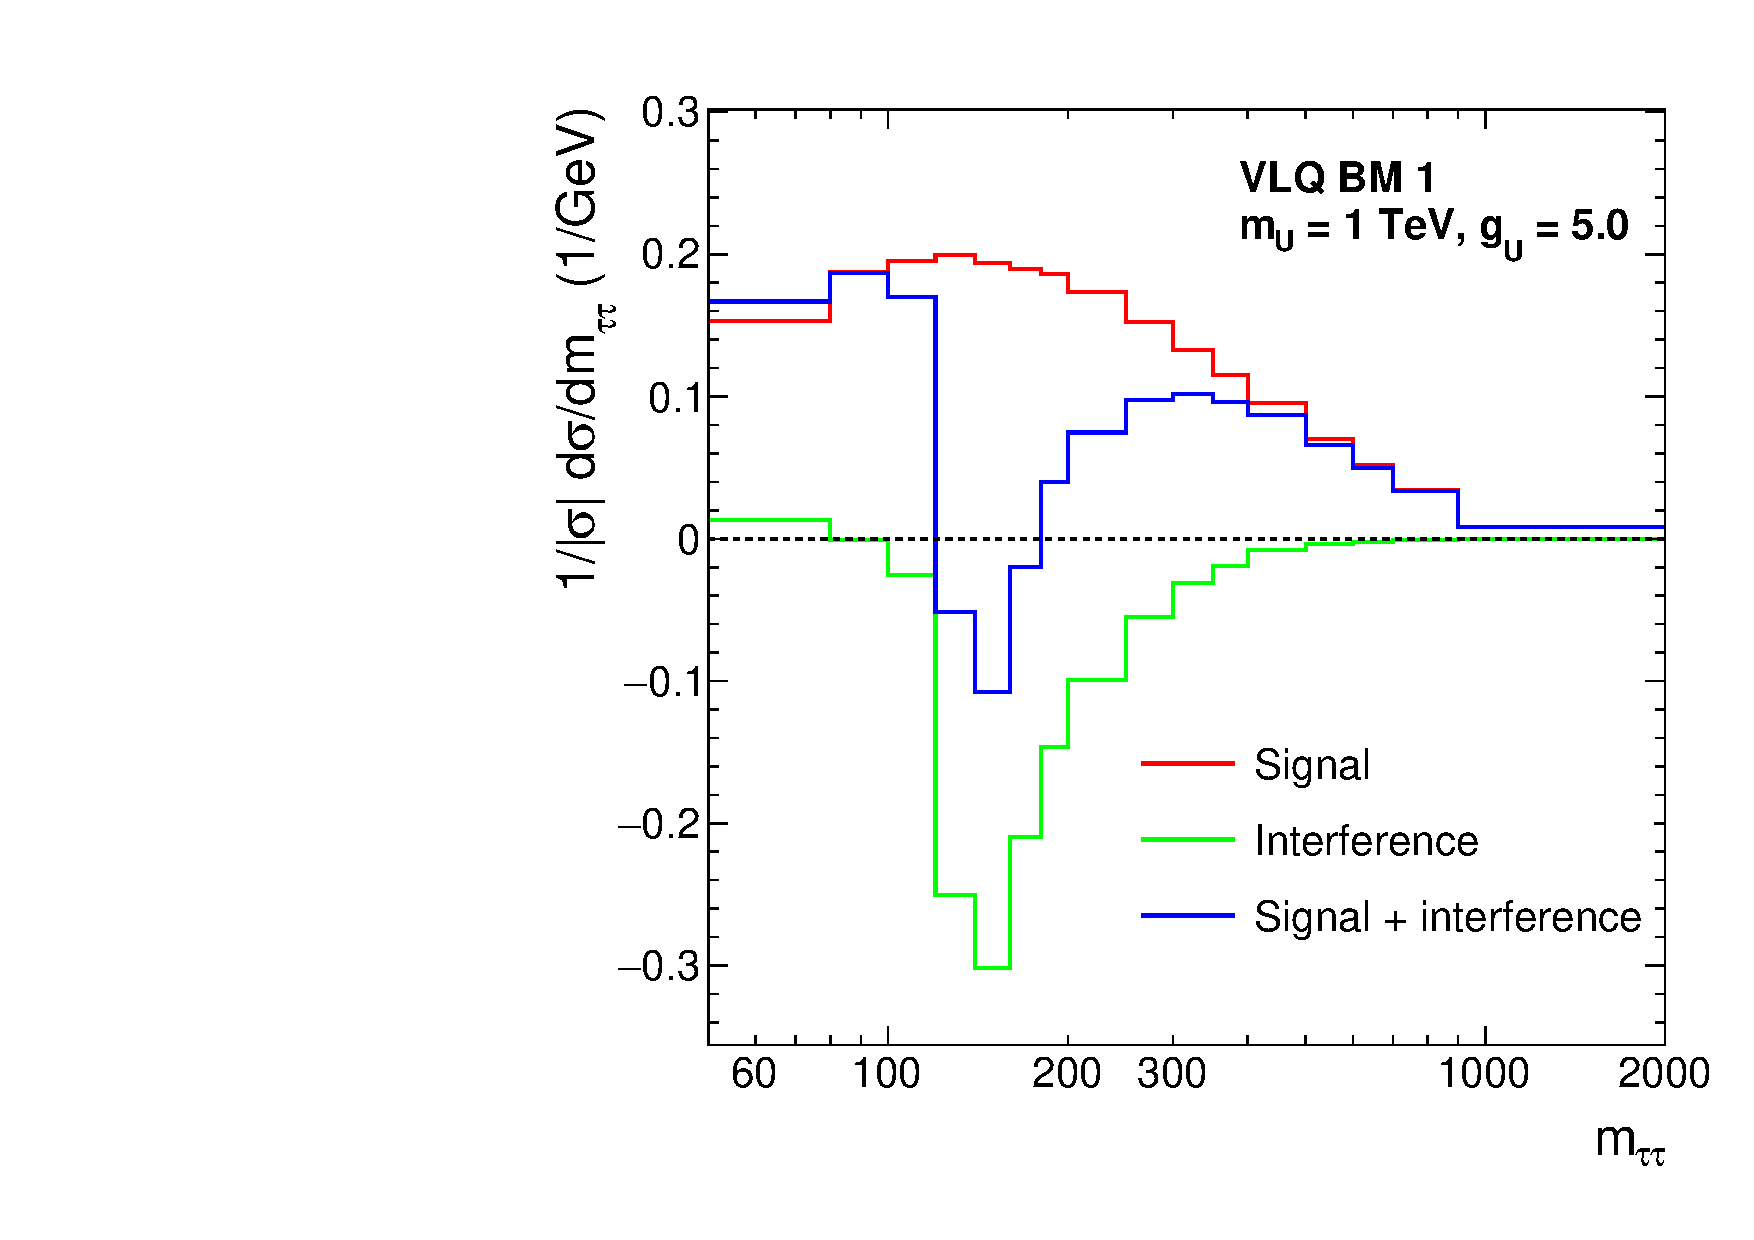
\includegraphics[width=0.5\textwidth]{Figures/vlq_signal_plot_gU5.pdf}}
\caption{The generator level $m_{\tau\tau}$ density distributions of the t-channel vector leptoquark signal and the interference with Drell-Yan. This is shown in the VLQ BM 1 scenario for a leptoquark of mass 1 TeV for coupling strengths of $g_{U}=3$ (a) and $g_{U}=5$ (b).}
\label{fig:vlq_signal}
\end{figure}

The t-channel signal produces a broad distribution in $m_{\tau\tau}$ due to its non-resonant nature.
The interference is mostly a destructive effect (except for at small $m_{\tau\tau}$), with the yield becoming less negative at higher $m_{\tau\tau}$.
The interference peaks negatively between 100 and 200 GeV and in this region the combined yield can be negative.
Due to the difference in scaling of the two effects, at small $g_{U}$ the interference is more dominant than the signal and hence the yield of the combined result is reduced.

\newpage
\section{Event Selection}

The possible decays of two tau leptons and their branching fractions, where the tau decay is grouped into three categories e, $\mu$ and $\tau_h$ as defined in Section~\ref{sec:object_reconstruction}, are shown in Table~\ref{tab:ditau_br}. 
For this search the four largest branching fraction channels used: $\tauhtauh$, $\etauh$, $\mutauh$ and $e\mu$.
This accounts for approximately 94\% of di-tau events.
The two same lepton channels are neglected due to small branching ratio and the dominating $Z\rightarrow ee$ and $Z\rightarrow \mu\mu$ backgrounds. \\

\begin{table}[!hbtp]
    \centering
    \begin{tabular}{|c|c|}
         \hline
         Channel & Branching Fraction  \\
         \hline
         \hline
         $\tauhtauh$ & 42.0\% \\
         $\etauh$ & 23.1\% \\
         $\mutauh$ & 22.6\% \\
         $\emu$ & 6.2\% \\
         $e e$ & 3.2\% \\
         $\mu \mu$ & 3.0\% \\
         \hline
    \end{tabular}
    \caption{Branching fractions of the decays of two tau leptons.}
    \label{tab:ditau_br}
\end{table}

\subsection{Trigger Requirements}

In the four final state pairs a number of different online trigger requirements are needed.
In the $\tauhtauh$ channel, two possible triggers are available: the double-$\tauh$ and single-$\tauh$ triggers.
The single-$\tauh$ trigger has a high $\pT$ threshold at 120 (180) GeV for events recorded in 2016 (2017-2018), whilst the double-$\tauh$ has a $\pT$ threshold at 40 GeV.
Therefore, the double-$\tauh$ trigger is used individually where the $\tauh$ has $\pT$ is below the single-$\tauh$ threshold and the union of single-$\tauh$ and double-$\tauh$ triggered events are taken above the threshold. \\

In the $\etauh$ and $\mutauh$ channels, there are three possible triggers available: the single-e/$\mu$, single-$\tauh$ and the e/$\mu$-$\tauh$ cross-trigger.
The cross-trigger is used for events where the light lepton has $\pT$ between the thresholds for the cross-trigger and single-$e/\mu$ shown in Table~\ref{tab:trig_thresholds}.
The light lepton used in the cross-trigger is required to be in the central barrel of the detector within $|\eta| < 2.1$.
Above these light lepton $\pT$ thresholds the single-$e/\mu$ trigger is used, where here it is required that the $\tauh$ has $\pT >$ 30 GeV.
At $\tauh$ $\pT$ above the single-$\tauh$ thresholds, the single-$\tauh$ trigger is used in combination with the single-$e/\mu$ trigger. \\

\begin{table}[hbtp]
  \centering
  \begin{tabular}{|c||c|c|c|c|}
    \hline
    Year/ Trigger   & $\etauh$ cross-trigger & single-$e$ & $\mutauh$ cross-trigger & single-$\mu$ \\
    \hline
    \hline
    2016 & 23                    & 26         & 20                     & 23           \\
    2017 & 25                    & 28         & 20                     & 25           \\
    2018 & 25                    & 33         & 21                     & 25           \\
    \hline        
  \end{tabular}
  \caption{Lower trigger light lepton thesholds $\pT$ in GeV for the $\etauh$ and $\mutauh$ channels.}
  \label{tab:trig_thresholds}  
\end{table}

In the $\emu$ channel, there are three possible triggers available: the single-$e$, single-$\mu$ and the e-$\mu$ cross-trigger.
However, only the cross-trigger is used in this analysis, due to the larger efficiencies of correctly selecting light leptons.
The e and $\mu$ are required to have $\pT >$ 15 GeV and $|\eta| < 2.4$.

\subsection{Offline Requirements}

All offline selections stated are in addition the object selection discussed in Section~\ref{sec:object_reconstruction}.
In this analysis, hadronic tau candidates are required to pass the \texttt{Medium} $D_{\text{jet}}^{\text{WP}}$.
$D_{e}^{\text{WP}}$ and $D_{\mu}^{\text{WP}}$ are dependent on the channel.
The \texttt{VVLoose}, \texttt{Tight}, \texttt{VVLoose} $D_{e}^{\text{WP}}$ and the \texttt{VLoose}, \texttt{VLoose} and \texttt{Tight} $D_{\mu}^{\text{WP}}$ are used in the $\tauhtauh$, $\etauh$ and $\mutauh$ channels respectively.
The tighter working point for the same light lepton discrimination as tagged in the event is used to remove light leptons faking hadronic taus from the $Z \rightarrow ll$ process.
The light lepton isolation requirement is $\Irel^{e/\mu} < 0.15$ except for in the $\emu$ channel where the muon is required to have $\Irel^{\mu} < 0.2$. \\

The selected $\tau$ lepton decay candidates are required to have opposite charge and to be separated by more than $\Delta R$ > 0.5 in all channels except $\emu$ where $\Delta R$ > 0.3.
In events where the numbers of an object in the event is greater than the required number of objects in the $\tau\tau$ decay channel, the objects are sorted by the maximum $D_{\text{jet}}^{\text{score}}$ if $\tau_h$ or minimum $\Irel$ if a light lepton and the leading objects are chosen.
In order to maintain orthogonality between channels, events with additional light leptons passing looser selections than the nominal requirements, are rejected from the selection.
The looser selections help to suppress the $Z \rightarrow ll$ background process further. \\

In the $\etauh$ and $\mutauh$ channels, a cut is placed at 70 GeV on the transverse mass between the light lepton $\pTvec$ and the missing $\pTvec$, where the transverse momentum is defined as,
\begin{equation}
m_{\text{T}}(\pTvec^{\hspace{2pt}i},\pTvec^{\hspace{2pt}j}) = \sqrt{2\pT^{i}\pT^{j}(1-\cos\Delta\phi)},
\label{eqn:mt}
\end{equation}
where $\Delta\phi$ to the azimuthal angle between $\pTvec^{\hspace{2pt}i}$ and $\pTvec^{\hspace{2pt}j}$.
The variable is used to remove W + jets background events, where a jet fakes a hadronic tau and the MET and light lepton from the W decay are aligned and hence the event has a large $m_{T}(\pTvec^{\hspace{2pt}e/\mu},\pTvec^{\hspace{2pt}\text{MET}})$.

In the $\emu$ channel an additional cut is placed on a variable named $D_{\zeta}$, which is defined as,
\begin{equation}
D_\zeta = p_\zeta^\text{miss} - 0.85 p_\zeta^\text{vis};\qquad
p_\zeta^\text{miss} = \pTvec^{\hspace{2pt}\text{miss}} \cdot \hat{\zeta};\qquad
p_\zeta^\text{vis} = (\pTvec^{\hspace{2pt}e} + \pTvec^{\hspace{2pt}\mu}) \cdot \hat{\zeta}
\label{eqn:Dzeta_def}
\end{equation}
where $\pTvec^{\hspace{2pt}e/\mu}$ corresponds to the transverse momentum vector of the electron or muon and $\hat{\zeta}$ to the bisectional direction between the electron and the muon in the transverse plane~\cite{CDFPzeta}.
A diagram of the inputs is shown Figure~\ref{fig:dzeta_diagram}. \\
\begin{figure}[!hbtp]
\centering
    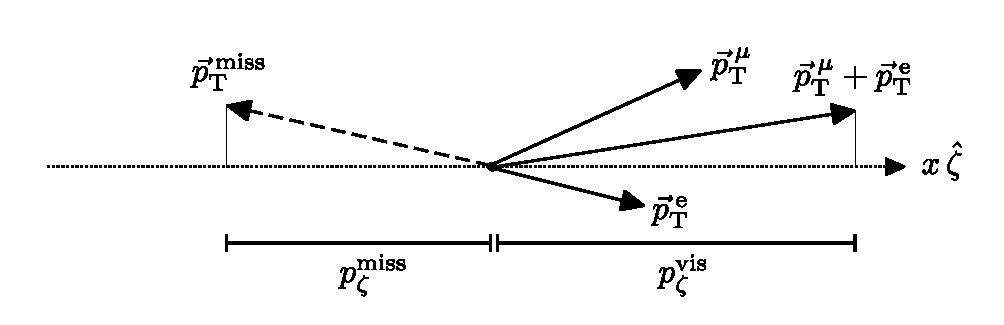
\includegraphics[width=1.0\textwidth]{Figures/dzeta_diagram.pdf}
\caption{Diagram of inputs to the $D_\zeta$ variable.}
\label{fig:dzeta_diagram}
\end{figure}

The linear combination is optimised for genuine di-tau events to peak around $D_{\zeta} = 0$ GeV. 
It is motivated by the expectation that in di-tau decays from a resonance, the visible and missing (from tau neutrinos) momentums are roughly aligned and of similar magnitudes.
In W + jets and $\ttbar$ events the directions of the visible and missing products are expected to be more randomly distributed and lead to a non-peaking $D_{\zeta}$.
Therefore only events with $D_\zeta >$ -35 GeV are considered for signal events.
No b tagged events with this cut are vetoed and b tagged events with this cut are used for a $\ttbar$ control region and discussed further in Section~\ref{sec:background_modelling}.

\newpage
\section{Search Optimisation}
\label{sec:search_optimisation}

The optimisation of the signal extraction depends on which of the three scenarios, set out at beginning of this section, is searched for.
The components of the optimisation are named the high mass, low mass and SM Higgs optimisation procedures.
For the model independent search (i) the high or low mass optimisation procedures are used depending on whether the mass of the resonance is greater or less than 250 GeV.
The search for the MSSM Higgs sector (ii) uses the high mass or the SM Higgs optimisation procedures depending on whether the reconstructed di-tau mass \cite{} is greater or less than 250 GeV.
Finally, the search for vector leptoquarks (iii) uses only the high mass optimisation procedure.
The procedures are discussed in detail below. \\

The high mass optimisation procedure follows what was done in Ref. \cite{}.
Firstly each category is split into categories with no b tagged and with one or more b tagged events.
This firstly helps target the additional Higgs boson production modes gluon fusion and b associated production respectively.
Secondly, the initial state radiation of a t-channel vector leptoquark signal dominated by initial states of b quarks, can lead to additional b jets in the final state.
The reduced backgrounds in b tagged events allows for a more sensitive vector leptoquark search in this category. \\

The $\etauh$ and $\mutauh$ channels are further subdivided into categories depending on the transverse mass between the light lepton and missing transverse momentum vectors as defined in Equation~\ref{eqn:mt}.
The corresponding categories are defined as:
\begin{itemize}
\item \texttt{Tight-$m_{\text{T}}$}: $m_{\text{T}}(\pTvec^{\hspace{2pt}e/\mu},\pTvec^{\hspace{2pt}\text{miss}}) < 40$ GeV;
\item \texttt{Loose-$m_{\text{T}}$}: $40 \leq m_{\text{T}}(\pTvec^{\hspace{2pt}e/\mu},\pTvec^{\hspace{2pt}\text{miss}}) < 70$ GeV.
\end{itemize}
The majority of the signal events fall within the \texttt{Tight-$m_{\text{T}}$} sub-category.
The \texttt{Loose-$m_{\text{T}}$} category is used improve the signal acceptance for resonant masses of $m_{\phi} > 700$ GeV.\\


In the $\emu$ channel, is also subdivided into three signal categories based of the cuts on the variable $D_{\zeta}$ as defined in Equation~\ref{eqn:Dzeta_def}.
The three categories are defined as:
\begin{itemize}
\item \texttt{Low-$D_\zeta$}: $-35 \leq D_\zeta < -10$ GeV;
\item \texttt{Medium-$D_\zeta$}: $-10 \leq D_\zeta [\GeV] <  30$ GeV;
\item \texttt{High-$D_\zeta$}: $D_\zeta [\GeV] \geq 30$ GeV.
\end{itemize}
By design, the majority of signal events are located in the \texttt{Medium-$D_\zeta$} sub-category.
The Low and High-$D_\zeta$ categories are used to catch the tail of the signal distributions.
A schematic of all high mass optimisation categories are shown in Figure ~\ref{fig:high_mass_categories}. \\

\begin{figure}[!hbtp]
\centering
    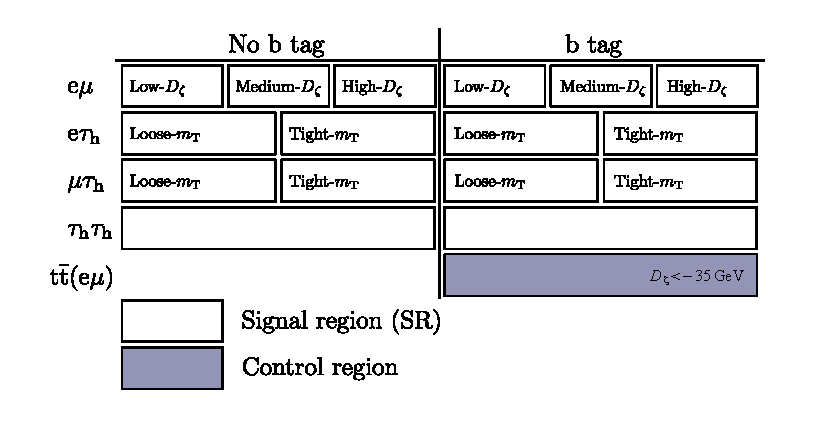
\includegraphics[width=1\textwidth]{Figures/high_mass_categories.pdf}
\caption{Overview of the categories used for the extraction of the signal in the high mass optimisation procedure.}
\label{fig:high_mass_categories}
\end{figure}

Once all category divisions have been applied, events are drawn in histograms based off a discriminating variable.
The discriminating variable used in this analysis is $m_{T}^{\text{tot}}$ and is defined below.
\begin{equation}
m_{T}^\text{tot} = \sqrt{m_{T}(\pTvec^{\hspace{2pt}\tau_1},\pTvec^{\hspace{2pt}\text{miss}})^2 +  m_{T}(\pTvec^{\hspace{2pt}\tau_2},\pTvec^{\hspace{2pt}\text{miss}})^2 + m_{T}(\pTvec^{\hspace{2pt}\tau_1},\pTvec^{\hspace{2pt}\tau_2})^2},
\label{eqn:mt_tot}
\end{equation}
where $\tau_1$ and $\tau_2$ refer to the visible products of the two tau leptons decays.
This variable provides excellent discriminating power between higher mass resonant signals compared to other non-peaking backgrounds whilst still maintaining some separation between signal masses.
It is also excellent at separating the high mass non-resonant di-tau signatures where a di-tau mass is unphysical for the signal, due to the use of the $\pT$s and in the variable.
For the t-channel signal with the mediator has high mass, no significant mass separation is expected in any variable.

The low mass optimisation procedure loosely follows the high mass procedure with a few key difference.
Firstly categories that are only sensitive to high mass signals are dropped.
This includes the Low-$D_\zeta$ and Loose-$m_{T}$ categories.
Each no b tag subcategory is further divided into four bins of reconstructed di-tau visible $\pT$ with bin edges: 0,50,100,200 and $\infty$.
This is not done in the b tag subcategories due to the lack of statistics in this region.
A schematic of the categories used in the low mass optimisation procedure is shown in Figure~\ref{fig:low_mass_categories}.

\begin{figure}[!hbtp]
\centering
    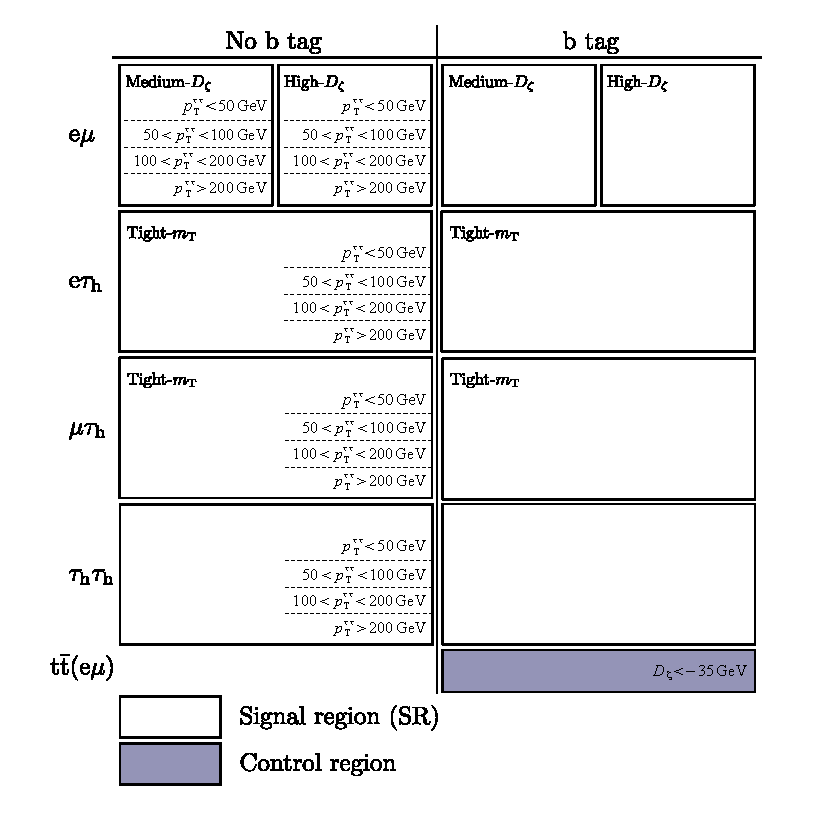
\includegraphics[width=1.0\textwidth]{Figures/low_mass_categories.pdf}
\caption{Overview of the categories used for the extraction of the signal in the low mass optimisation procedure.}
\label{fig:low_mass_categories}
\end{figure}

The final difference with the high mass optimisation procedure is the discriminator used, here the reconstructed di-tau mass is used.
This helps to separate signal events from the Z boson peak in this region.
Examples of the signal mass separations in the $\tauhtauh$ channel with the low and high mass discriminators are shown in Figure~\ref{fig:} \\

FIGURES OF DISTRIBUTIONS
VLQ AND INTERFERENCE
GGH AND BBH heavy
GGH AND BBH light \\

Finally the SM Higgs optimisation procedure is taken from the CMS SM $H \rightarrow \tau\tau$ analysis.
This was previously used for simplified template cross section measurements.
This uses a neural-network-based (NN) to obtain the most precise estimates from data of the SM Higgs produced via gluon fusion, vector boson fusion or vector boson associated production.
The NN based analysis introduces 26 categories, 8 of which are optimised to pull the out the Higgs boson signal.
Although the NN is trained specifically to target events with an SM-like Higgs boson, signal events with differing masses can also enter the NN categories.

\newpage
\section{Background Modelling Overview}
\label{sec:background_modelling}

The analysis considers several backgrounds including Drell-Yan, $\ttbar$, W+jets, QCD, di-boson, single-top, and electroweak W and Z bosons production.
These are split into a five categories:
\begin{enumerate}[i)]
  \item Events containing only genuine tau leptons.
  \item Events with a jet misidentified as a hadronic tau (jet$\rightarrow \tauh$) in the $\etauh$, $\mutauh$ or $\tauhtauh$ channels.
  \item Events with jets faking both light leptons (jet$\rightarrow l$) in the $\emu$ channel.
  \item Events from $\ttbar$ with a prompt light lepton ($e$ or $\mu$ not from a $\tau$ decay) and the other object (if there are not two prompt light lepton) is from a genuine tau leptons.
  \item Other events. This is a small contribution and hence why it is grouped.
  \begin{itemize}
    \item Non $\ttbar$ events with a prompt light lepton ($e$ or $\mu$ not from a $\tau$ decay) and the other object (if there are not two prompt light lepton) is from a genuine tau leptons.
    \item Events with a light lepton faking a hadronic tau and the other object (if there are not two light leptons faking a hadronic tau) are reconstructed as prompt light lepton or from genuine tau leptons. 
    \item Events with a jet faking a light lepton and the other object is from genuine tau leptons in the $\etauh$, $\mutauh$ or $\tauhtauh$ channels.
    \item Events with one jet faking a light lepton and the other object from a prompt light lepton in the $\emu$ channel.
   \end{itemize}
\end{enumerate}

Backgrounds from (i) consists of largely Z/$\gamma^* \rightarrow \tau\tau$ events but there are also smaller contributions from other processes. 
This background is modelled by a data-simulation hybrid method called the embedding method and this is described in detail in Section~\ref{sec:embedding}.
Group (ii) is dominated by QCD, W + jets and $\ttbar$ events with a jet$\rightarrow \tauh$ misidentification.
This is modelled from data by the fake factor method ($\FF$) and is explained in Section~\ref{sec:ff}.
Group (iii) is modelled from data to describe QCD multijet contribution to the background in the $\emu$ channel.
The method to obtain this background is described in Section~\ref{sec:qcd}.
The data driven background estimations for (i), (ii) and (iii) contribute >98\% of all expected background events in the $\tauhtauh$ channel, >90\% in $\etauh$ and $\mutauh$ channels and >50\% in the $\emu$ channel.
The final groups, (iv) and (v), are modelled with MC.
The $\ttbar$ process is separated due to its large contribution to the phase space where a b jet is required. \\

The W + jets and $Z\rightarrow ll$ processes are simulated at leading order (LO) using the \MGvATNLO 2.2.2 (2.4.2) event generator~\cite{Alwall:2011uj,Alwall:2014hca} for the simulation of the data taken in 2016 (2017--2018). 
To increase the number of simulated events in regions of high signal purity, supplementary samples are generated with up to four outgoing partons in the hard interaction. 
For diboson production, \MGvATNLO is used at next-to-LO (NLO) precision. 
In each case, the FxFx~\cite{Frederix:2012ps} (MLM~\cite{Alwall:2007fs})  prescription is used to match the NLO (LO) matrix element calculation with the parton shower model. 
For $\ttbar$~\cite{Alioli:2011as} and (t-channel) single top quark production~\cite{Frederix:2012dh}, samples are generated at NLO precision using \POWHEG 2.0~\cite{Nason:2004rx,Frixione:2007vw,Alioli:2010xd,Jezo2015aia}. 
The \POWHEG version 1.0 at NLO precision is used for single top quark production in association with a W boson (tw channel)~\cite{Re:2010bp}. 

When compared with data, W + jets, $Z\rightarrow ll$, $\ttbar$, and single top quark events in the tW channel are normalised to their cross sections at next-to-NLO (NNLO) precision~\cite{Melnikov:2006kv,Czakon:2011xx,Kidonakis:2013zqa}. 
Single top quark (t-channel) and diboson events are normalized to their cross sections at NLO precision or higher~\cite{Kidonakis:2013zqa,Campbell:2011bn,Gehrmann:2014fva}.

\newpage
\section{QCD Estimation in the $\emu$ Channel}
\label{sec:qcd}

The QCD model in the $\emu$ channel, that attempts to model events where two jets are misidentified as an election muon pair, is taken from data with same sign election muon pair with a transfer factor ($F_{T}$).
The transfer factor determines differences from the same sign to opposite sign region is calculated from a sideband region with an anti-isolated muon ($0.2 < \Irel^{\mu} < 0.5$).
$F_{T}$ is initially parameterised by the $\Delta R$ between the election and muon, and the number of jets in the event, however additional dependencies on the electron and muon $\pT$ enter via a correction. \\
Good agreement is observed in events with no b jets, for the discriminating variables discussed in Section~\ref{sec:sig_ext}, when applying $F_{T}$ onto same sign events compared to opposite sign events where both regions have an anti-isolated muon. 
However in events with b jets, an additional correction is needed.
This is determined to be ~0.75 (differs very slightly between data taking years).
As this correction is large, it is validated by switching the light lepton anti-isolation, so that the election is required to have $0.15 < \Irel^{e} < 0.5$.
Also events where both light leptons are anti-isolated are looked at.
The correction for b tagged events is equivalent in all three regions, and a global average of the three is taken for the final correction. \\

To understand the physical reason for the large difference in no b tag and b tag events in same sign and opposite pairs, studies were performed on simulated samples.
It was observed that the electron muon pair is usually produced from pairs of heavy quarks, $pp\rightarrow b\bar{b}$ ($c\bar{c}$).
If the two jets are initiated from the heavy quarks there is a large bias towards opposite sign jets due to the opposite signs of the quark anti-quark pair.
However if one of the heavy quarks is tagged as a b jet, another object has to be the jet initiator (a radiated gluon for example) and there is therefore no charge preference in the pair.
As $F_{T}$ is originally fit inclusively in numbers of b jets and the 0 bin is dominant, the correction over predicts the opposite sign to same sign ratio and so a large correction is needed as observed.

\newpage
\section{Embedding Method}
\label{sec:embedding}

The background for genuine di-$\tau$ lepton pairs is modelled via the embedding method. 
This is a hybrid method that utilises both data and MC techniques to produce high statistic samples, where the bulk of the event comes from data.
This minimises both the chance of MC fluctuations and the size of the uncertainties.
The background is dominated by $Z \rightarrow \tau \tau$ decay however there will be smaller contributions from $t\bar{t}$ and di-boson processes.  \\

The algorithm first selects $\mu\mu$ events from data.
The selection is chosen to naturally target the pure $Z \rightarrow \mu\mu$ region but still be loose enough to catch events from other processes, so not to introduce a bias on the $Z$ boson mass.
Events are required to pass the DoubleMuon trigger with minimum requirements on the invariant mass of the two muons ($m_{\mu\mu}$) and the the $\pT$ of the leading and trailing muon.
Also required at the trigger level is a loose association of the track to the PV and a loose isolation in the tracker.
Offline objects matched to the trigger muons, are then required to have standard $d_z$ and $\eta$ selections and originate from a global muon-track, as defined in Section~\ref{sec:object_reconstruction}.
The muon pair are required to have opposite charge and have $m_{\mu\mu} > 20$ GeV.
The fraction of processes within this selection is tested with MC background samples and a QCD model from same sign muon pairs with an extrapolation factor.
Approximately 97\% of selected events are expected to come from $Z\rightarrow \mu\mu$ events with smaller contributions from $Z \rightarrow \tau\tau$ ($\tau\rightarrow\mu$), di-boson, $\ttbar$ and QCD.
The di-boson and $\ttbar$ relative contributions are greater at higher $m_{\mu\mu}$ and in events with tagged b jets whilst the QCD contribution is largest at lower $m_{\mu\mu}$.
The events selected are biased by detector acceptances. 
Therefore, corrections on the reconstruction and identification efficiencies are performed in muon $\eta$ and $\pT$ using the "tag-and-probe". \\

Next, all energy deposits in the detector from the selected muons are removed.
This involves removing the hits on global-muon track in the tracker, hits in the muons systems and clusters in the calorimeters that intercept the muon trajectory.
Once completed, the selected muons and its kinematic properties are replaced with a tau lepton.
To account for the difference in mass between the muon and tau, the muons are boosted into the center-of-mass frame of the di-muon system and then this 4-vector is taken for the tau but boosted back into the laboratory frame.
The event simulation is performed from the PV.
The tau lepton decay is then simulated with \PYTHIA and separate samples are produced for differ $\tau\tau$ decay channels.
Only the decay of the tau leptons are then processed through the detector simulation and the remainder of the $\mu\mu$ event is added back.
A schematic of the process is shown in Figure~\ref{fig:embedding}. \\

\begin{figure}[!hbtp]
\centering
    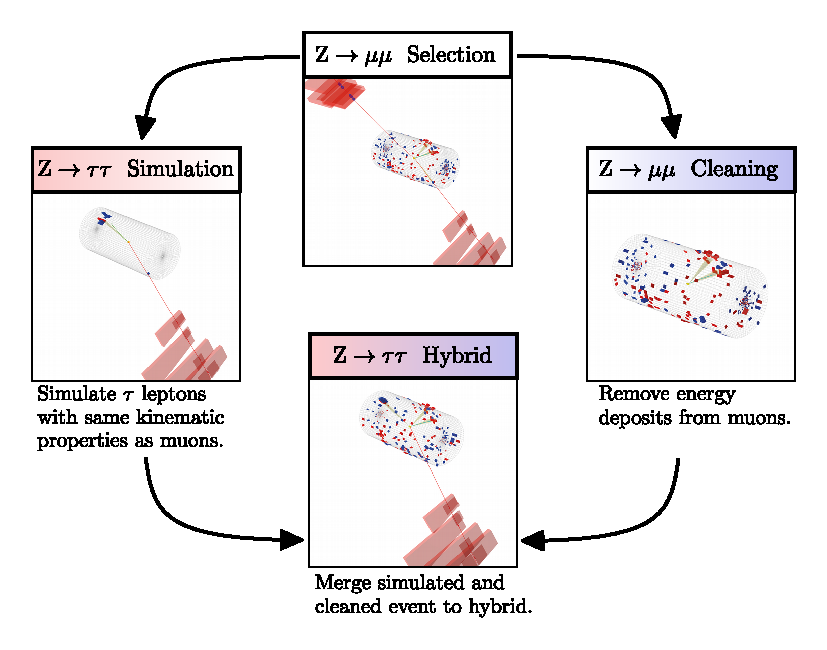
\includegraphics[width=0.8\textwidth]{Figures/Embedding_Diagram.pdf}
\caption{Schematic of the embedding method to model genuine di-tau backgrounds from di-muon events in data.}
\label{fig:embedding}
\end{figure}

The embedding method is validated on dedicated samples, where the muons from data are replaced by simulated muons instead of taus.

\newpage
\section{Fake Factor Method}
\label{sec:ff}

Backgrounds in which a jet fakes a $\tauh$ can be difficult to model using MC due to the poor description of the $\text{jet}\rightarrow\tauh$ fake rate in simulation. 
In addition, the small probability of a jet being misidentified as a $\tauh$ necessitates the production of high statistics MC samples at a significant computational expense.
These shortcomings motivate the use of data-driven estimates for these processes. 
One such procedure is the fake factor ($\FF$) method. \\

The $\FF$ method utilises regions in the data to model the $\text{jet}\rightarrow\tauh$ background. 
Firstly, the determination regions, which are $\text{jet}\rightarrow\tauh$ enriched control regions orthogonal to the signal region. 
It is used to calculate $\FF$ by taking the ratio of number of jet fake events that pass the nominal hadronic tau ID requirement ($N(\texttt{Nominal})$), to the number of jet fake events that fail the nominal hadronic tau ID but pass a looser alternative hadronic tau ID requirement ($N(\texttt{Alternative}~\&\&~\texttt{!Nominal})$), as shown in Equation~\ref{eqn:ff}.

\begin{equation}
\FF = \frac{N(\texttt{Nominal})}{N(\texttt{Alternative}~\&\&~\texttt{!Nominal})}.
\label{eqn:ff}
\end{equation}

In the remaining text this numerator and denominator are referred to as the pass and fail regions.
The derivation of this ratio is done differentially with respect to key parameters that differ in the two regions.
Once $\FF$ have been derived it is common to calculate corrections in other sideband regions (a region orthogonal to the signal region) and combine $\FF$ measured from different processes.
Finally, the $\FF$ are applied to the application region (AR). 
This is defined as the SR but with the criteria that the jet fakes fail the nominal hadronic tau ID but pass the looser alternative tau ID requirement.
This now models the background from $\text{jet}\rightarrow\tauh$ events in SR. \\

The following Sections~\ref{sec:ff_dr}--\ref{sec:ff_applying} detail the complexities of how this method is applied to this analysis.
For these searches the nominal hadronc tau ID used is the \texttt{Medium} $D_{\text{jet}^{\text{WP}}}$ and the alternative hadronic tau ID used is the \texttt{VVVLoose}  $D_{\text{jet}^{\text{WP}}}$.

\subsection{Determination Regions}
\label{sec:ff_dr}

The fake factors are measured separately in each year of data taking period (2016, 2017, 2018), in each channel containing hadronic taus ($\etauh$, $\mutauh$, $\tauhtauh$) and in enriched regions of dominant processes that contribute $\text{jet}\rightarrow\tauh$ events.
In the $\etauh$ and $\mutauh$ channels $\FF$ are measured for three processes: QCD, W + Jets and $\ttbar$.
In the $\tauhtauh$ channel $\FF$ are measured only for the dominant QCD process.
The QCD process is assumed to produce two jet fakes and so the fake factors is chosen to be calculated from leading $\pT$ hadronic tau candidate only. 
Section~\ref{sec:ff_applying} discusses how single jet fake events in the $\tauhtauh$ channel are modelled. \\

Each separate measurement region is split into three sideband regions based off two cuts that surround the signal region.
These regions are named the \texttt{Determination Region} (C), \texttt{Alternative Determination Region} (D) and \texttt{Correction Region} (B) and are schematically shown in Figure~\ref{fig:ff_schematic}. \\

\begin{figure}[!hbtp]
\centering
    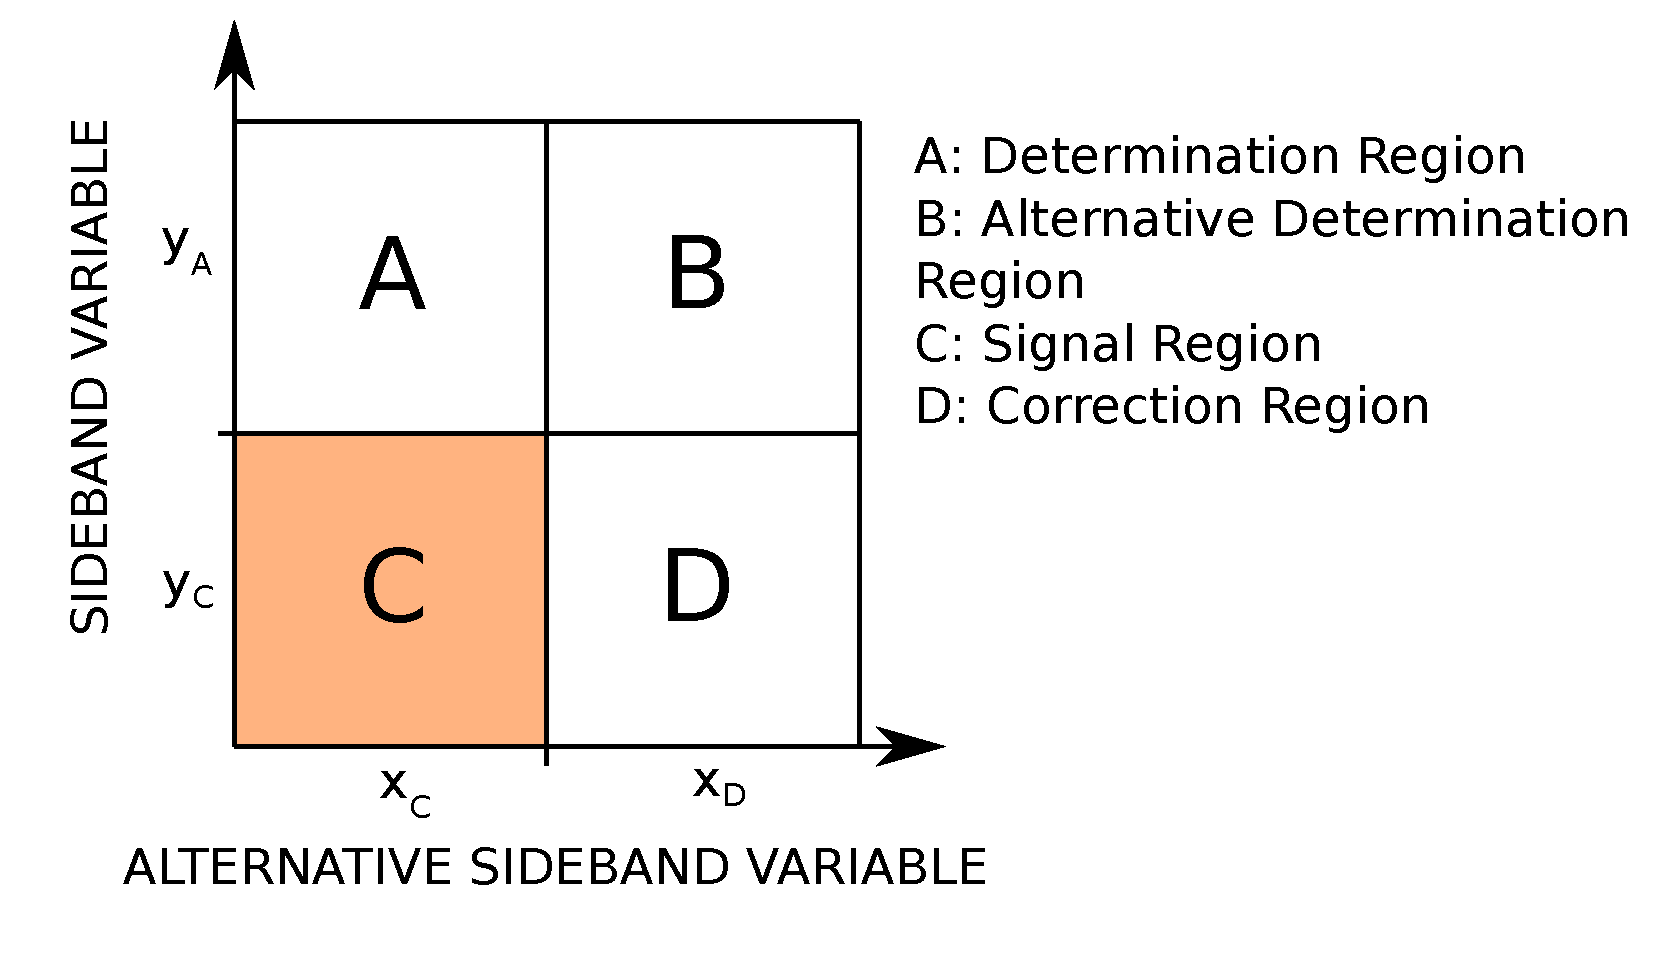
\includegraphics[width=0.8\textwidth]{Figures/ff_diagram_v2.pdf}
\caption{Schematic of the regions used for fake factor derivation.}
\label{fig:ff_schematic}
\end{figure}

Region A is used to measure and fit fake factors.
Region B is an alternative region used to measure and fit fake factor to account for the difference in fake factors between A and C.
These alternative fake factors are applied to the fail region in D and corrections are calculated comparing it to the pass region in D.
The total fake factor per measurement region is calculated as the fake factors derived in region A multiplied by the correction calculated from region B to D. \\

The selection for $x_C$, $x_D$, $y_C$ and $y_A$, as defined in Figure~\ref{fig:ff_schematic}, in each separate measurement region are shown below.
These are chosen to balance the number of events and the purity of each background in the region.

\begin{enumerate}[i)]
   \item $\tauhtauh$ QCD \\
     \indent $y_C$: The $\tauh$ candidates are required to have the opposite sign. \\
     \indent $y_A$: The $\tauh$ candidates are required to have the same sign. \\
     \indent $x_C$: The subleading tau passes the \texttt{Medium} $D_{\text{jet}}^{\text{WP}}$. \\
     \indent $x_D$: The subleading tau fails the \texttt{VVLoose} $D_{\text{jet}}^{\text{WP}}$ but passes the \texttt{VVVLoose} $D_{\text{jet}}^{\text{WP}}$.
  \item $\etauh$ and $\mutauh$ QCD \\
    \indent $y_C$: The $e$/$\mu$ and $\tauh$ candidates are required to have the opposite sign. \\
    \indent $y_A$: The $e$/$\mu$ and $\tauh$ candidates are required to have the same sign and the $e$/$\mu$ to have $\Irel>0.05$. \\
    \indent $x_C$: The $e$/$\mu$ candidate is required to have $\Irel<0.15$. \\
    \indent $x_D$: The $e$/$\mu$ candidate is required to have $0.25<\Irel<0.5$.
  \item $\etauh$ and $\mutauh$ W + Jets \\
    \indent $y_C$: The $\mT$ between the $e$/$\mu$ and the MET $< 70$ GeV. \\
    \indent $y_A$: The $\mT$ between the $e$/$\mu$ and the MET $> 70$ GeV and no b jets in the event. \\
    \indent $x_C$: Data. \\
    \indent $x_D$: W + Jets MC.
  \item $\etauh$ and $\mutauh$ $\ttbar$ \\
    \indent $y_C$: Data. \\
    \indent $y_A$: MC ($\ttbar$ in B and W + Jets D). \\
    \indent $x_C$: $\mT < 70$ GeV. \\
    \indent $x_D$: $\mT > 70$ GeV and no b jets. \\
\end{enumerate}


In the $\mu\tauh$ and $e\tauh$ channels QCD and W + Jets jet fake events are in general the most significant and contribute with approximately equal weights. 
$\ttbar$ inclusively is small but becomes more significant when searching for events with a b jet. 
The additional $\Irel>0.05$ requirement in these channels for QCD is to reduce processes producing genuine leptons and the $N_{\text{b-jets}}=0$ requirement for W + Jets is to reduce $\ttbar$ contamination.
It is not possible to define a DR that is sufficiently pure in $\ttbar$ events to make a reasonable measurement of $\FF^{\ttbar}$ from data.
Therefore $\FF^{\ttbar}$ are derived from MC. 
A comparison of the $\FF^{\text{W+jets}}$ measured in data and MC shows only $\sim$ 10--20\% differences in the fake rates in data and MC.  
This observation coupled with the fact that the $\ttbar$ contribution is small compared to the other processes means that any bias introduced by using $\FF^{\ttbar}$ measured in MC is small compared to the uncertainties on the fake factors, discussed in Section~\ref{sec:uncertainties}. \\


\subsection{Parametrisation}

The raw $\FFi$ take into account dependencies on $N_{\text{jets}}$ via the analysis tailed variable $N_{\text{pre b-jets}}$, the $\pT$ of the $\tauh$ candidate ($\pT^{\tauh}$) and the $\pT$ of the jet matched in $\Delta R$ to the $\tauh$ ($\pT^{\text{jet}}$).
$N_{\text{pre b-jets}}$ is defined to map the dependence of $\FFi$ on $N_{\text{jets}}$ and describe the categorising variable $N_{\text{b-jets}}$ well.
Although not local to the tau, it helps control other dependencies on the constituents of the event.
It is the number of jets in the event with $|\eta|<2.4$ and $\pT>20$. These are the same $\eta$ and $\pT$ thresholds required for a b-jet.
The data is split into two bins of $N_{\text{pre b-jets}}$, equal to 0 and greater than 0.
It is then further split by the ratio of $\pT^{\text{jet}}$ to $\pT^{\tauh}$.
An example of the dependence of these two transverse momentums on the fake factor is shown in Figure~\ref{fig:ff_colz}.

\begin{figure}[!hbtp]
\centering
    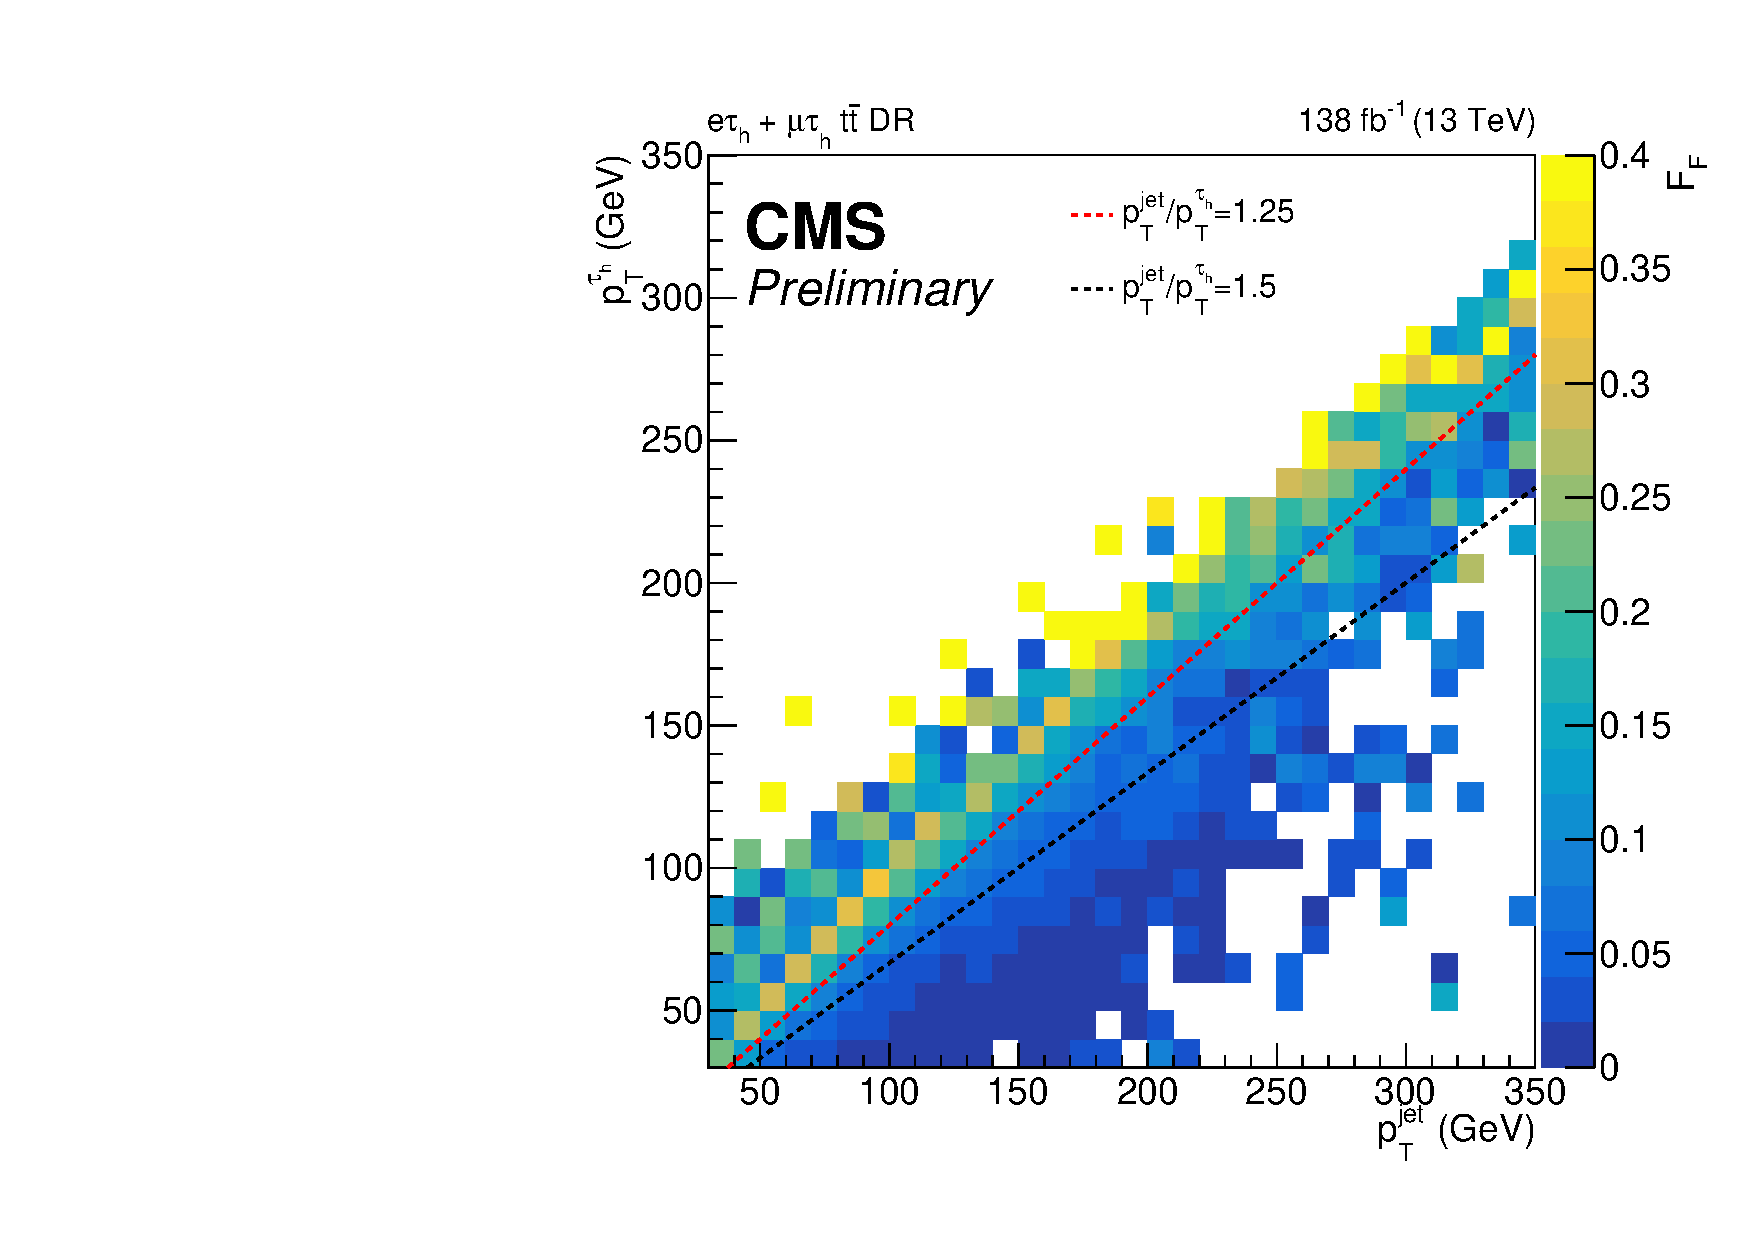
\includegraphics[width=0.6\textwidth]{Figures/ff_colz_ttbar_lt.pdf}
\caption{A 2D heat map of the fake factors determined from $t\bar{t}$ MC for the full run-2 dataset in the combined $e\tauh$ and $\mu\tauh$ channels. This is shown with respect to the hadronic tau $\pT$ and the $\pT$ of the jet matched to the hadronic tau. The ratio of jet to hadronic tau $\pT$ categorisation used is shown split by the dashed lines.}
\label{fig:ff_colz}
\end{figure}

It is motivated by the observation that the fake factor is largest when the $\pT^{\text{jet}}$ and $\pT^{\tauh}$ are closest.
The physical motivation for this is when they are close, the hadronic tau candidate is likely to be isolated from any other hadronic activity and so more likely to be identified as a tau.
However, when $\pT^{\text{jet}}$ is larger than $\pT^{\tauh}$, the candidate is likely surrounded by other hadronic activity and so more likely to be a jet fake.
When $\pT^{\text{jet}}$ is less than $\pT^{\tauh}$, charge pions are likely not close enough to the PV to be clustered into the jet and so the event is more likely to be classified as a jet fake. 
This will then lead to the fake factor dependence as seen in Figure~\ref{fig:ff_colz}.\\

For all divisions of the phase space, dependence on the $\pT^{\tauh}$ is fit using the superposition of a Landau and a zeroth order polynomial in the low-$\pT$ region.
The fake factors are seen to rise sharply at high-$\pT$.
This increase happens in either the bin 140 $<$ $\pT^{\tauh}$ $<$ 200 GeV or $\pT^{\tauh}$ $>$ 200 GeV.
To map this effect, binned values are taken based off the algorithm shown in Figure~\ref{fig:ff_binning} and the fit is used below the minimum bin.

\begin{figure}[!hbtp]
  \centering
  \begin{tikzpicture}[node distance = 8cm, auto]
    % nodes
    \node [block] (start) {Fractional Error in $\pT$ (GeV) Bin, $\frac{\Delta N}{N}$.};
    \node [decision, aspect=2, node distance=5cm, right of = start] (d1) {[140,200)};
    \node [decision, aspect=2, node distance=3cm, above of = d1] (d2) {[200,$\infty$)};
    \node [decision, aspect=2, node distance=3cm, below of = d1] (d3) {[200,$\infty$)};
    \node [block3, aspect=2, node distance=3cm, above of = d2] (n1) {Use bin values in [140,200,$\infty$)};
    \node [block3, aspect=2, node distance=3cm, below of = d3] (n2) {Use bin values in [200,$\infty$)};
    \node [block3, aspect=2, node distance=5cm, right of = d2] (n3) {Use bin values in [140,$\infty$)};
    \node [block3, aspect=2, node distance=5cm, right of = d3] (n4) {Use no bins};
    % edges
    \draw [arrow] (start) -- (d1);
    \draw [arrow] (d1) -- node[anchor=east] {$>0.5$} (d2);
    \draw [arrow] (d1) -- node[anchor=east] {$<0.5$} (d3);
    \draw [arrow] (d2) -- node[anchor=east] {$>0.5$} (n1);
    \draw [arrow] (d2) -- node[anchor=south] {$<0.5$} (n3);
    \draw [arrow] (d3) -- node[anchor=east] {$>0.5$} (n2);
    \draw [arrow] (d3) -- node[anchor=south] {$<0.5$} (n4);
  \end{tikzpicture}
  \vspace{1cm}
  \caption{Flow chart of the algorithm used to determine where binned values are taken instead of the fit. The blue box represents the input, the green diamonds represent the decisions and the red boxes represent the outputs.}
  \label{fig:ff_binning}
\end{figure}

The Landau and zeroth order polynomial fits are flattened at $\pT^{\tau_h}$ values where there is no significant downwards shift or at the final bin. Fake factor fits with respect to $\pT^{\tau_h}$ are shown in Figures~\ref{fig:tt_ff_fit}-\ref{fig:mt_ff_fit}. The fake factors are highest in the lowest $\pT^{\text{jet}}/\pT^{\tau_h}$ bin and lowest in the highest bin as expected. Otherwise the fake factors fall with $\pT$ in each category until the thresholds used for the high $\pT$ binning algorithm.

\begin{figure}[!hbtp]
\centering
    \subfloat[]{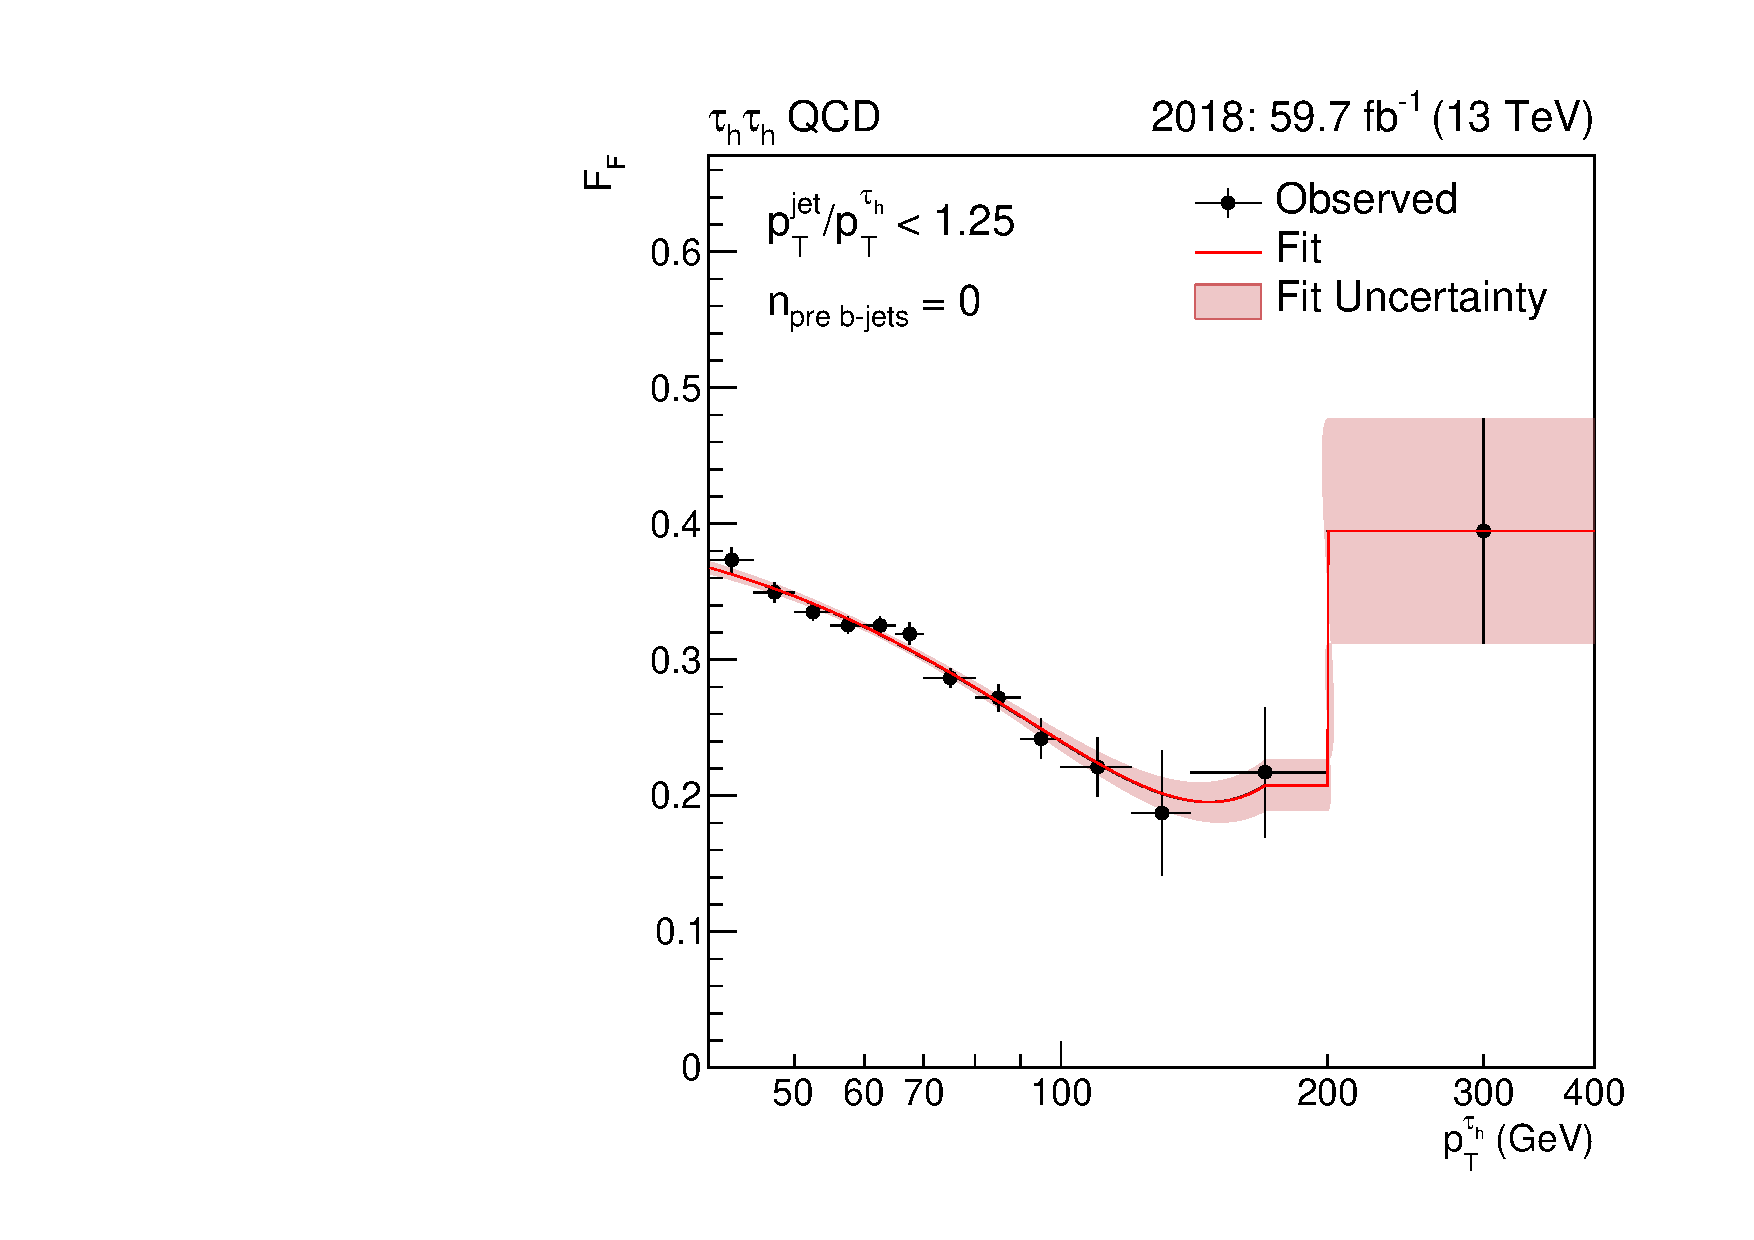
\includegraphics[width=0.33\textwidth]{Figures/ff_fit_jet_pt_low_0jet_pt_1_ff_qcd_tt_2018.pdf}}
    \subfloat[]{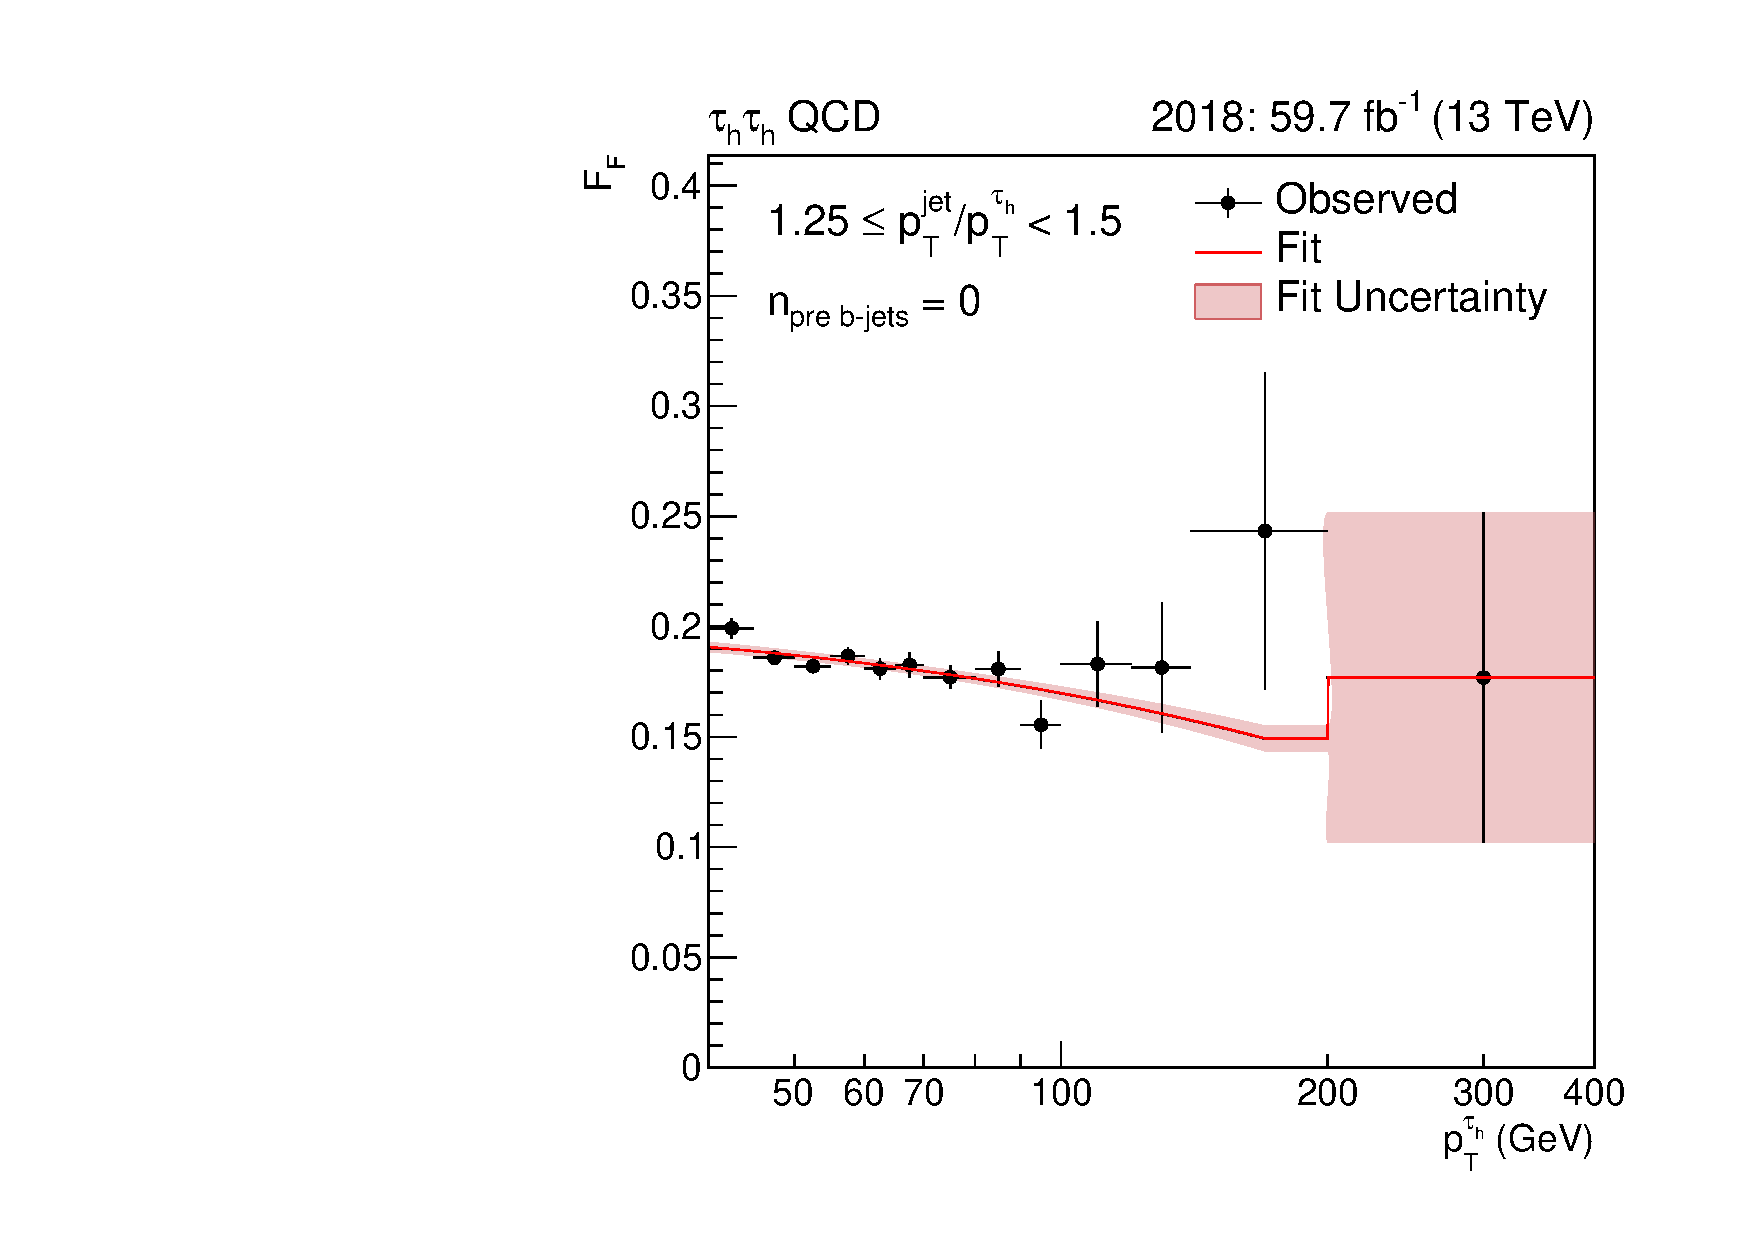
\includegraphics[width=0.33\textwidth]{Figures/ff_fit_jet_pt_med_0jet_pt_1_ff_qcd_tt_2018.pdf}} 
    \subfloat[]{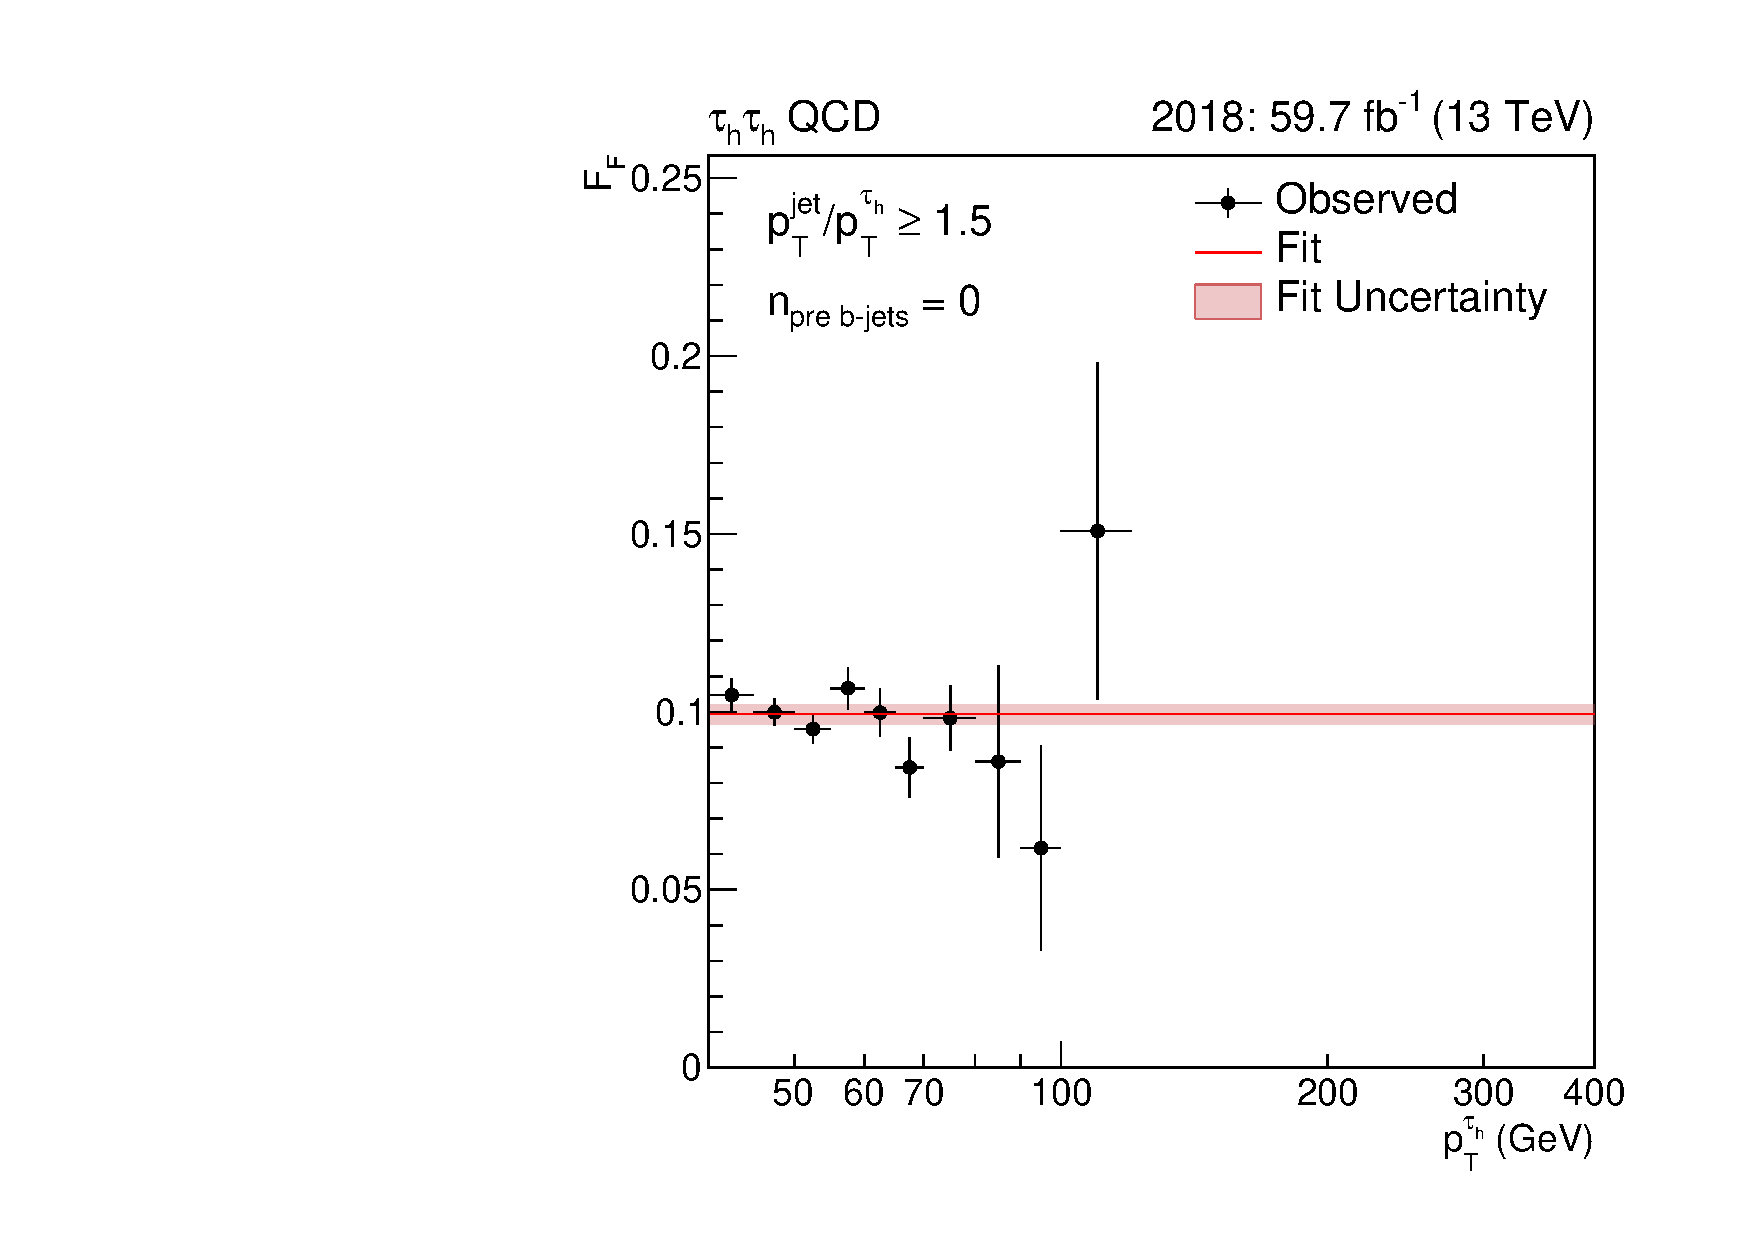
\includegraphics[width=0.33\textwidth]{Figures/ff_fit_jet_pt_high_0jet_pt_1_ff_qcd_tt_2018.pdf}} \\
\caption{Fake factor fits in $\tauh\tauh$ channel for the QCD $N_{\text{pre b jets}}=0$ category with 2018 data. The three jet $\pT$ to hadronic tau $\pT$ categories are shown.}
\label{fig:tt_ff_fit}
\end{figure}

\begin{figure}[!hbtp]
\centering
    \subfloat[]{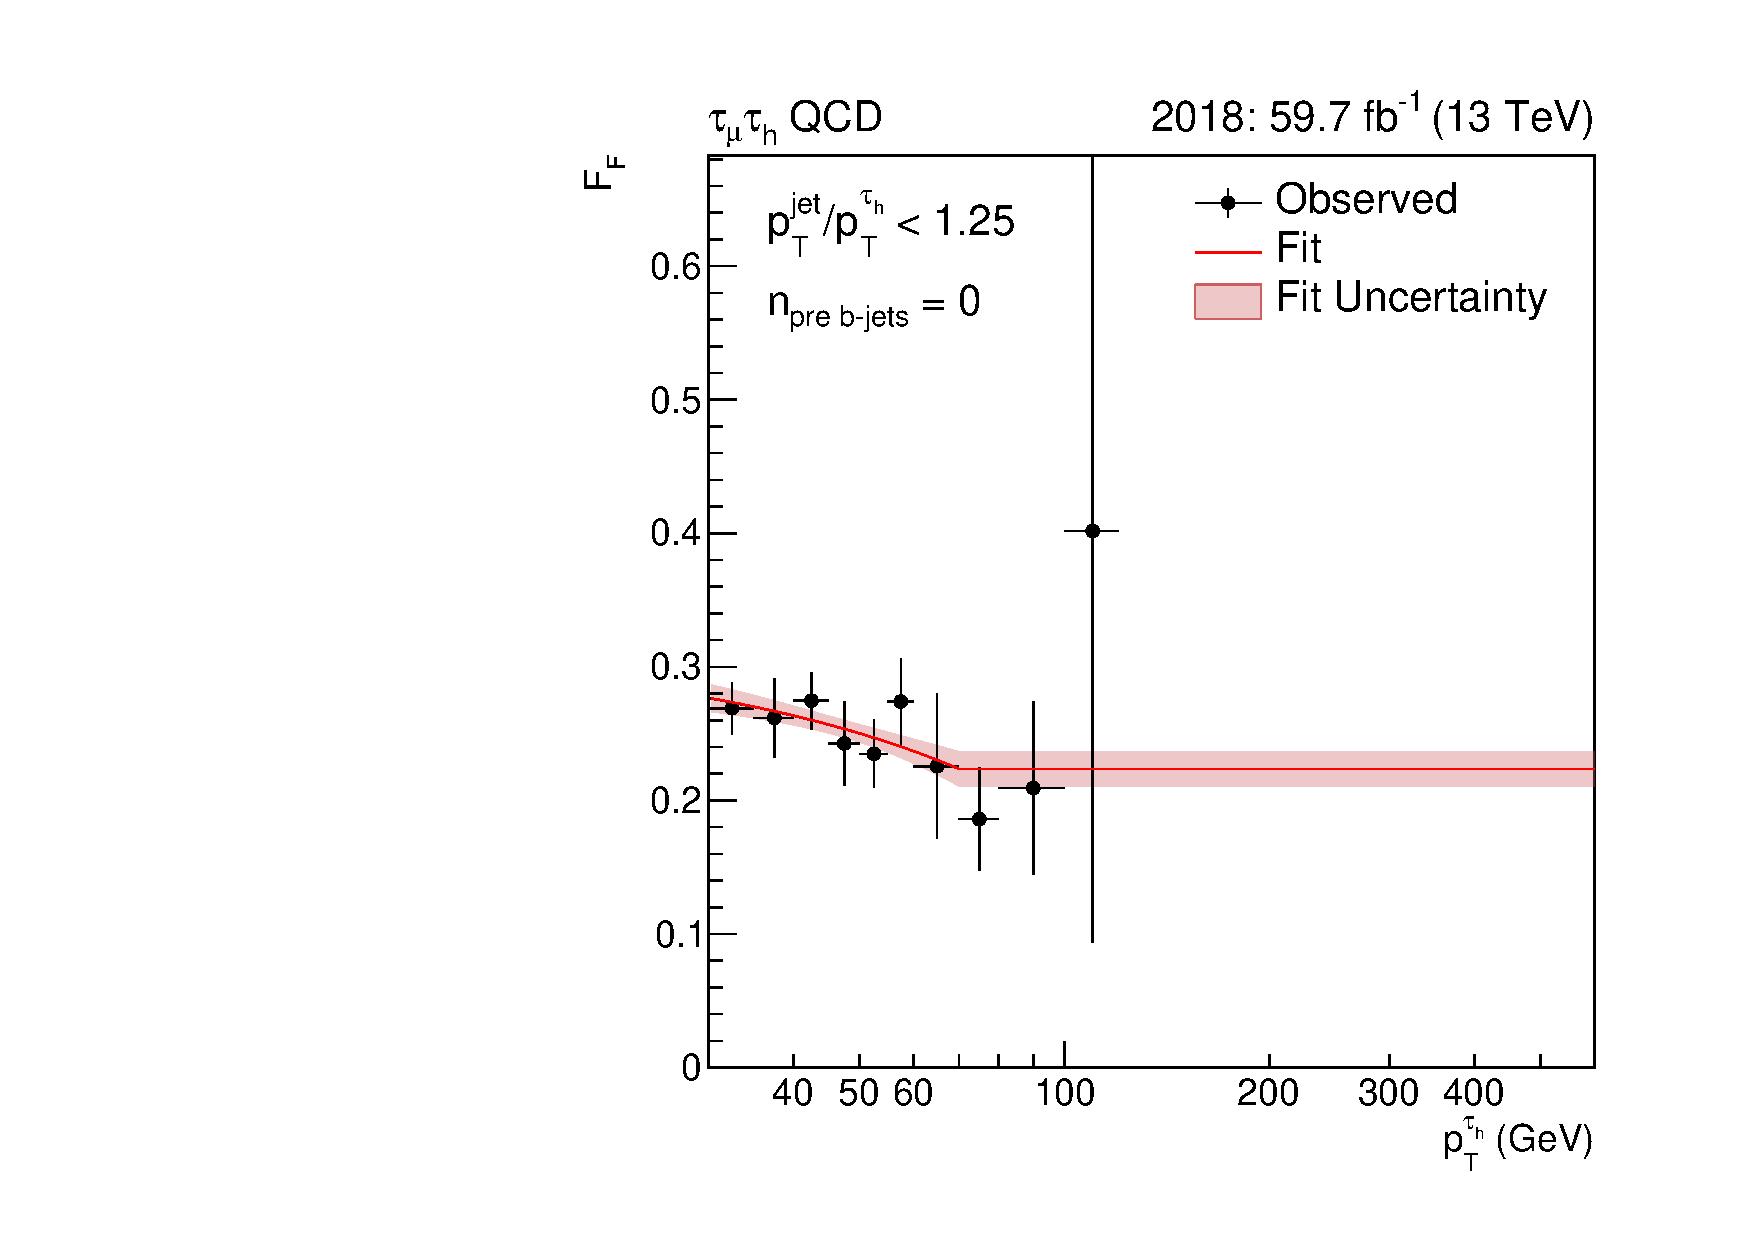
\includegraphics[width=0.33\textwidth]{Figures/ff_fit_jet_pt_low_0jet_pt_2_ff_qcd_mt_2018.pdf}}
    \subfloat[]{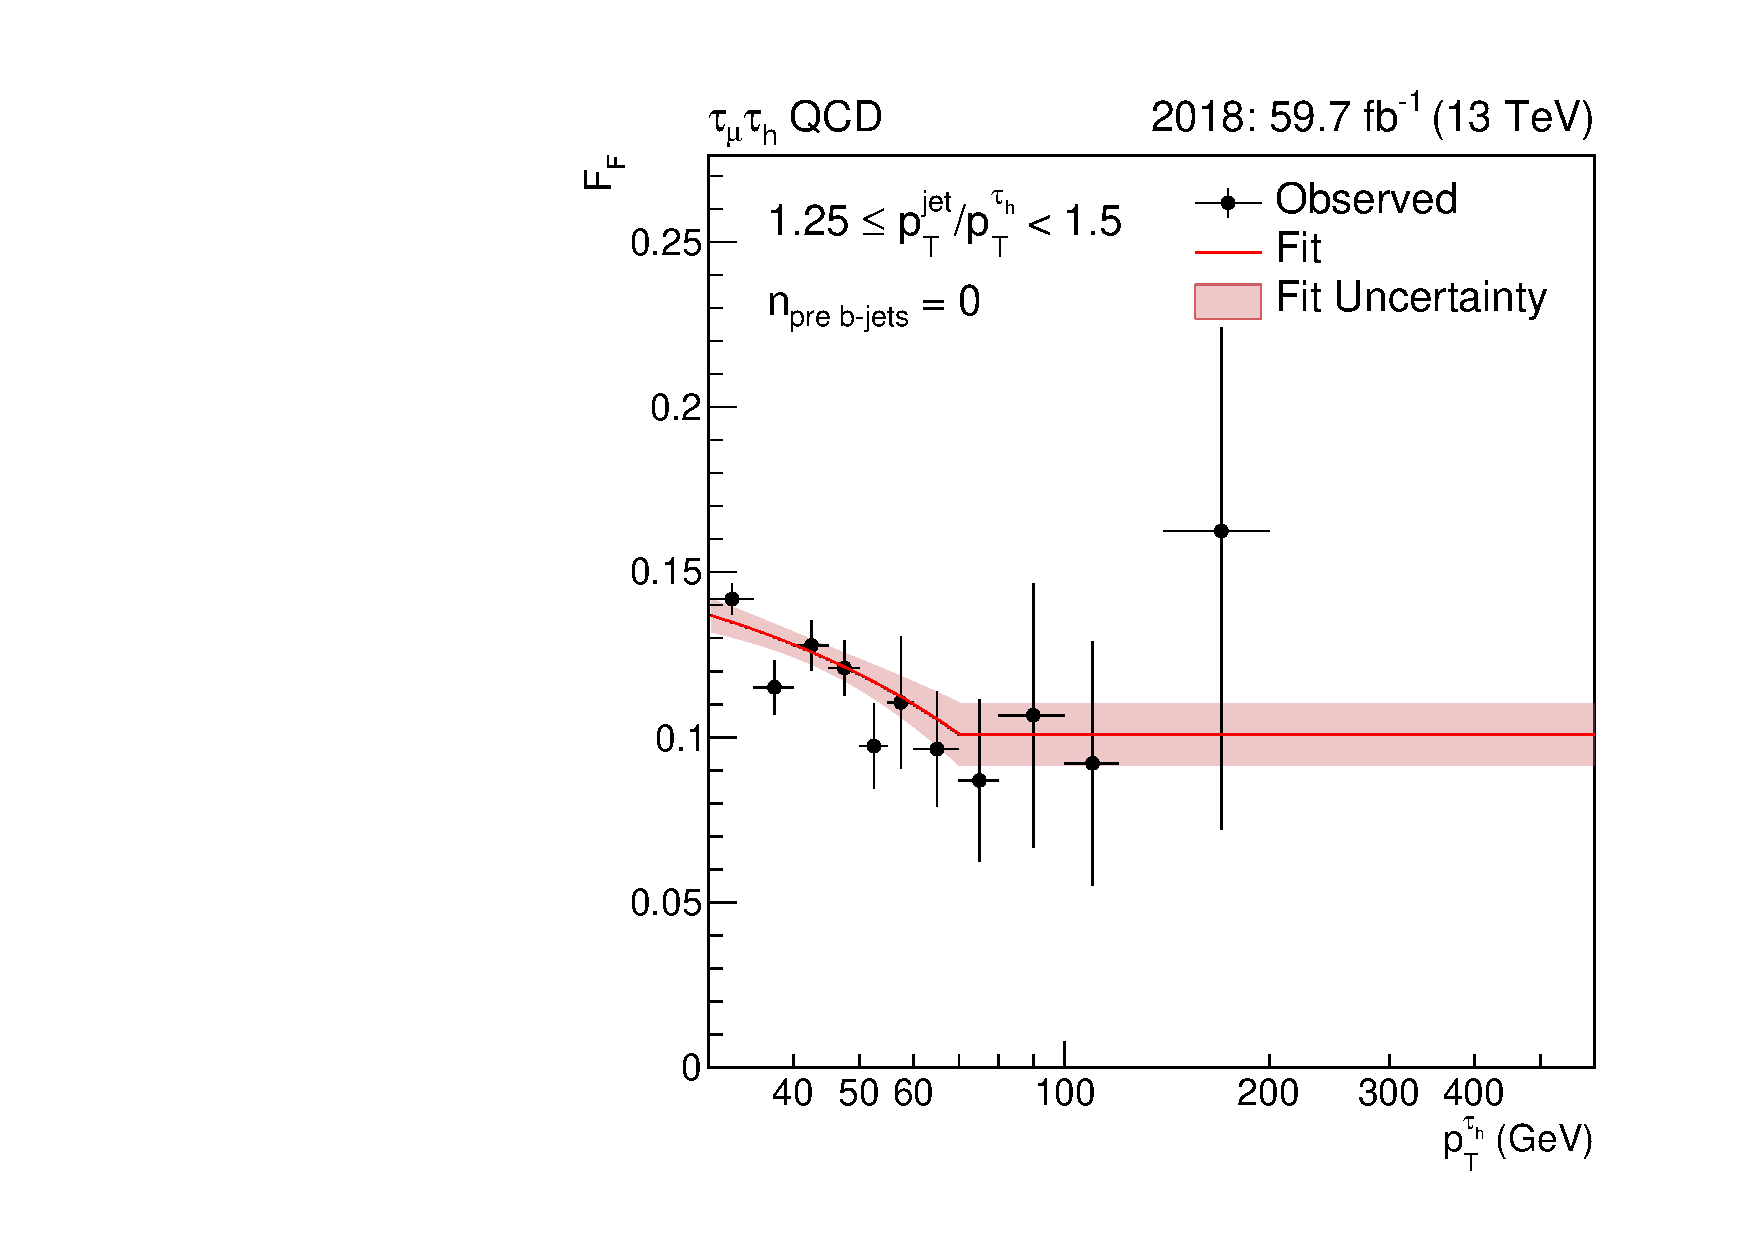
\includegraphics[width=0.33\textwidth]{Figures/ff_fit_jet_pt_med_0jet_pt_2_ff_qcd_mt_2018.pdf}} 
    \subfloat[]{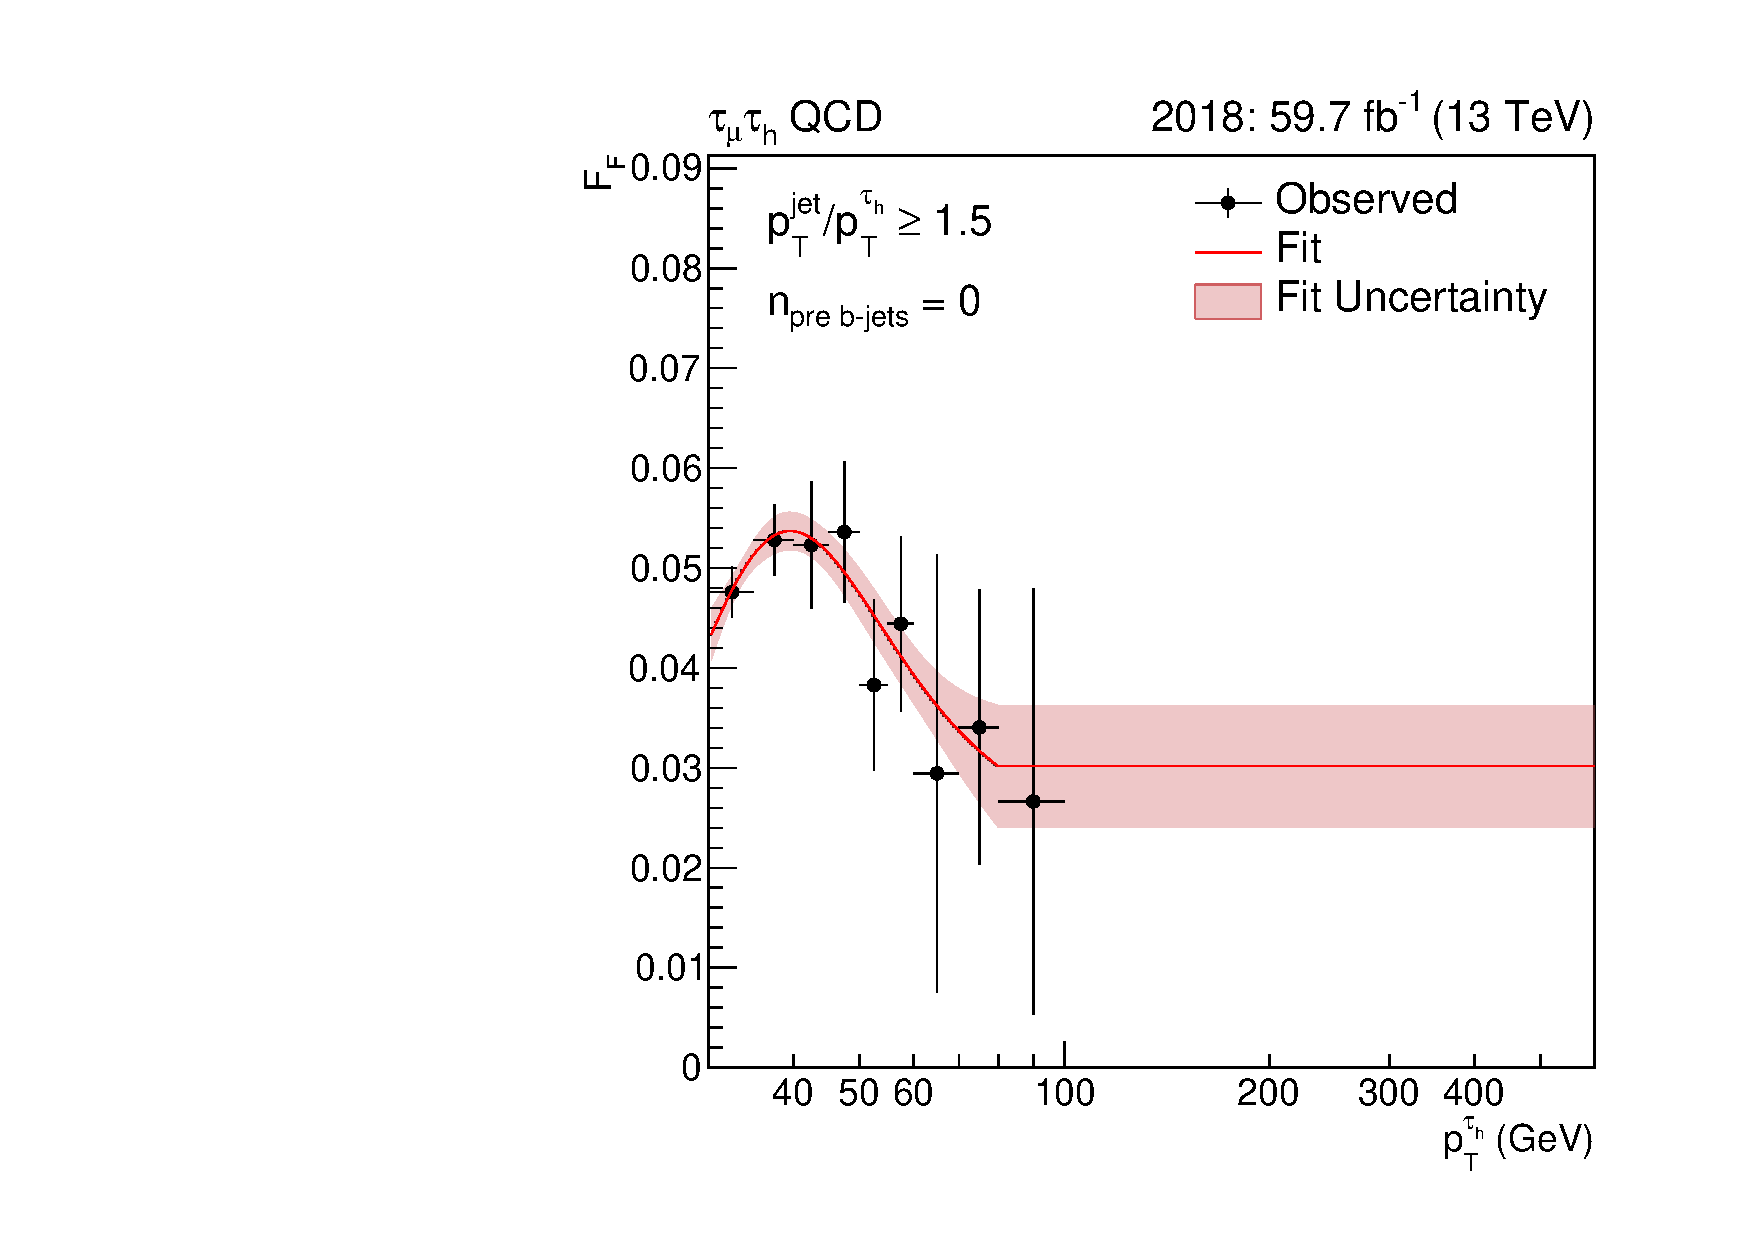
\includegraphics[width=0.33\textwidth]{Figures/ff_fit_jet_pt_high_0jet_pt_2_ff_qcd_mt_2018.pdf}} \\
    \subfloat[]{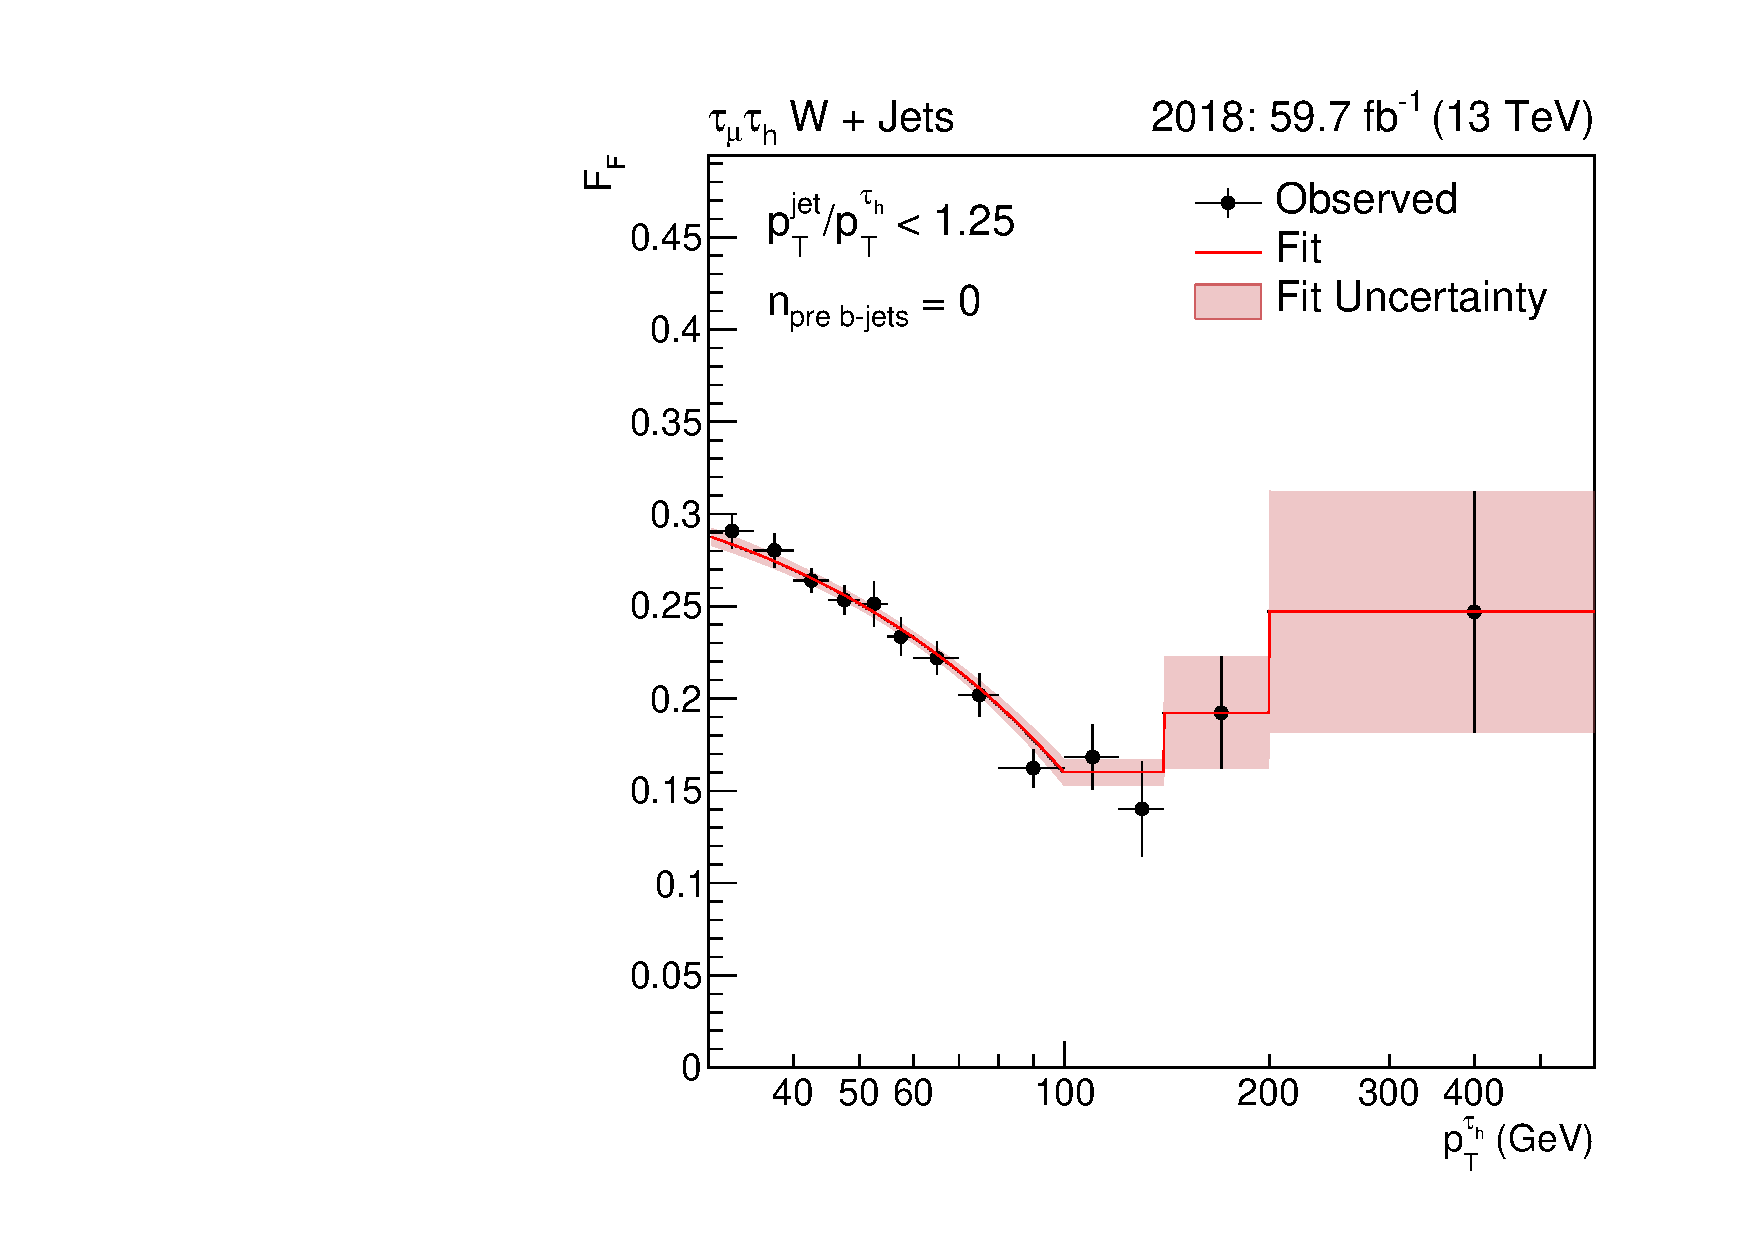
\includegraphics[width=0.33\textwidth]{Figures/ff_fit_jet_pt_low_0jet_pt_2_ff_wjets_mt_2018.pdf}}
    \subfloat[]{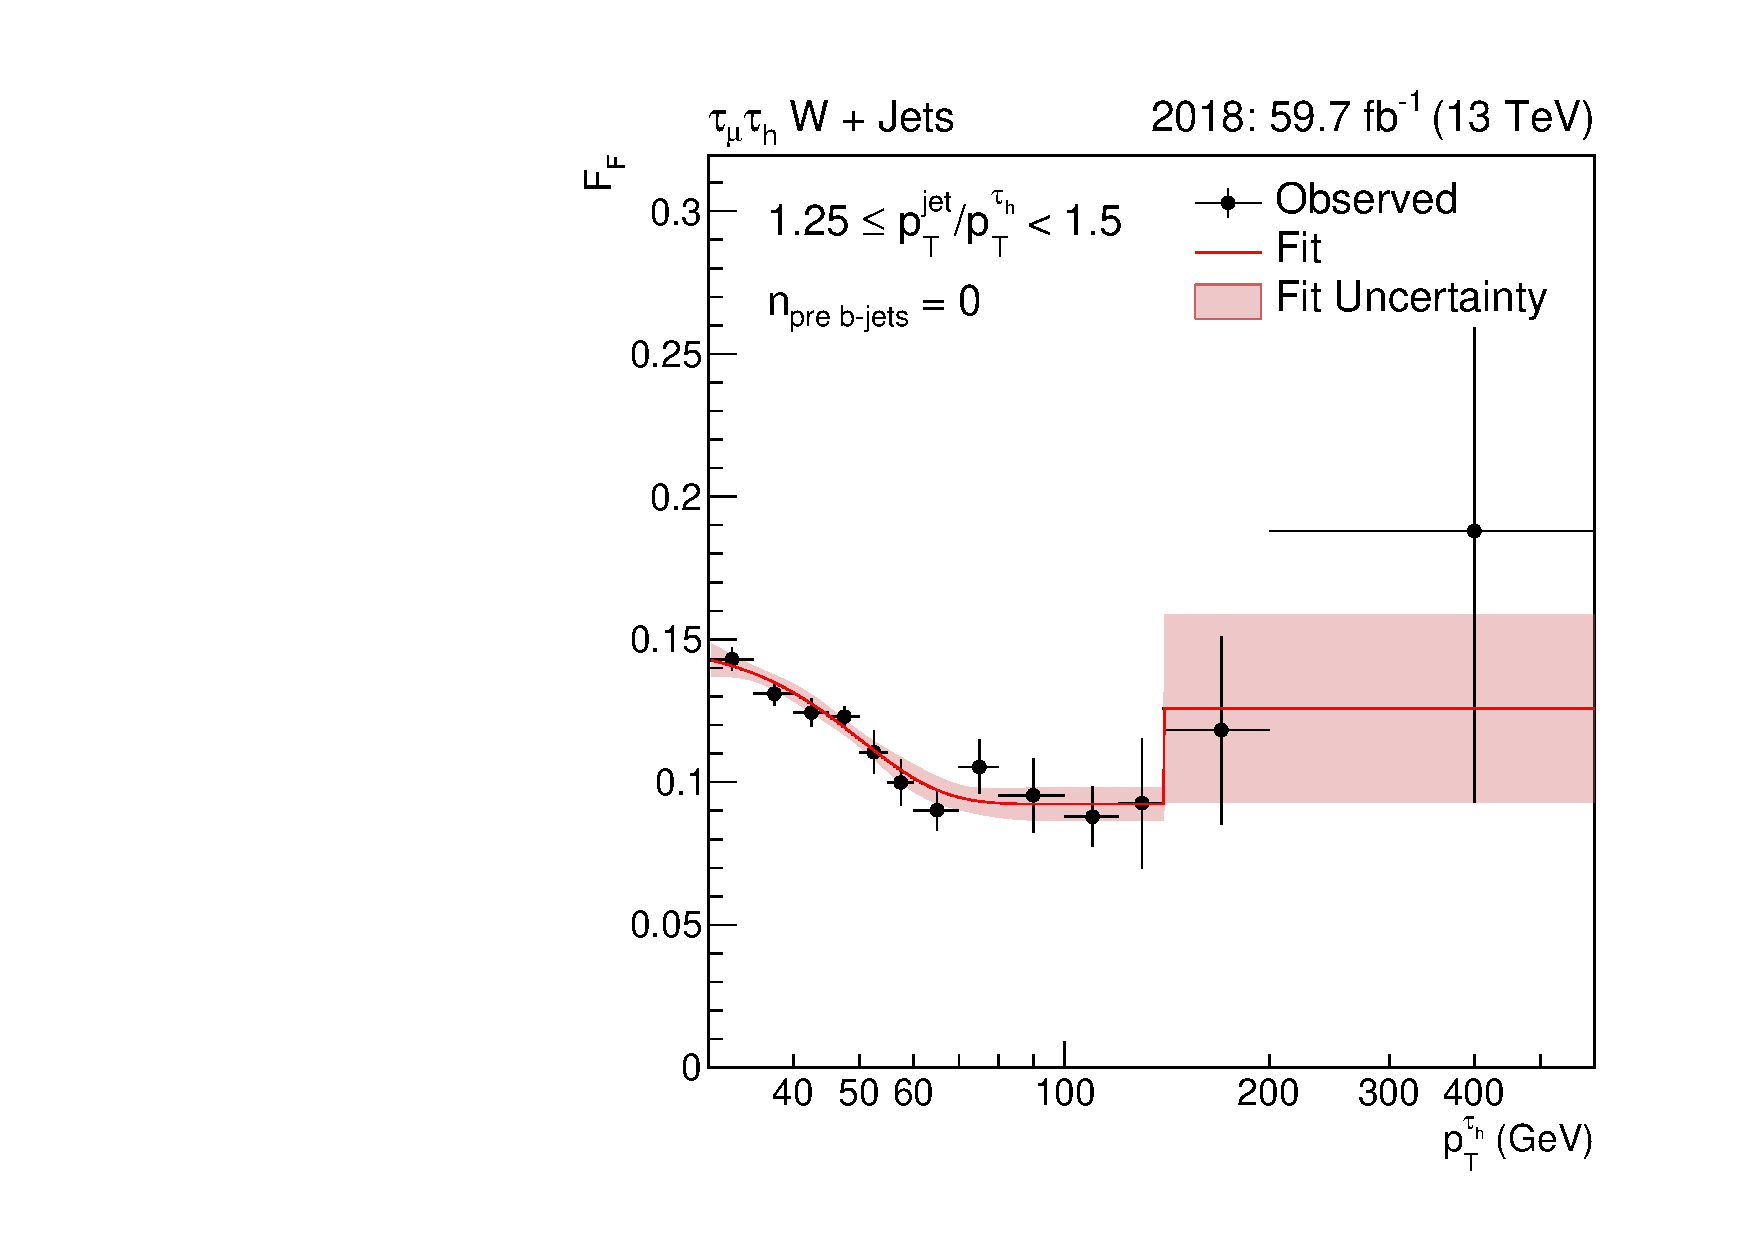
\includegraphics[width=0.33\textwidth]{Figures/ff_fit_jet_pt_med_0jet_pt_2_ff_wjets_mt_2018.pdf}} 
    \subfloat[]{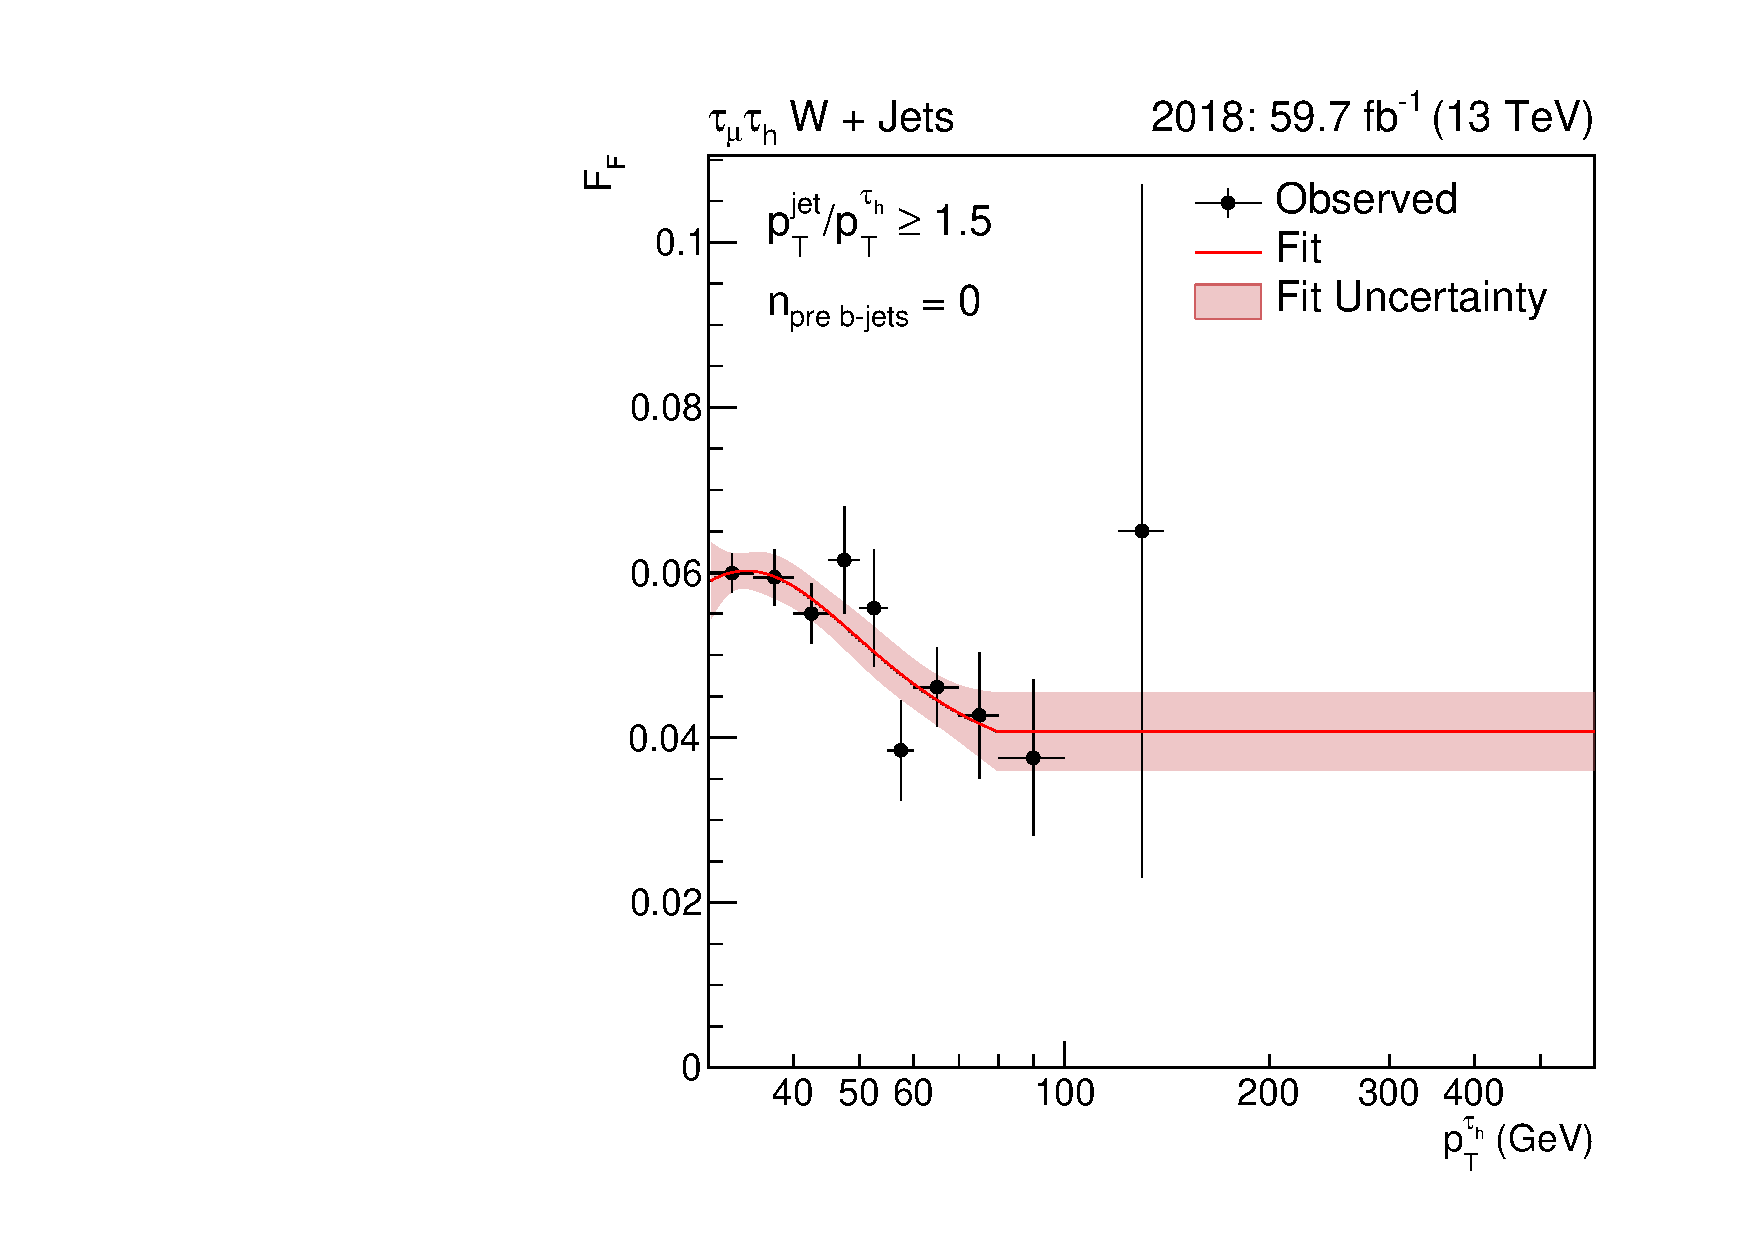
\includegraphics[width=0.33\textwidth]{Figures/ff_fit_jet_pt_high_0jet_pt_2_ff_wjets_mt_2018.pdf}} \\
\caption{Fake factor fits in $\mu\tauh$ channel for the QCD and W + Jets $N_{\text{pre b jets}}=0$ category with 2018 data. The three jet $\pT$ to hadronic tau $\pT$ categories are shown for each process.}
\label{fig:mt_ff_fit}
\end{figure}

\subsection{Corrections}

In the $\tauhtauh$ channel, the measured $\FF^{\text{QCD}}$ are then corrected to account for non-closures in other variable in the \texttt{Determination Region}. 
The only significance non-closures are observed for $\MET$ related variables and are largest for events with $N_{\text{pre b-jets}}=0$. 
Closure corrections are performed for the variable $\Delta R$ in bins of $N_{\text{b-jets}}$.
In the $\mutauh$ and $\etauh$ channels, the measured $\FF^{\text{QCD}}$ and $\FF^{\text{W+jets}}$ are corrected for non-closures observed in the $\MET$ variables and $\pT^{e/\mu}$ distributions.
A study was performed to determine the nature of these non-closures and it was found that the cause was due to fake $\MET$ arising from mismeasurement of the energies of particles in a jet. 
A diagram of this effect is shown in Figure~\ref{fig:fakemet}. \\

\begin{figure}[!hbtp]
\centering
   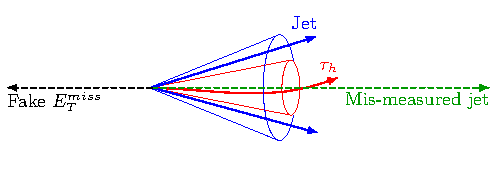
\includegraphics[width=\textwidth]{Figures/fakemet_plot.pdf}
\caption{Diagram showing how fake $\MET$ arises from mismodelling jet constituents in hadronic tau identification.}
\label{fig:fakemet}
\end{figure}

To correct for this effect, the QCD fake factors are corrected as a function of $C_{\text{QCD}}$, where $C_{\text{QCD}}$ is defined as,
\begin{equation}
C_{\text{QCD}} = \frac{\MET \cos\Delta\phi(\pTvec^{\text{\hspace{2pt}miss}},\pTvec^{\hspace{2pt}\tauh})}{\pT^{\tauh}}.
\label{eqn:c_qcd}
\end{equation}
where $\Delta\phi(\pTvec^{\hspace{2pt}\text{miss}},\pTvec^{\hspace{2pt}\tauh})$ is the separation in the azimuthal angle between the the missing a $\pTvec^{\text{miss}}$ and $\pTvec^{\tauh}$.
The numerator quantifies the missing transverse momentum in the direction of the hadronic tau candidate. 
Once divided by the $\tauh$ $\pT$, $C_{\text{QCD}}$ is a measure of the fraction of missing to visible hadronic tau transverse momentum aligned with the hadronic tau.
For W + jets and $\ttbar$ the situation is slightly different due to the presence of genuine missing energy from neutrinos.
In this case, the correction variable is modified to approximately subtract the genuine $\MET$ from the total.
This approximation assumes the neutrino is back-to-back and balanced with the light lepton (which is exactly true for W bosons produce at rest in the transverse direction). 
The equation then becomes,
\begin{equation}
C_{\text{W}} = \frac{(\MET+\pT^{e/\mu}) \cos\Delta\phi(\pTvec^{\text{\hspace{2pt}miss}}+\pTvec^{\hspace{2pt}e/\mu},\pTvec^{\hspace{2pt}\tauh})}{\pT^{\tauh}}.
\label{eqn:c_w}
\end{equation}
When either correction variable is separated from 0, a larger quantity of fake $E_{T}^{\text{miss}}$ is expected in the event. 
In these regions a large correction is needed due to the mis-measured jet energy spectrum shifting the hadronic tau candidate isolation and so shifting the tau identification scores. 
Examples of these closure corrections are shown in Figure~\ref{fig:ff_dr}\\

\begin{figure}[!hbtp]
\centering
    \subfloat[]{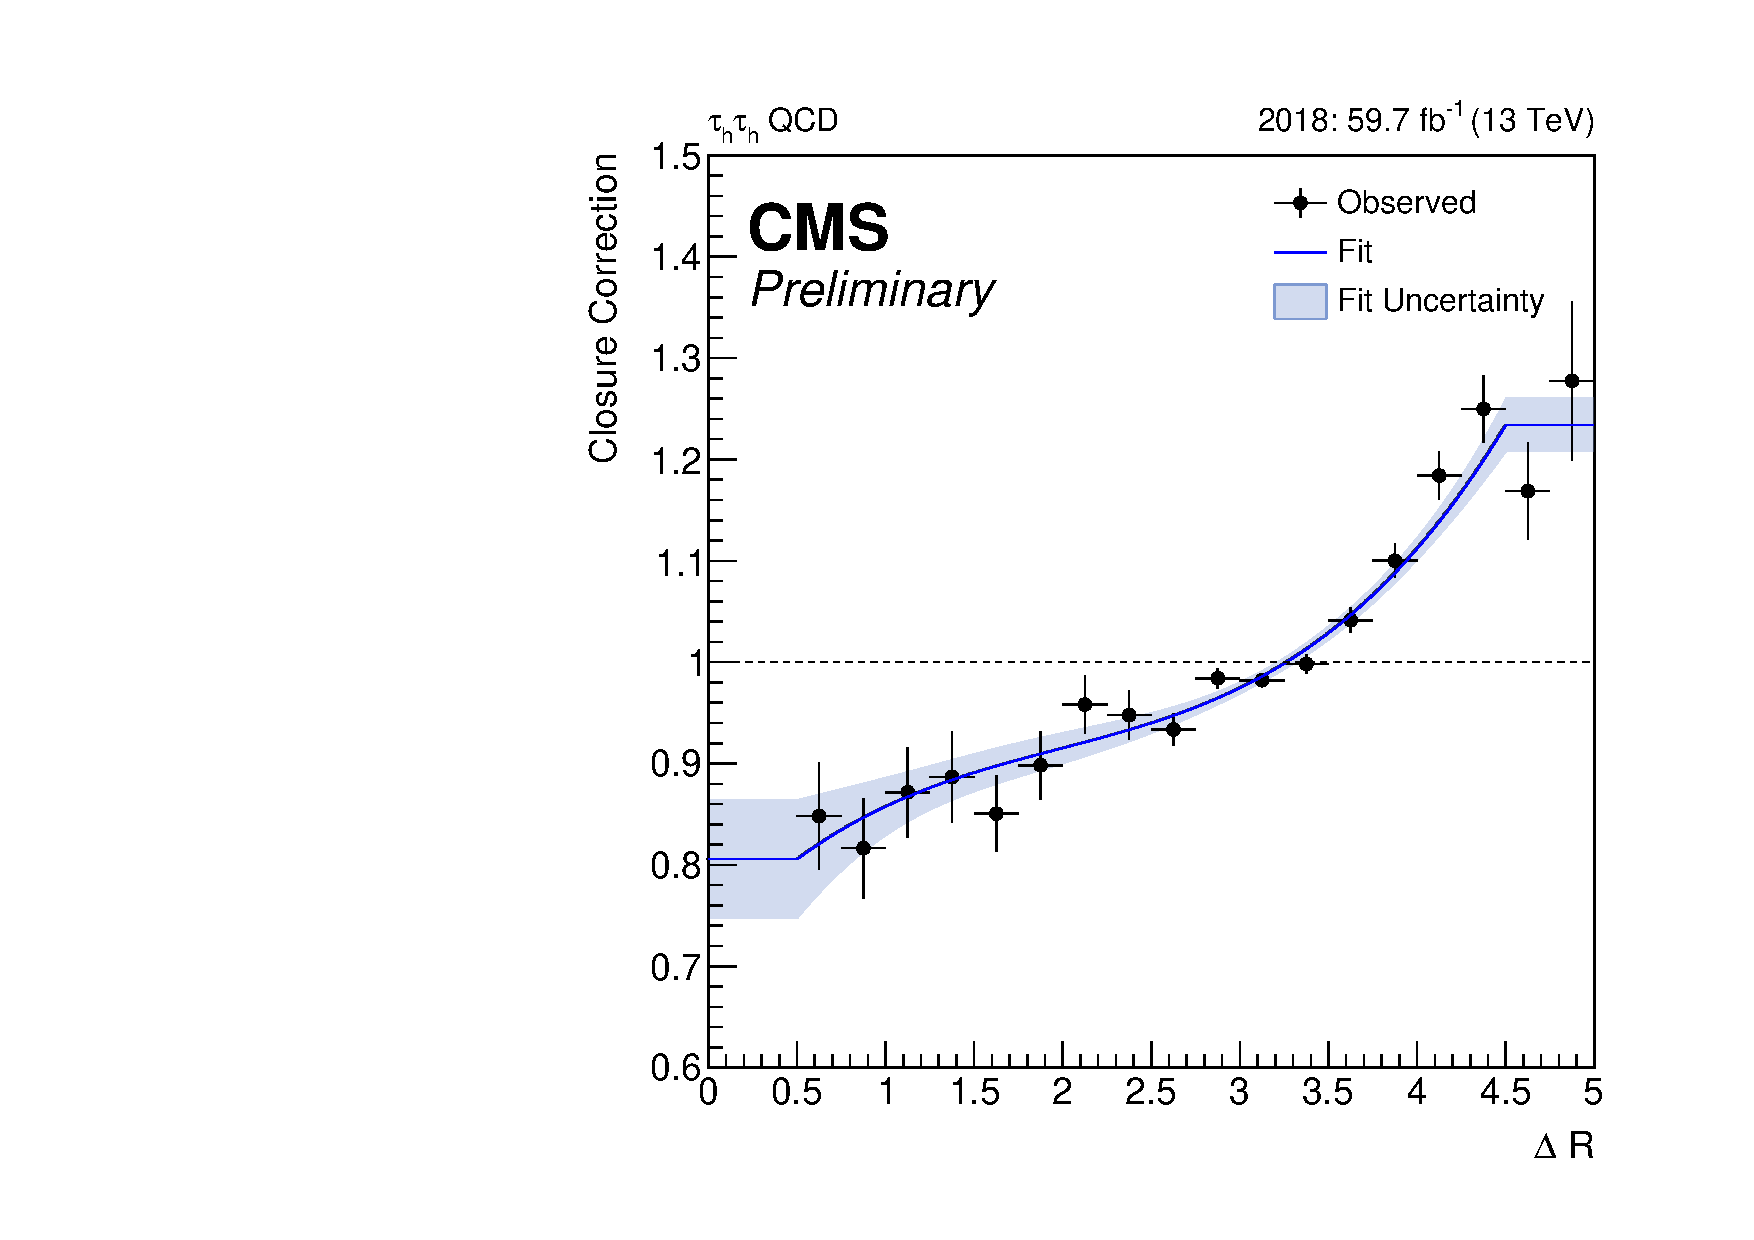
\includegraphics[width=0.33\textwidth]{Figures/ff_closure_ss_closure_nbjet0_qcd_tt_2018.pdf}} 
    \subfloat[]{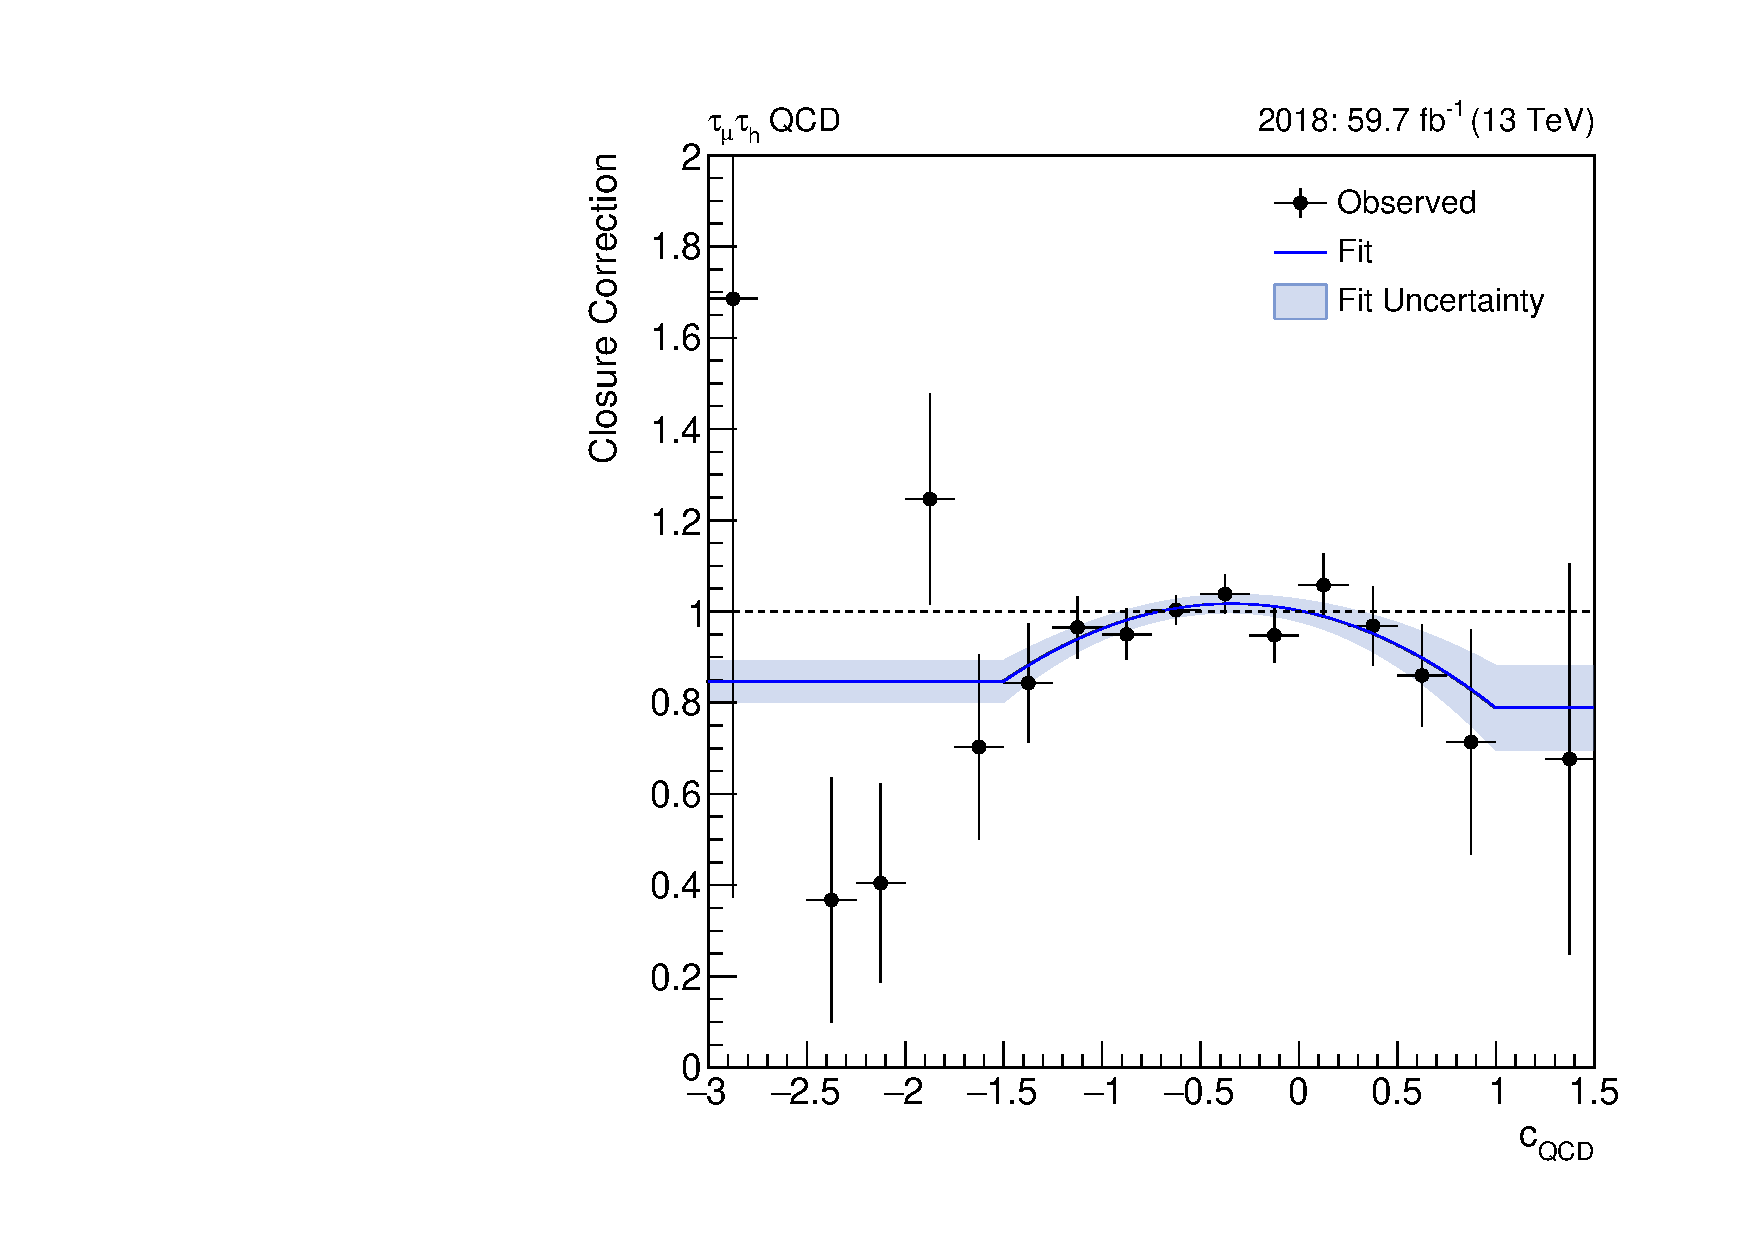
\includegraphics[width=0.33\textwidth]{Figures/ff_closure_met_0jet_closure_qcd_mt_2018.pdf}}
    \subfloat[]{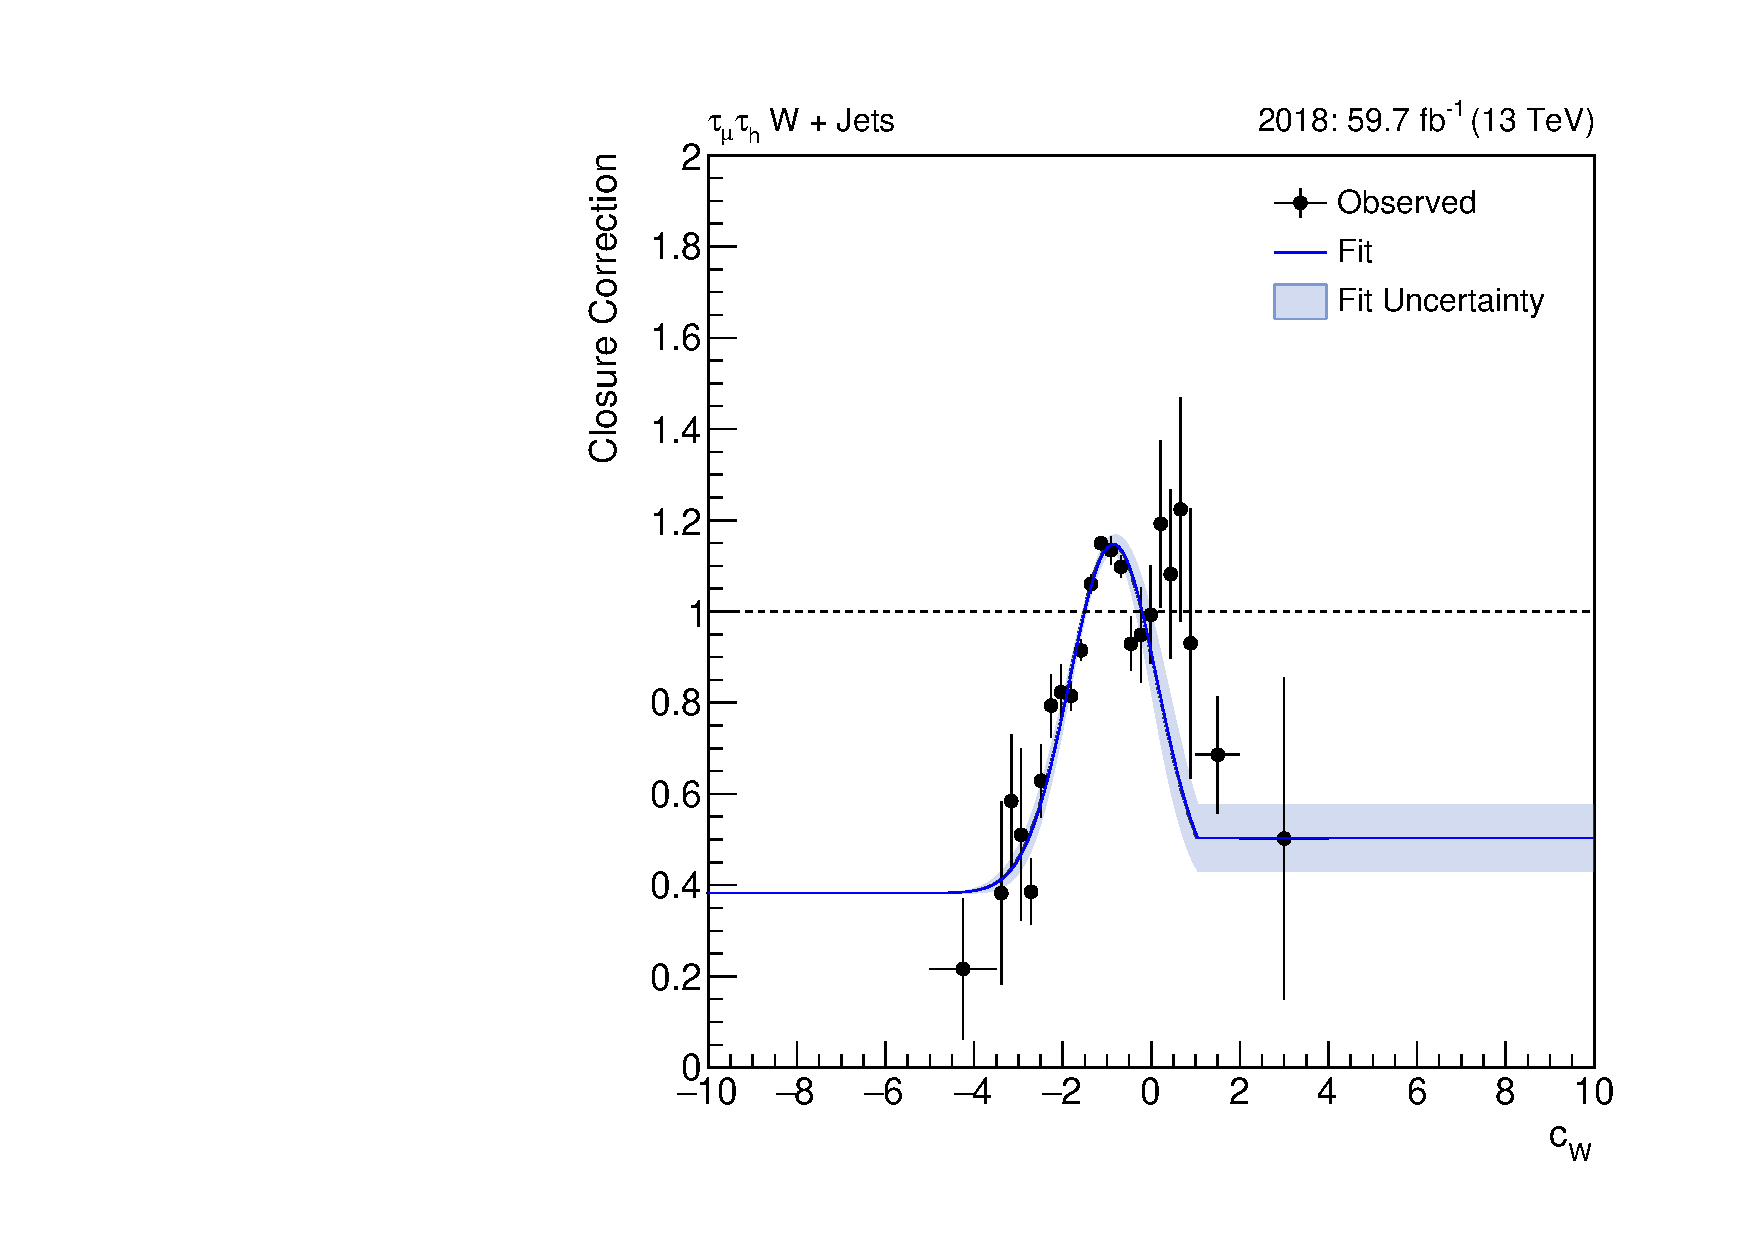
\includegraphics[width=0.33\textwidth]{Figures/ff_closure_met_0jet_closure_wjets_mt_2018.pdf}}
\caption{Determination region closure correction fits with 2018 data. (a) is the correction parametrised by $\Delta R$ in events with $N_{\text{b jets}}=0$ in the $\tauhtauh$ channel. (b) and (c) show the correction for the $\mutauh$ channel parametrised by the specific correction variables defined in Equation~\ref{eqn:c_qcd} and \ref{eqn:c_w} for QCD and W + jets processes respectively.}
\label{fig:ff_dr}
\end{figure}

After the \texttt{Determination Region} is modelled well for all variables of interest, extrapolation corrections from the fake factors derived in B applied to region D are calculated.
In the $\tauhtauh$ the correction is parameterised by the $p_{T}$ of the leading hadronic tau candidate, in the $\etauh$ and $\mutauh$ channels it is parameterised by the $\pT$ of the light lepton.
Where statistics allow, these corrections are calculated in the high mass optimisation procedure categories.
Examples of the extrapolation corrections are shown in Figure~\ref{fig:ff_dr_to_ar}.


\begin{figure}[!hbtp]
\centering
    \subfloat[]{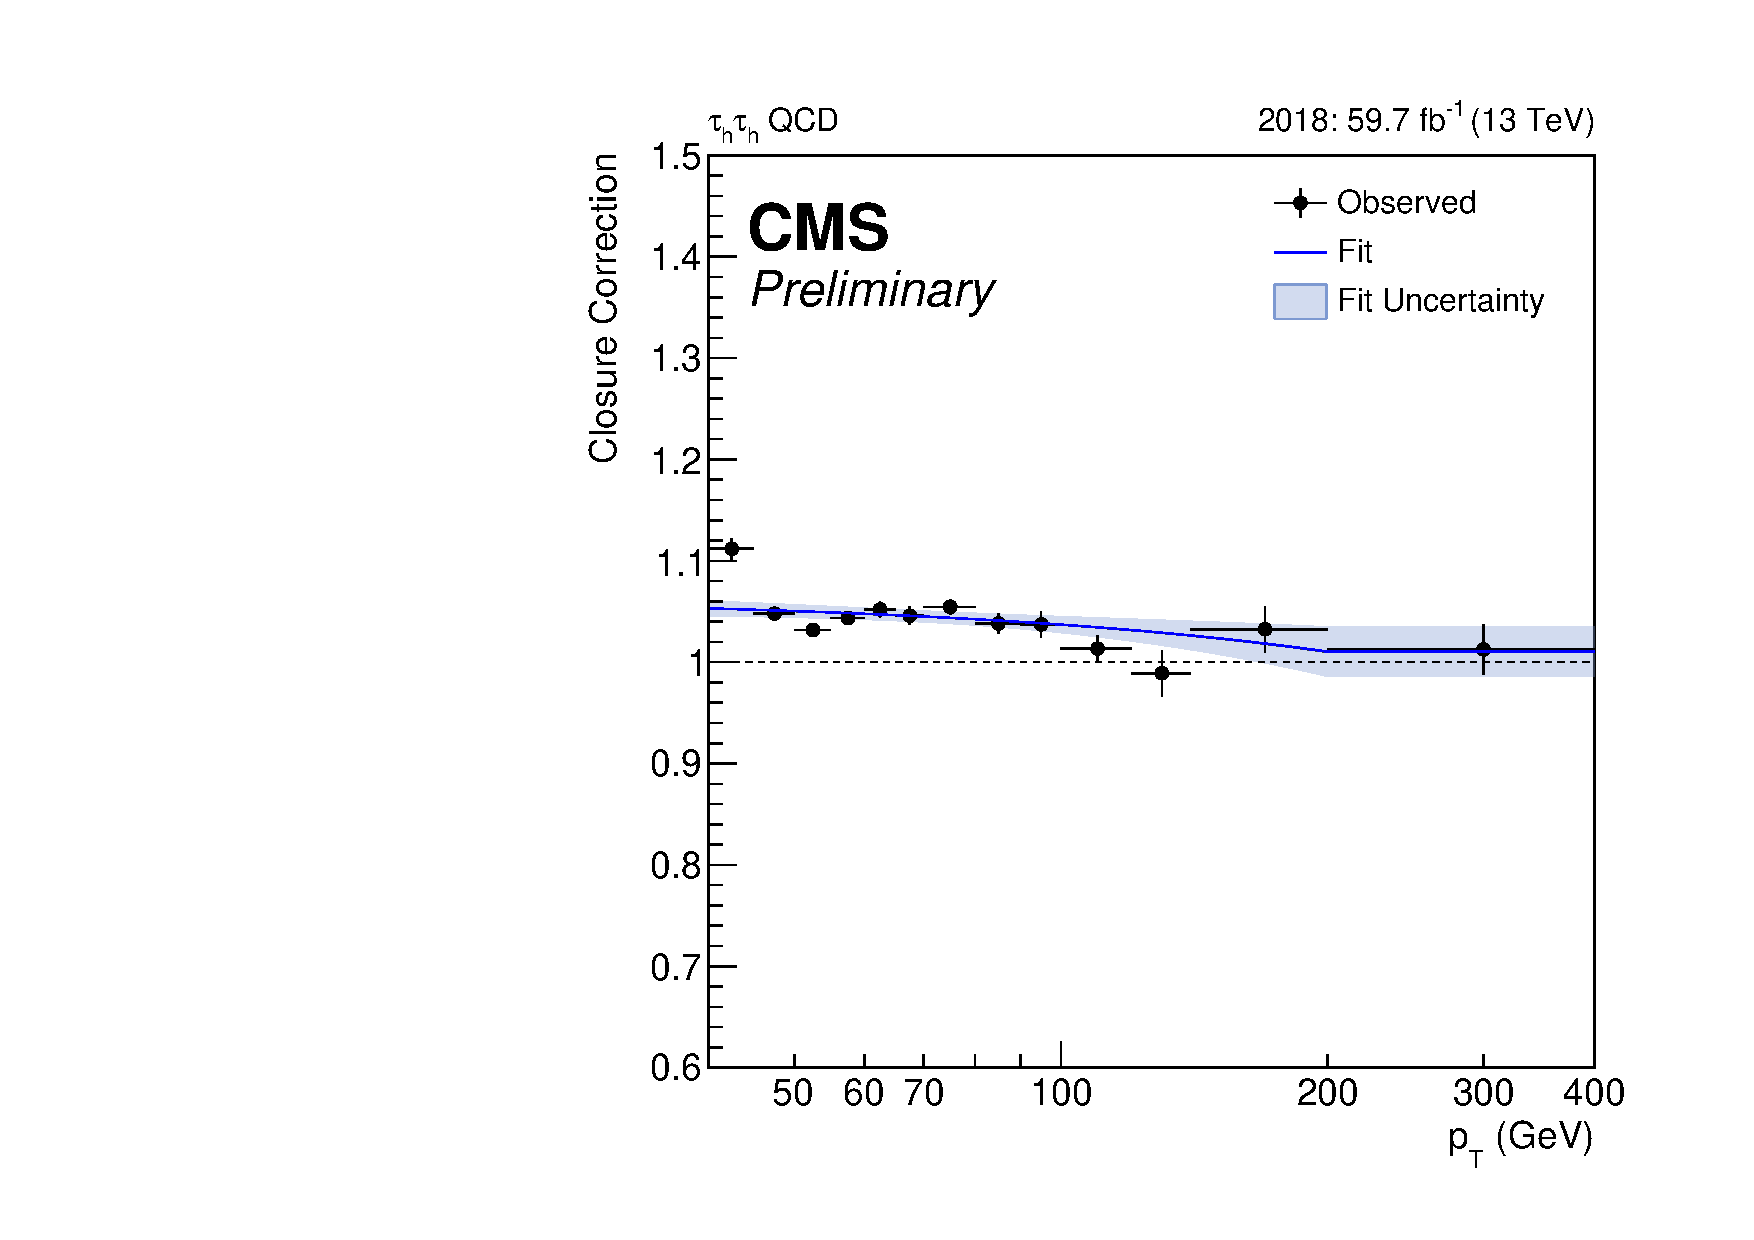
\includegraphics[width=0.33\textwidth]{Figures/ff_closure_os_closure_nbjet0_alt_qcd_tt_2018.pdf}} 
    \subfloat[]{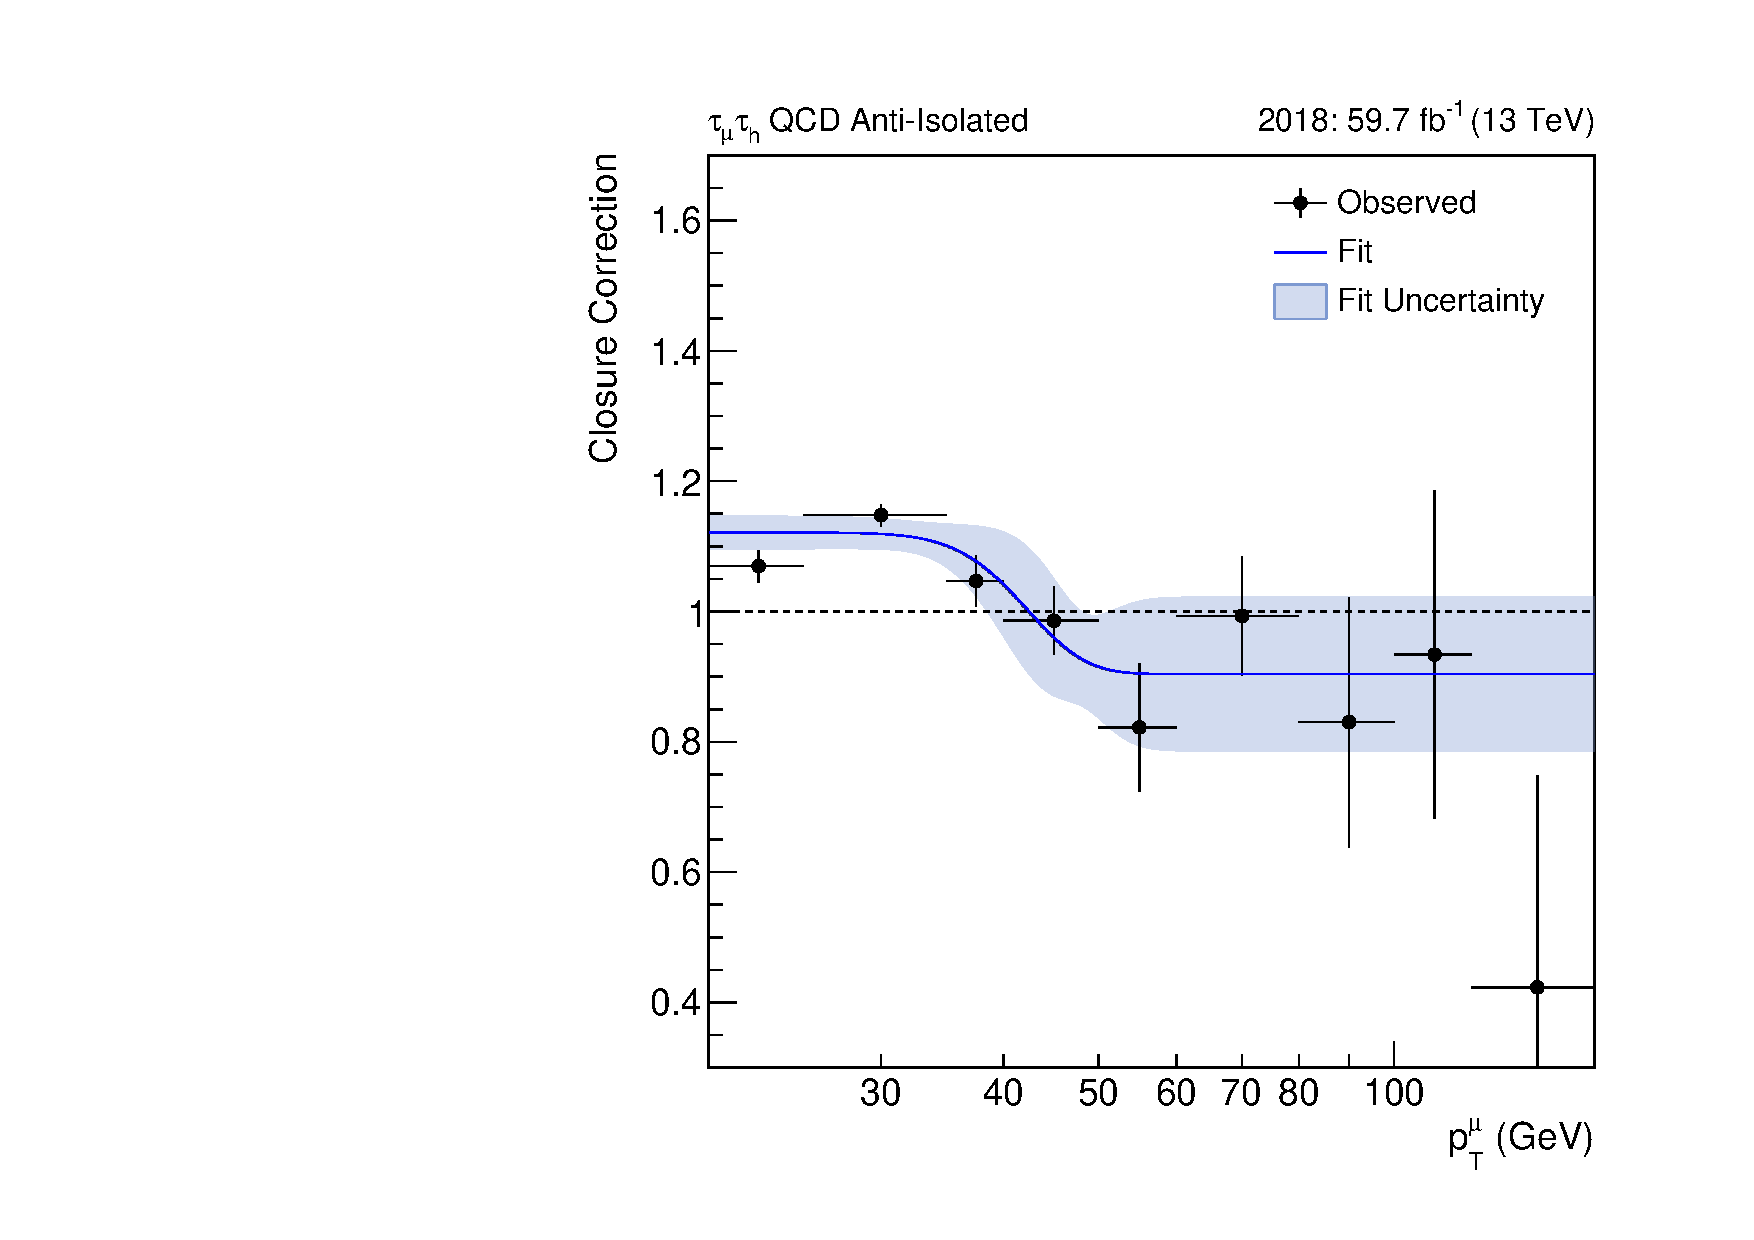
\includegraphics[width=0.33\textwidth]{Figures/ff_closure_pt_1_nbjets0_dr_to_ar_aiso_closure_qcd_mt_2018.pdf}}
    \subfloat[]{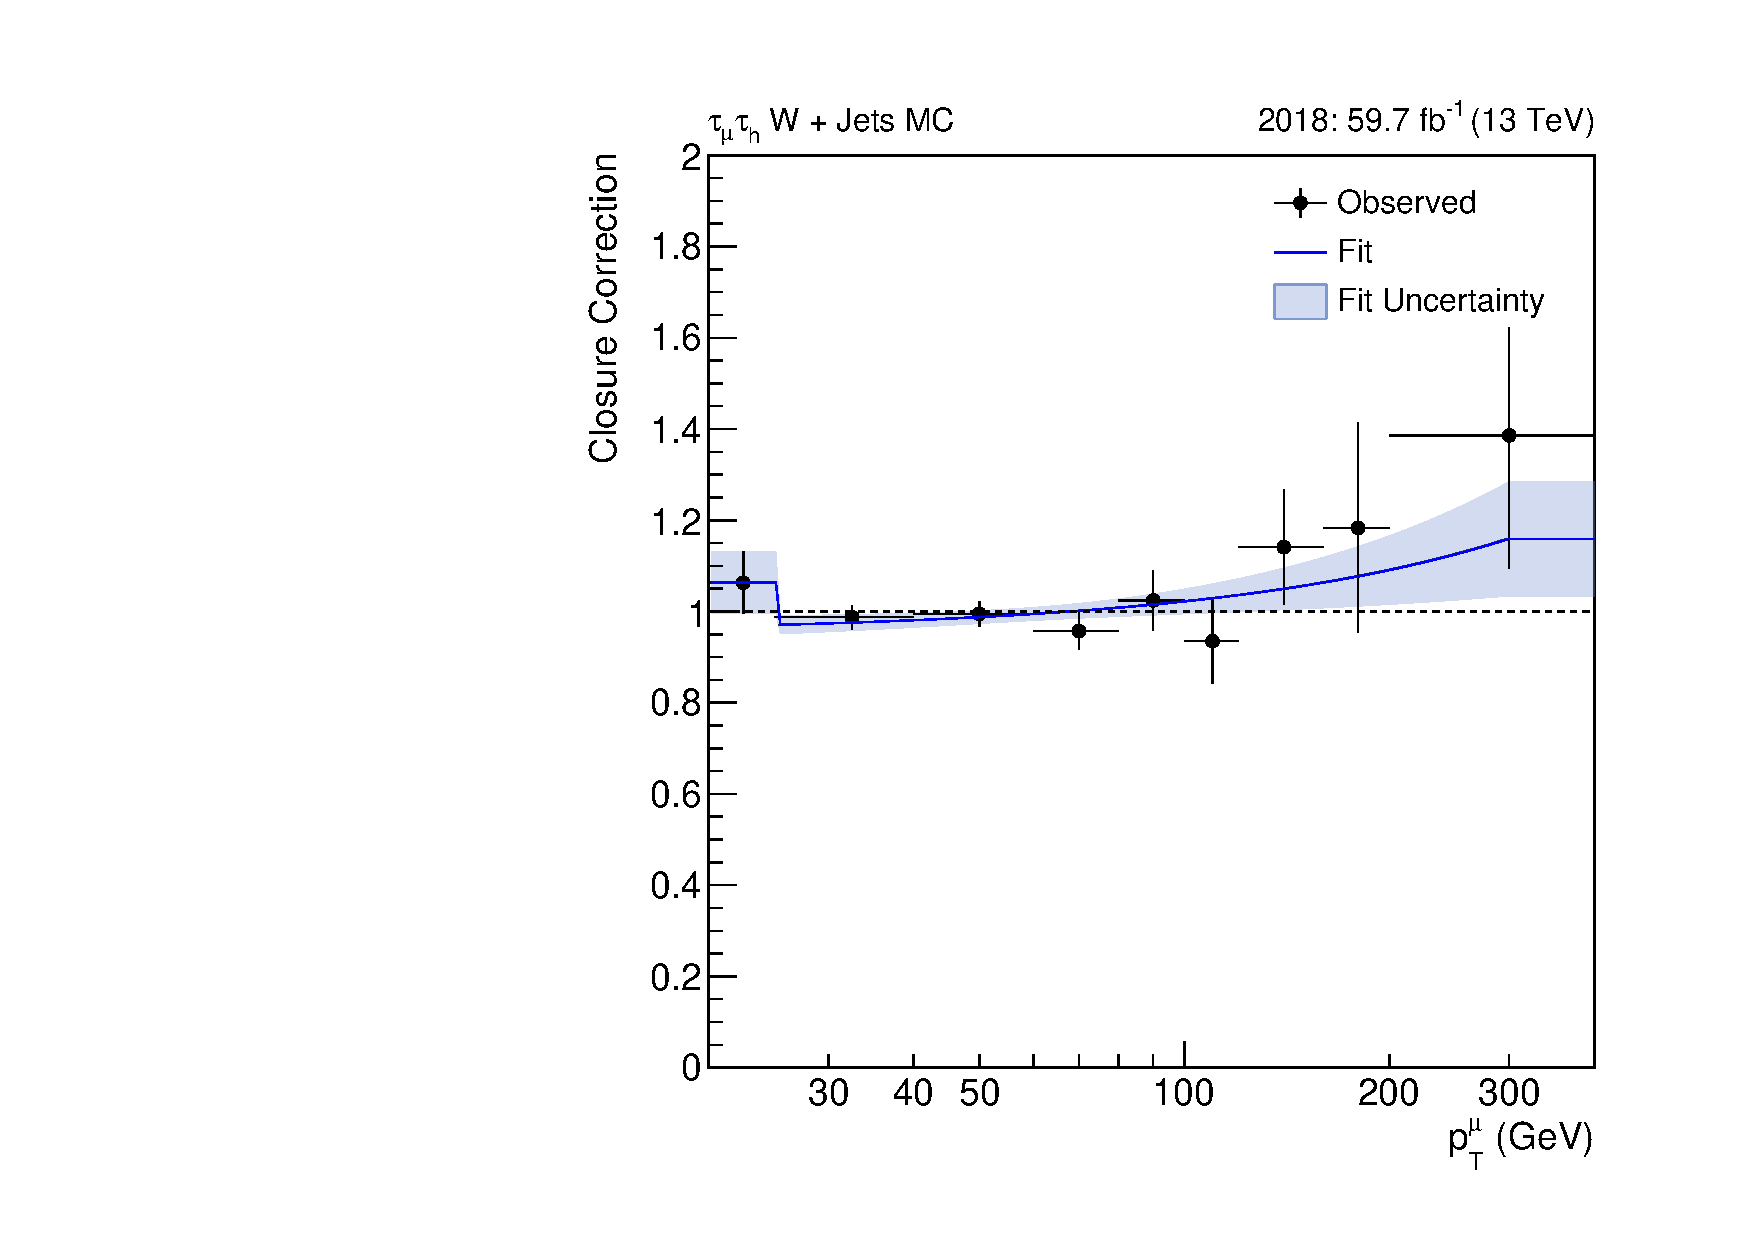
\includegraphics[width=0.33\textwidth]{Figures/ff_closure_pt_1_nbjets0_tightmt_dr_to_ar_closure_wjets_mc_mt_2018.pdf}}
\caption{Determination region to application region closure correction fits with 2018 data. (a) is the correction moving from same sign to opposite sign tau leptons the parameterised by leading $\tauh$ $\pT$ in events with $N_{\text{b-jets}}=0$ in the $\tauhtauh$ channel. (b) and (c) show the correction for the $\mutauh$ channel moving from same sign to opposite sign tau leptons and high $m_{T}$ to low $m_{T}$ both parameterised by the the muon $\pT$ for QCD and W + jets processes respectively.}
\label{fig:ff_dr_to_ar}
\end{figure}


\subsection{Applying Fake Factors}
\label{sec:ff_applying}

In the $\etauh$ and $\mutauh$ channels the $\FFi$ measured for the different processes are combined into an overall factor, $\FF$, using
\begin{equation}
\FF = \sum_{i}f_{i}\cdot \FFi,
\end{equation}
where the factor $f_{i}$ is defined as
\begin{equation}
f_{i} = \frac{N_{\text{AR}}^{i}}{\sum\limits_{j}N_{\text{AR}}^{j}},
\end{equation}
which is the fraction of events with a $\text{jet}\rightarrow\tauh$ originating from process $i$ over the total number of $\text{jet}\rightarrow\tauh$ events for all processes in the application region.
These fraction of events are estimated with MC, with a QCD model which is extrapolated from same sign tau pairs.
It is observed that W + jets is the dominating process in this region, however there are effect from QCD at low $\mT$ and from $\ttbar$ in the b tagged categories. These fractions are then multiplied to the relevant corrected fake factor and applied to the fail region in C, with any events which are not jets faking hadronic taus subtracted off with MC. \\

\begin{figure}[!hbtp]
\centering
    \subfloat[]{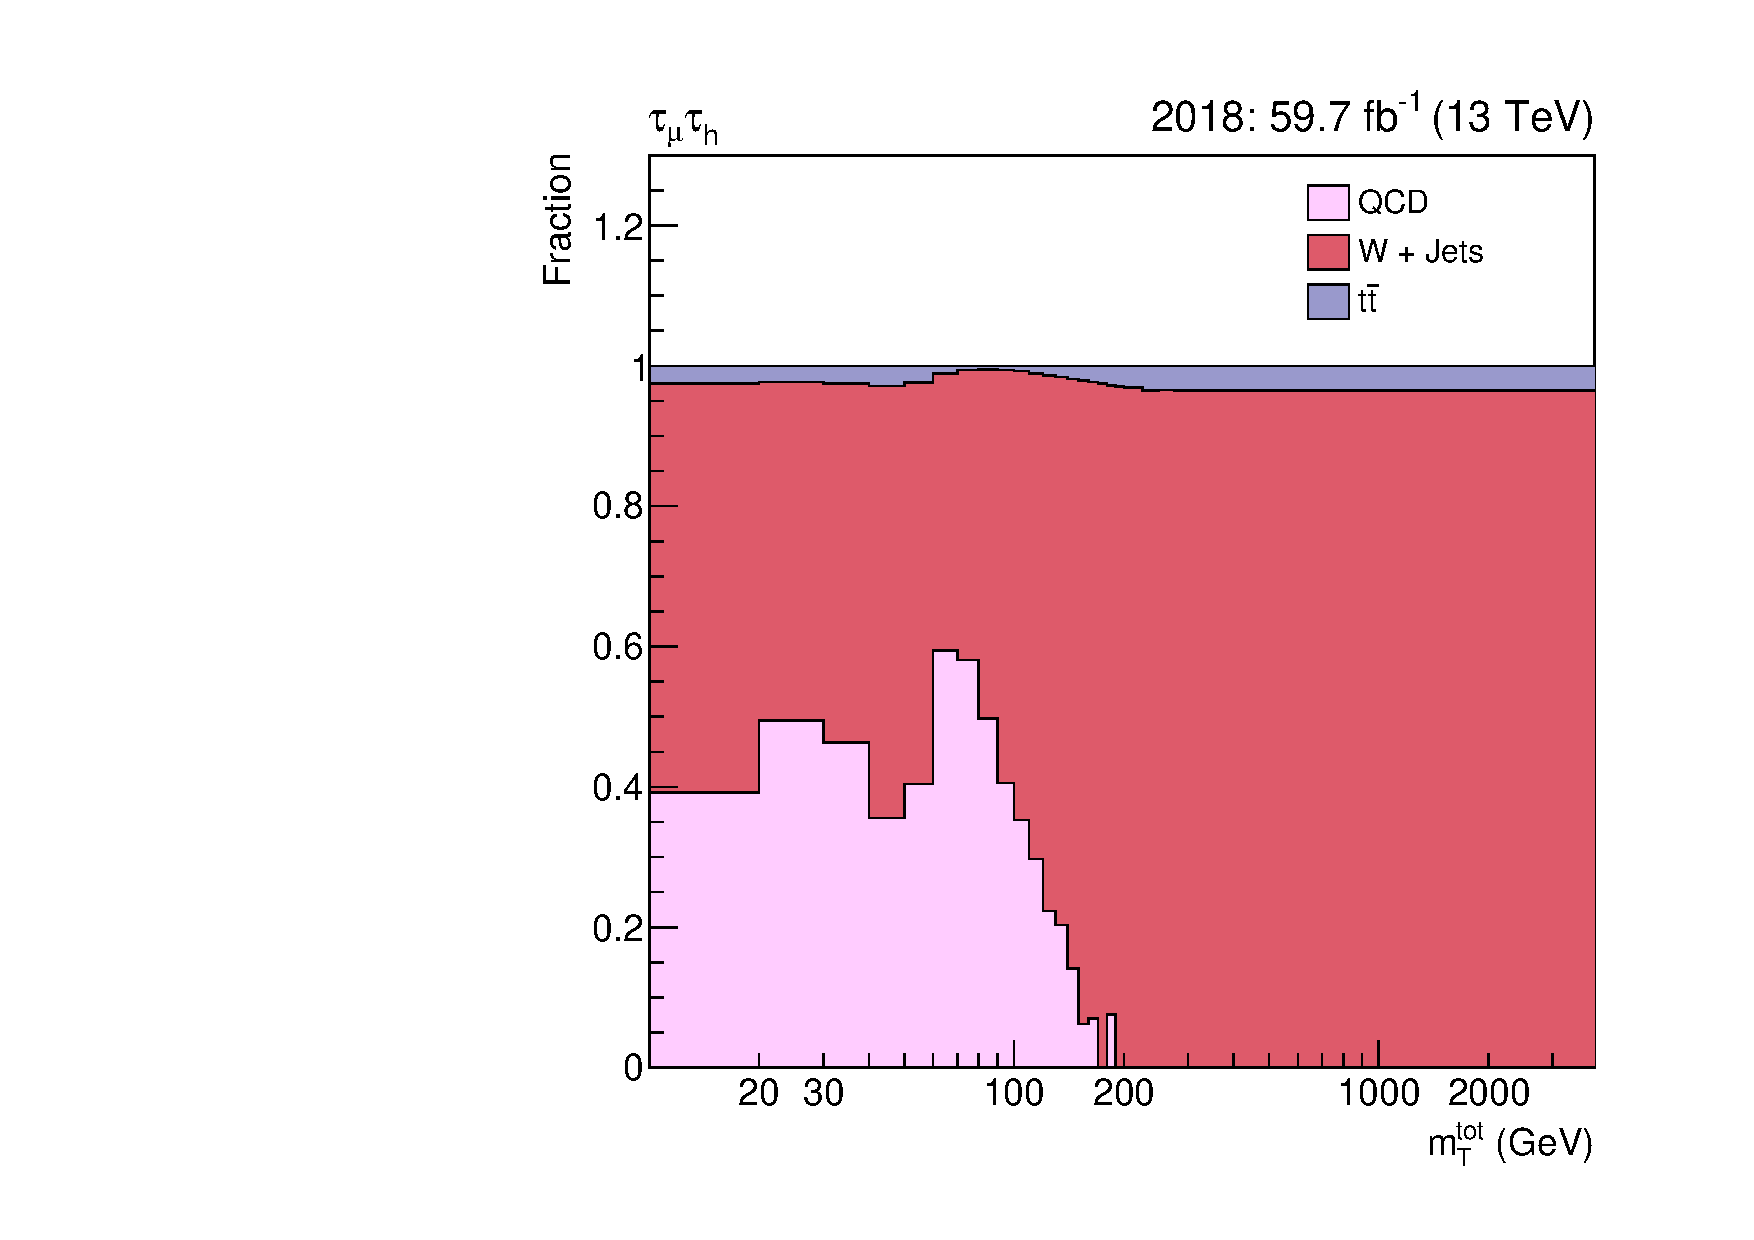
\includegraphics[width=0.45\textwidth]{Figures/ff_fraction_tightmt_nbjets0_mt_2018_os_rebinning.pdf}}
    \subfloat[]{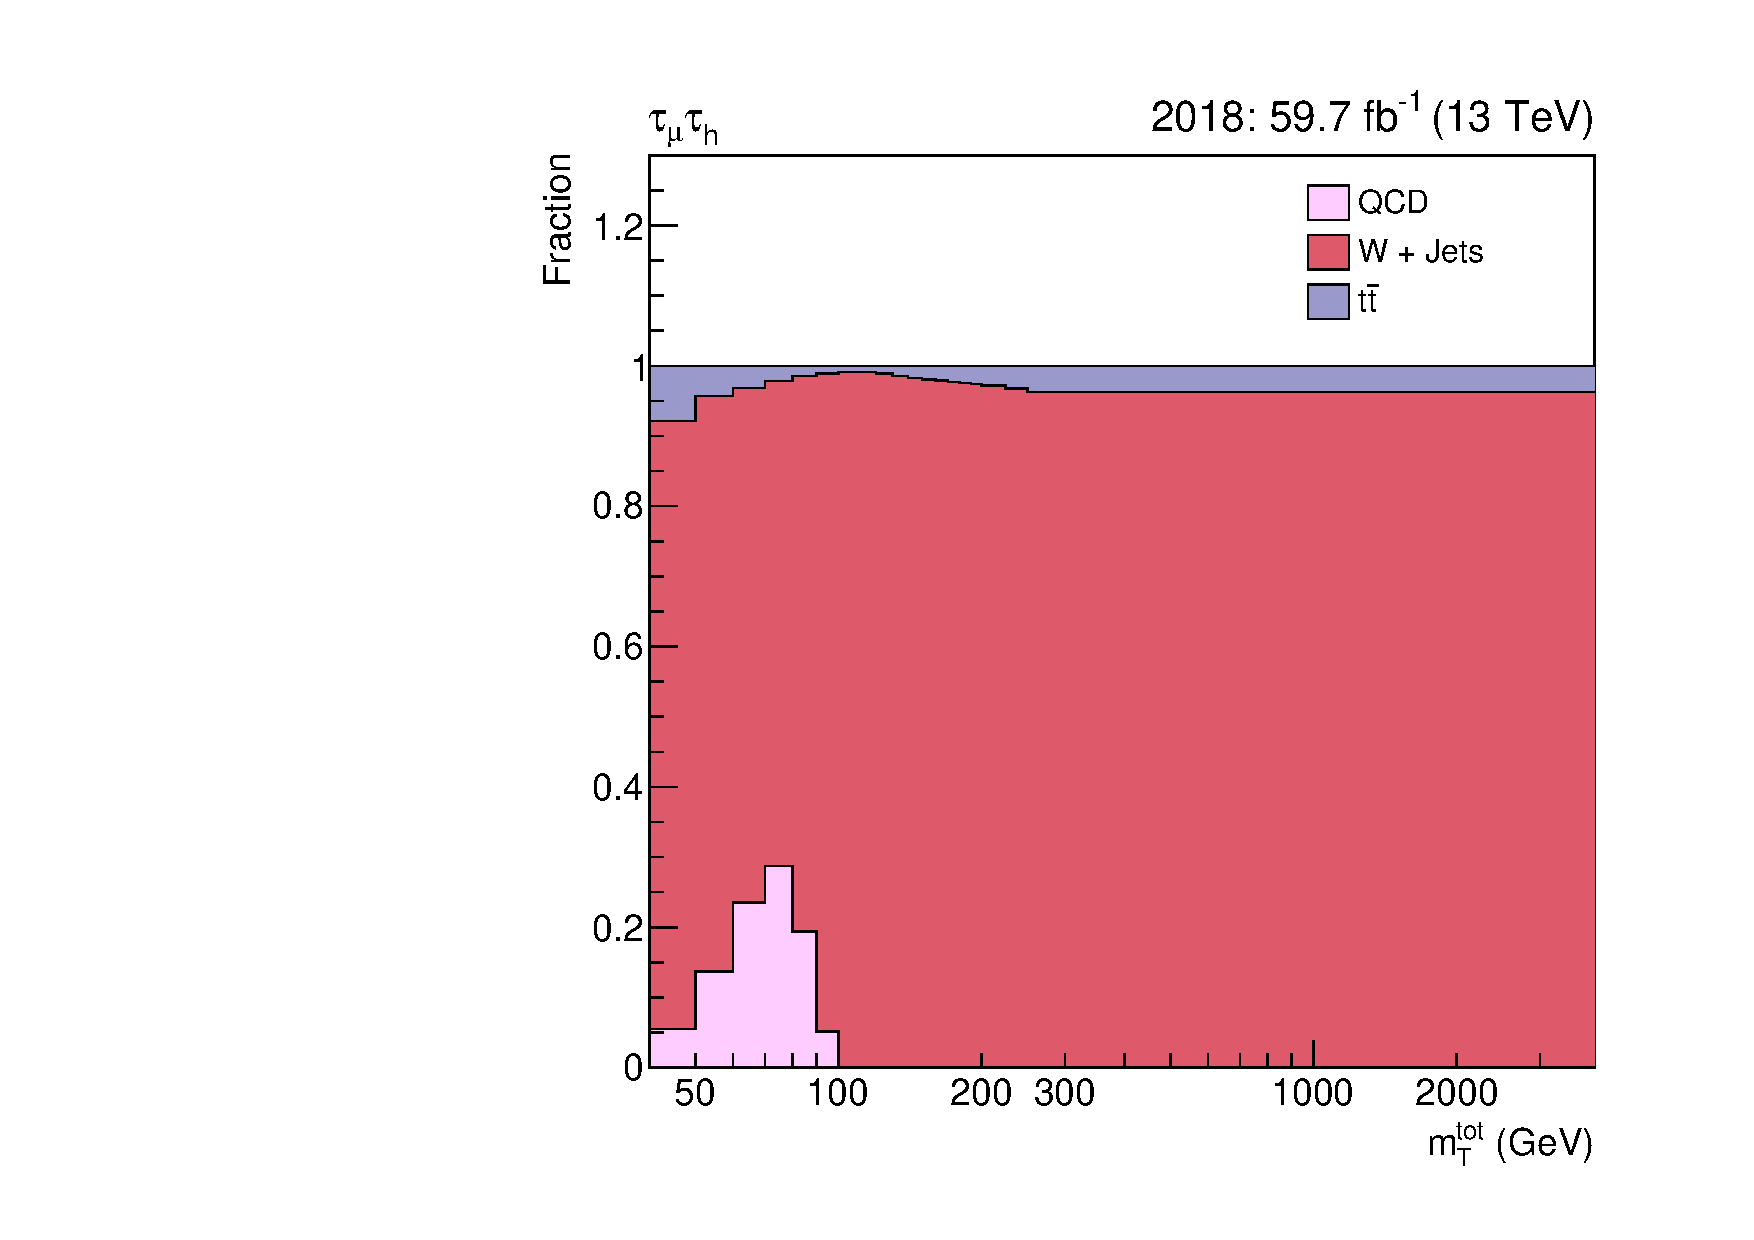
\includegraphics[width=0.45\textwidth]{Figures/ff_fraction_loosemt_nbjets0_mt_2018_os_rebinning.pdf}} \\
    \subfloat[]{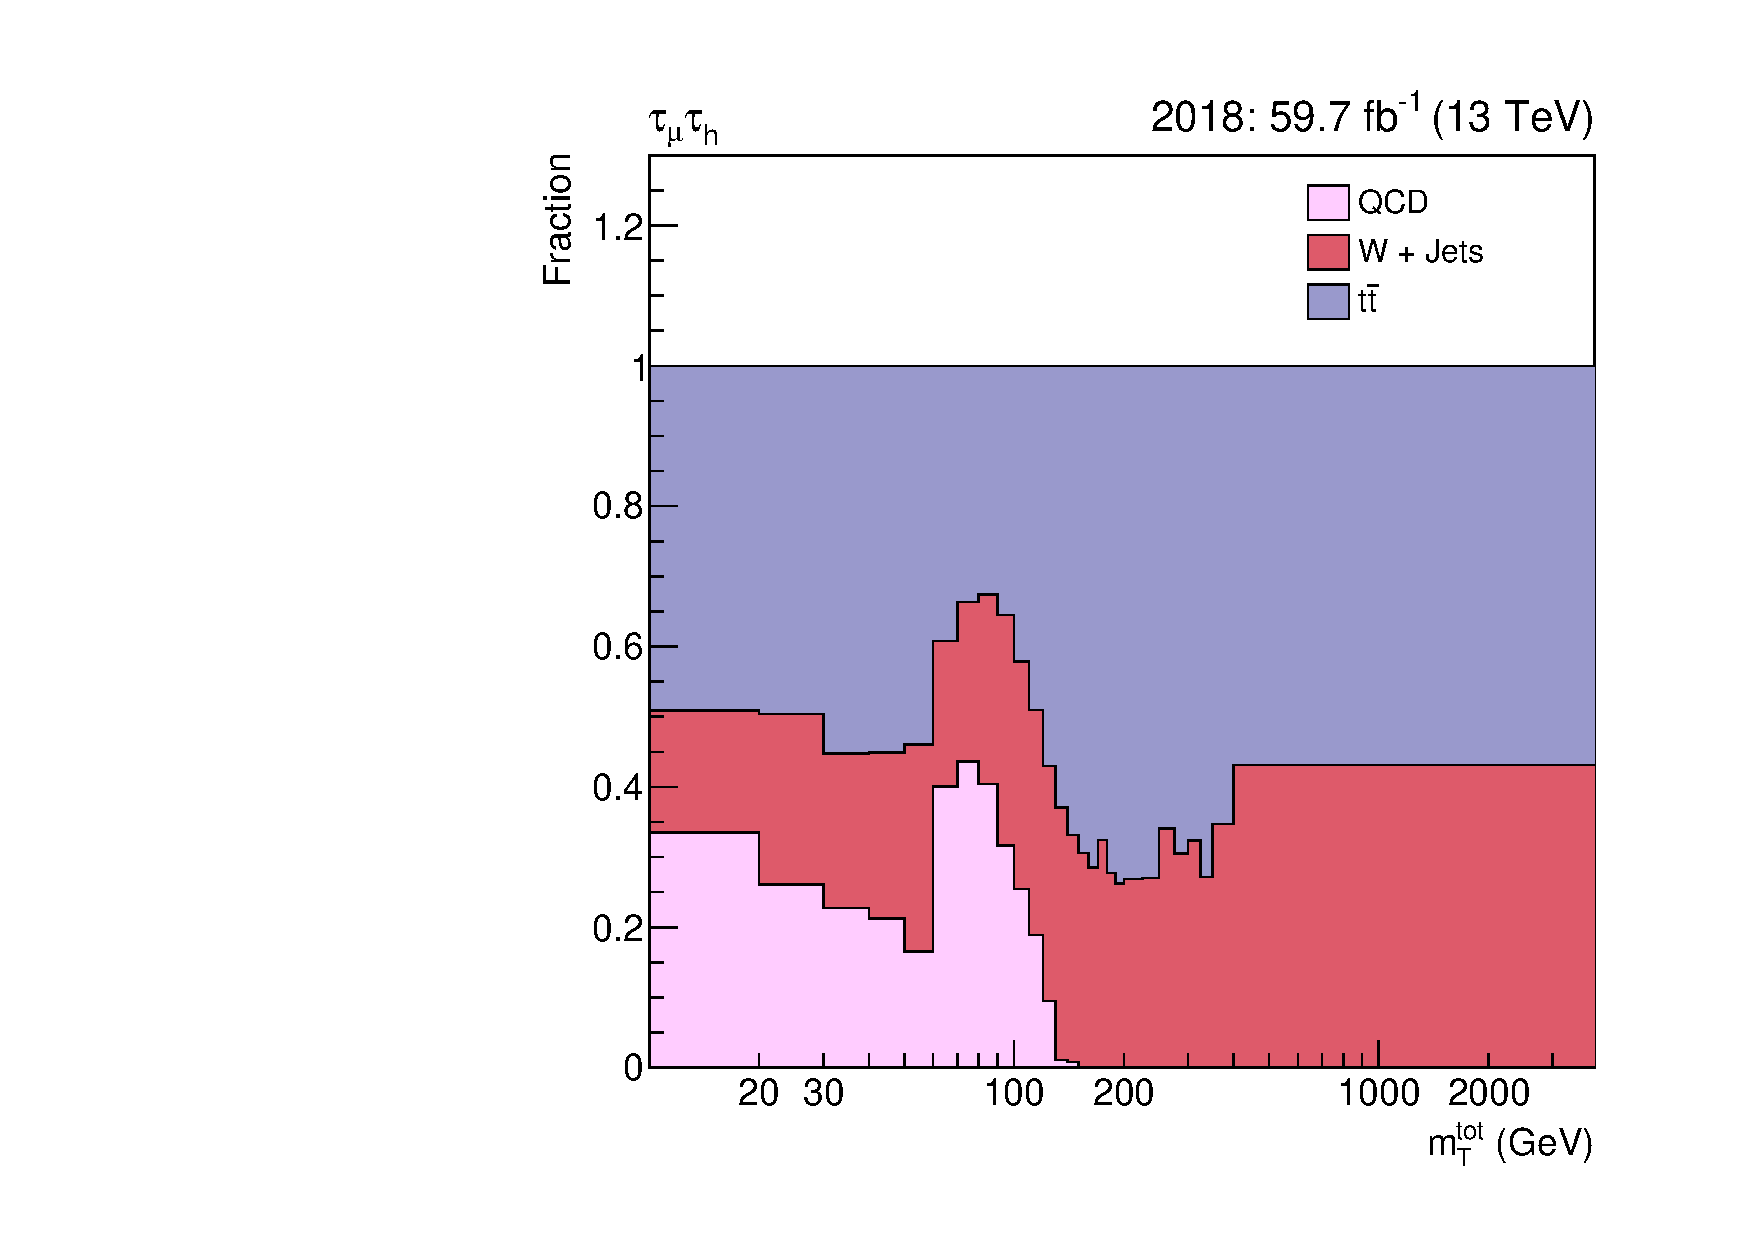
\includegraphics[width=0.45\textwidth]{Figures/ff_fraction_tightmt_nbjets1_mt_2018_os_rebinning.pdf}}
    \subfloat[]{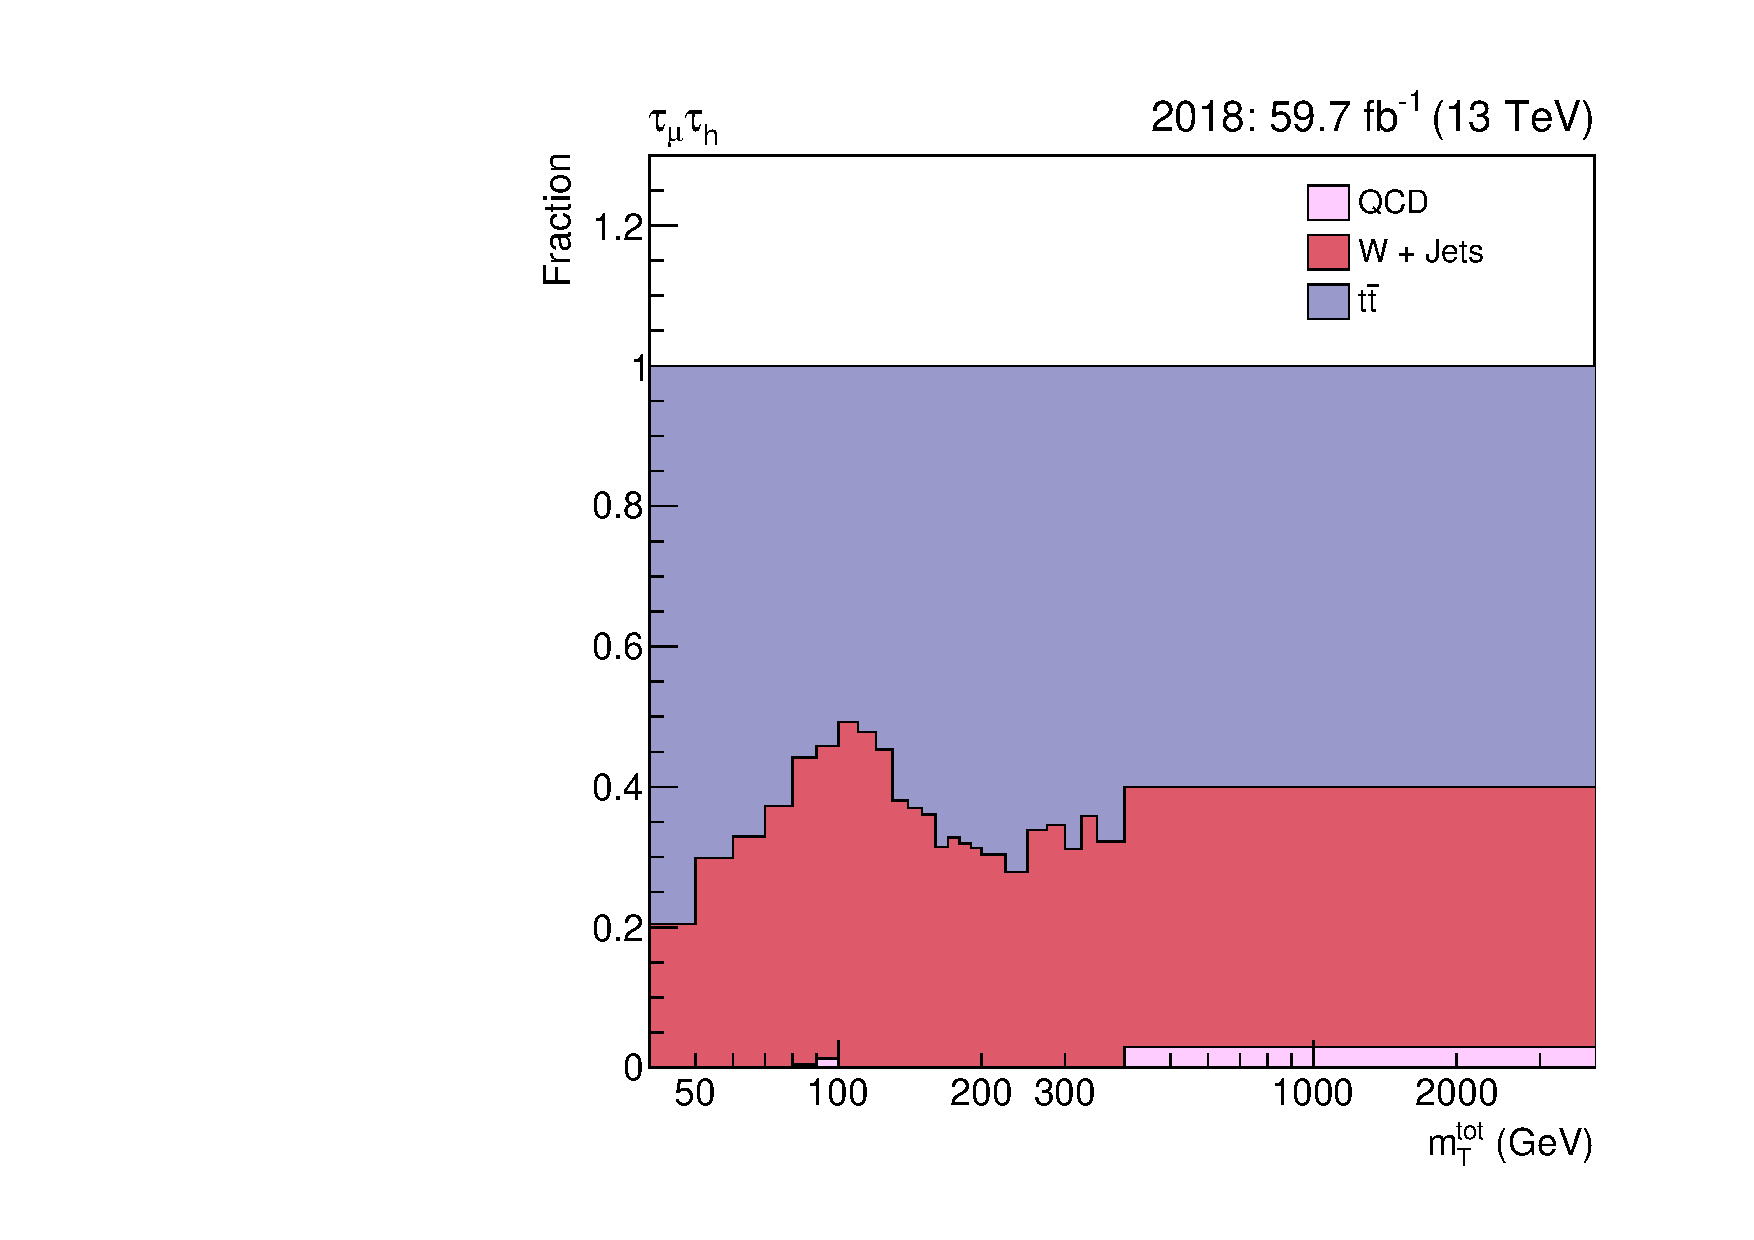
\includegraphics[width=0.45\textwidth]{Figures/ff_fraction_loosemt_nbjets1_mt_2018_os_rebinning.pdf}} \\
\caption{The expected application region fractions of the processes in the $\mutauh$ channel. (a) and (b) show the no b tag Tight-$m_{T}$ and Loose-$m_{T}$ categories and (c) and (d) show the b tag Tight-$m_{T}$ and Loose-$m_{T}$ categories respectively.}
\label{fig:mt_ff_frac}
\end{figure}

For the $\tauhtauh$ channel there are two hadronic taus that a jet can fake.
For this analysis, the fake factors are only applied the leading hadronic tau candidate failing the tau ID in C.
This models all events where the leading hadronic tau candidate is a jet fake.
However, this leaves a small fraction of events, where the leading candidate is a genuine tau and the sub-leading candidate is a jet fake.
This contribution (mostly from W + jets) is added back with MC.

\newpage
\section{MC Corrections}

\newpage
\section{Uncertainty Model}
\label{sec:uncerts}

The statistical uncertainties are taken into account by the Barlow-Beeston method, described in Ref.~\cite{}.
The systematic model is split into uncertainties based on the online and offline reconstruction of objects and the background and signal modelling.
An uncertainty is correlated across channels when it represents a shift on the reconstruction of an object and decorrelated otherwise.
It is decorrelated across era of data taking when the shift is derived independently by era.
The embedded samples use the same uncertainty scheme as MC but 50\% are correlated and 50\% uncorrelated with MC uncertainties, because of the shared real data in the measurement.

\subsubsection{Hadronic Taus}
Uncertainties on the tau triggers are obtained from the fitted scale factors used to derive the corrections for the tau trigger efficiencies.
The tau legs of the DoubleTau and lepton+tau cross triggers in different decay mode bins are treated as uncorrelated.
For the SingleTau trigger leg, due to limited statistics it is not possible to determine scale factors and uncertainties split by decay mode and therefore a single uncertainty common to all decay modes is applied.
The DoubleTau trigger uncertainties are further split the hadronic trigger efficiencies in the $\pT$ regions $<$ 100 GeV and $>$ 100 GeV to allow the fit more freedom to adjust the high $\pT$ regions relative to the low $\pT$ regions.
Uncertainties are also applied on the energy scale of the hadronic taus. 
These uncertainties range between 0.2 and 1.1 \%. 
Finally, an uncertainty on the ID efficiency is placed as a function of $\pT$ in the $\etauh$ and $\mutauh$ channels, and of the tau decay mode in the $\tauhtauh$ channels. 
These vary between 3-9\% and is uncorrelated in each variable bin it is derived in.
To account for the different anti-lepton discriminator working points, an uncertainty of 3\% per tau is applied and treated as uncorrelated between the channels where different $D_{\text{WP}}^{e/\mu}$ are used.

\subsubsection{Light leptons}
The uncertainty on the trigger efficiencies amounts to 2\% per lepton in the $\etauh$, $\mutauh$ and $\emu$ channels.
They are basically normalisation uncertainties but implemented as shape uncertainties as they only touch the events triggered by the corresponding cross trigger or single lepton triggers.
Uncertainties are also placed on the electron energy scale based off the calibration of ECAL crystals.
This information is not reliable for embedding samples and so uncertainties of 0.5-1.25\% are placed here. 
The energy scale variations are negligible and so not included.
Another 2\% uncertainty is placed on the ID of any electron or muon in the event.

\subsubsection{Jets}
Jet energy scale and resolution uncertainties arise from a number of sources. 
These include limited statistical measurements used for calibration, energy measurement changes due to detector ageing, and bias corrections to address differences between simulation and data. 
Uncertainty ranges are from sub-percent to \order(10\%).
Uncertainties are also placed on the tagging of b jets, which vary from 0--3\%.

\subsubsection{Leptons misidentified as hadronic taus}
Uncertainty shifts are applied for the energy scale of leptons faking hadronic taus parametrised by the $\pT$ of the $l \rightarrow\tauh$ fake.
The magnitude is 1.0\% for muons in all eras and for electrons the uncertainties vary between 0.5 and 6.6 \%.

\subsubsection{Jets misidentified as hadronic taus}
The backgrounds with jets misidentified as $\tauh$ are estimated from data with the fake factor method. 
There are different sources of uncertainty related to this method.
The first uncertainties come from subtracting off other background processes with MC to form the determination region. 
The subtraction is shifted up and down by 10\% to determine new weights.
Next, statistical uncertainties on all of the fake factor method fits are accounted for, where the binned values are uncorrelated with the rest of the fit.
An uncertainty is also placed on the choice of fit function, the shifts are estimated by comparing the fits to a 1st order polynomial fit set to constant above 100 GeV.
The final systematic variation are then on the extrapolation corrections by applying the corrections twice and not at all.
The size of each systematic uncertainty varies from 0--10\%, whilst the statistical element from the fits can be larger in the tails of the distributions.

\subsubsection{MET}
The MET uncertainties is different dependent on process.
For all processes that are not $\ttbar$ and diboson, the hadronic recoil response and its resolution are varied within the uncertainties determined during the computation of the recoil corrections.
For $\ttbar$ and diboson an uncertainty is derived on the energy carried by an unclustered particle \cite{}.
These uncertainties vary between 0--10\%.

\subsubsection{Background process specific uncertainties}
Uncertainties on the $\ttbar$ $\pT$ and DY $m_{ll}$-$\pT$ reweighting is placed by the applying the correction twice and not at all.
An additional uncertainty is placed to cover the $\ttbar$ contamination in embedding, where the removed $t\bar{t}$ genuine tau pair is shifted up and down by 10\%.
Some non-closures are observed in embedded $Z\to\mu\mu$ control samples. 
Therefore, these non-closures are taken as an additional shape uncertainty as a function of the Z $\pT$ and $m_{\tau\tau}$.

\subsubsection{Signal process specific uncertainties}
For the gg$\phi$ process, in particular for low mass hypotheses, the variation of \texttt{hdamp} parameter of the \POWHEG MC generator as well as the $\mu_{R}$/$\mu_{F}$ scale variations are used to determine the uncertainties
on the $\pT$ spectrum of each contribution at NLO QCD to the Higgs boson production via gluon fusion (top, bottom, top-bottom interference). These are also determine from additional samples produced
up to the generator level, and applied as event weights dependent on generator level $\pT$ after the parton shower simulation. These uncertainties are included as shape uncertainties as they may affect the shapes of the $m_{T}^{\text{tot}}$ distribution as well as the predicted signal yields.

\subsubsection{Luminosity}
($1.2\,\%$, $2.3\,\%$, $2.5\,\%$) normalisation luminosity uncertainty is applied to the (2016, 2017, 2018) templates which originate from MC simulation.

\subsubsection{Prefiring}
Upper and lower bounds are taken from the efficiency maps provided by the L1 DPG and propagated on all MC samples as shape uncertainty for 2016 and 2017.
The size of the uncertainty as the weight itself depends on the event topology. In general the uncertainty is at the order of 1\%.

\newpage
\section{Signal Extraction}
\label{sec:sig_ext}

A simultaneous binned maximum likelihood fit over all analysis categories is used to extract the results.
The likelihood take the form,
\begin{equation}
\mathcal{L}(\text{data}\mid\mu,\theta) = \prod_{i}^{N_{i}} \text{Poisson} \Big(n_{i} \mid \sum_{j}^{N_{j}} g_{j}(\mu_{ij}) \cdot s_{ij}(\theta) + \sum_{k}^{N_{k}} b_{ik}(\theta)\Big) \cdot p(\hat{\theta} \mid \theta),
\label{eqn:likelihood}
\end{equation}

where $i$ loops through all histogram bins and analysis categories.
$j$ and $k$ loop over all signal and background processes of the hypothesis being fit.
$n_i$, $s_i$ and $b_i$ are the data observed, signal and background expectation respectively in each bin.
$\theta$ represents the set of nuisance parameters (corresponding to the systematic uncertainties as detailed in Section~\ref{sec:uncerts}) that parametrise the signal and background modelling.
$\mu$ are rate parameters and $g(\mu)$ are scaling functions that scale to a signal to a signal hypothesis.
The form of the Poisson probabilities are,
\begin{equation}
\text{Poisson} (n \mid x) = \frac{x^{n}e^{-x}}{n!}.
\end{equation}
Finally, $p(\hat{\theta} \mid \theta)$ represents the probability density function (pdf) of each nuisance parameter ($\theta$) with respect to the initial value of the parameter ($\hat{\theta}$). \\

These come in two forms, the first is for uncertainties that only affect the normalisation of the process and are modelled by log-normal pdfs. 
The second is for uncertainties that affect the shape of the distribution, these are assigned Gaussian pdfs.
The $\pm1\sigma$ shifts for each shape variations are derived and vertical morphing \cite{} is used to interpolate and extrapolate within and outside the shifts.
Both pdfs are depend on the mean ($\mu$) and standard deviations ($\sigma$) and the functional forms are shown in Table~\ref{tab:pdfs}. \\

\begin{table}[!hbtp]
    \centering
    \begin{tabular}{|c|c|}
         \hline
         Gaussian & Log-normal  \\
         \hline
         \hline
          & \\
         $f(x) = \frac{1}{\sqrt{2\pi\sigma^{2}}} \exp\Big({-\frac{(x - \mu)^2}{2\sigma^2}}\Big)$ & $f(x) = \frac{1}{x} \frac{1}{\sqrt{2\pi\sigma^{2}}} \exp\Big({-\frac{(\ln x - \mu)^2}{2\sigma^2}}\Big)$ \\
          & \\
         \hline
    \end{tabular}
    \caption{pdfs used for nuisance parameters.}
    \label{tab:pdfs}
\end{table}

The following subsections discuss the results of many such fits.
The key fits to understand the results are the background-only fit and the signal-plus-background fits.
It is important to mention here that the SM Higgs boson processes are treated as a background.
The background-only fit is performed with $N_j$ (number of signal processes) set to 0.
For all signal-plus-background fits, the fit is done with respect to a single mass hypothesis, however within this mass hypothesis can be a number of signal processes.
The model independent resonance search has separate $gg\phi$ and $bb\phi$ signal modes and so two rate parameters $\mu_{gg\phi}$ and $\mu_{bb\phi}$ are needed.
When the samples are originally scaled to the cross section times branching ratio ($\sigma \times B (\phi\rightarrow\tau\tau)$) of 1 pb and $g(\mu)=\mu$ for both processes, $\mu_{gg\phi}$ and $\mu_{bb\phi}$ represent the $\sigma \times B (\phi\rightarrow\tau\tau)$ with units of pb.
To avoid negative signal strengths, $\mu$ will only be taken to be positive.
Also used in the following subsections, is a signal-plus-background channel/category compatibility fit.
In this fit the signal processes and rate parameters are further split in each channel or category utilising index $i$ in Eq.~\ref{eqn:likelihood}.
This is used to determine the compatibility of the results in different decay channels and analysis categories.
In this case, $\mu$ is allowed to take negative values to help fully understand the fits to data in each channel or category. \\

The vector leptoquark search has two signal modes; the t-channel interaction and the interference with Drell-Yan however as this is a model dependent interpretation of these results both these rate parameters scale together.
The scaling functions differ between the two processes with $g_{\text{t-channel}}(\mu) = \mu^4$ and $g_{\text{interference}}(\mu) = \mu^2$ to mimic how the cross sections of each process scales.
When the initial samples are scaled to cross section at $g_{U}=1$, $\mu$ corresponds to the coupling $g_{U}$. \\

For the MSSM interpretation of the results, there are three Higgs bosons to consider in the signal model (h, H and A) produced via both gluon fusion and in association with b quarks.
The gluon fusion samples are also split into the separate loop contributors, so the kinematic properties can be properly scaled to MSSM prediction, as described in Section~\ref{sec:additional_higgs_bosons}.
The SM-like Higgs boson is considered in the MSSM signal model to monitor differences in the observed Higgs boson prediction between the MSSM and the SM.
In each benchmark scenario chosen, the signal prediction depends only on $m_{A}$ and $\tan\beta$ and the scaling to cross section is shown in Eq.~\ref{eqn:mssm_xs}.
As the potential scaling functions for MSSM interpretations are not necessarily smooth one-to-one mappings, the likelihood is tested for individual points on the $m_{A}$-$\tan\beta$ parameter space.
At each point, the MSSM Higgs bosons are scaled to the theory predicted cross section times branching ratio.
To test the MSSM hypothesis over the SM hypothesis, the single rate parameter $\mu$ is used and only allowed to take values of 1 (MSSM) and 0 (SM) with $g(\mu)=\mu$.
As the SM Higgs boson is added to the background modelling and the MSSM prediction of the observed Higgs boson is added to the signal model when $\mu=1$, the SM Higgs boson prediction must then be subtracted from the signal model. \\

The confidence intervals in the best fit results are given by the $-2\Delta\ln\mathcal{L}$, where $\Delta\ln\mathcal{L}$ is the difference between $\ln\mathcal{L}$ of the best fit model and the test value of $\mu$. 
The 68\% and 95\% confidence regions with two degrees of freedom (as in the model independent resonant search) are determined by $-2\Delta\ln\mathcal{L} = 2.28$ and $5.99$ respectively. \\

Upper limits are placed using the modified frequentest approach \cite{} with profile likelihood ratio used for the test statistic defined below.
\begin{equation}
  q_{\mu} = -2 \ln \Biggl(\frac{\mathcal{L}(\text{data} | \mu, \hat{\theta}_{\mu})}{\mathcal{L}(\text{data} | \hat{\mu}, \hat{\theta}_{\hat{\mu}})}\Biggl), 0 \leq \hat{\mu} \leq \mu,
\end{equation}
where $\hat{\mu}$ and $\hat{\theta}_{\hat{\mu}}$ are the best fit values of $\mu$ and $\theta$. $\hat{\theta}_{\mu}$ are the values of $\theta$ that is maximised by the likelihood for a tested value of $\mu$.
The bounds on $\hat{\mu}$ are to ensure a positive signal strength with a one-sided confidence interval.
The probability of $q_{\mu} \geq q_{\mu}^{\text{obs}}$ is,
\begin{equation}
\text{CL}(\mu) = \int^{\infty}_{q_{\mu}^{\text{obs}}} f(q_{\mu} \mid \mu, \theta_{\mu}^{\text{obs}}),
\end{equation}
where $f(q_{\mu} \mid \mu, \theta_{\mu}^{\text{obs}})$ is the pdf of $q_\mu$.
$\text{CL}_{b}$ and $\text{CL}_{s+b}$ are then defined by the relevant background-only and signal-plus-background fits.
$\text{CL}_s$ is defined as the ratio of $\text{CL}_{s+b}$ and $\text{CL}_{b}$ and then upper limits are placed at the confidence level of $1-\text{CL}_{s}$.
The $f(q_{\mu} \mid \mu, \theta_{\mu}^{\text{obs}})$ are determined using the asymptotic approximation \cite{} and results are cross-checked and deemed consistent with toy MC datasets. \\

If a deviation from the background expectation is observed, the size of the deviation is quantified by a significance.
To begin quantifying the excess, a $p$-value is determined, $\mu$ is replaced with 0 in the test statistic, to test rejection of the background-only hypothesis in favour of the signal-plus-background hypothesis.
The $p$-value, $p_0$ is then,
\begin{equation}
p_{0} = \int^{\infty}_{q_{0}^{\text{obs}}} f(q_{0} \mid 0, \theta_{\mu}^{\text{obs}}).
\end{equation}
$p_{0}$ is uniformly distributed between 0 and 1 for the background-only hypothesis and so the probability and significance of rejecting the background-only hypothesis can be found. \\
 
\newpage
\section{Postfit Plots}

Figures~\ref{fig:low_mass_postfit} and \ref{fig:high_mass_postfit} show the unblinded distributions in the most sensitive analysis categories.
For simplicity, the $\etauh$ and $\mutauh$ channels have been combined.
Figure~\ref{fig:low_mass_postfit} shows the distributions of the $m_{\tau\tau}$ discriminator in the no b tag low mass optimisation categories. 
A signal-plus-background fit for a model independent gluon fusion resonant mass hypothesis of 100 GeV is shown and the changes in the background modelling when using a background-only fit is displayed in the ratio.
Figure~\ref{fig:high_mass_postfit} shows the distributions of the $m_{T}^{\text{tot}}$ discriminator in the high mass optimisation categories.
A background-only fit is shown for the stacked background and best fit signal hypotheses for the model independent resonances gg$\phi$ and bb$\phi$ 1.2 TeV and VLQ (BM 1) 1 TeV mass points from separate signal-plus-background fits are displayed. \\

In the low mass optimisation categories, a small excess of events is observed on the Z boson peak in the no b tag categories and reasonable agreement is observed in the b tag categories.
The excess of events are distributed in $m_{\tau\tau}$ between 80 and 120 GeV.
A signal-plus-background hypothesis is best fit with a 100 GeV gg$\phi$ with a cross section times branching ratio of 5.8 pb. 
In this same fit the bb$\phi$ process is constrained by the b tag categories to give a signal yield of 0.
A background-only fit is also performed on the data, it is observed that this can only partly explain the differences observed between background and data.
Even after a background-only fit there is still an small excess of data events over the Z boson peak. \\

In the high mass optimisation categories, another small excess is observed in high $m_{T}^{\text{tot}}$ bins, particularly in the most sensitive no b tag categories.
This excess is best fit by a model independent gluon fusion resonant mass at 1.2 TeV with a cross section times branching ratio of 3.1 fb.
There are no considerable differences observed in background modelling between signal-plus-background and background-only fits.
This is as the uncertainties in these bins are more statistically dominated and the majority of the systematic uncertainties are constrained in the bulk of the distribution.
Good agreement is observed in the rest of the distribution.
There is a very small deviation in the b tag categories, but as this can also be explained by a gg$\phi$ signal, the bb$\phi$ signal is heavily constrained and so largely does not contribute to the signal-plus-background fit of the excess.
Similar to the bb$\phi$ signal, the VLQ BM 1 signal is constrained by the results in the no b tag categories, leading to a non-zero best fit signal strength, but cannot explain the excess in the no b tag categories. \\

\begin{figure}[!hbtp]
\centering
    \subfloat[]{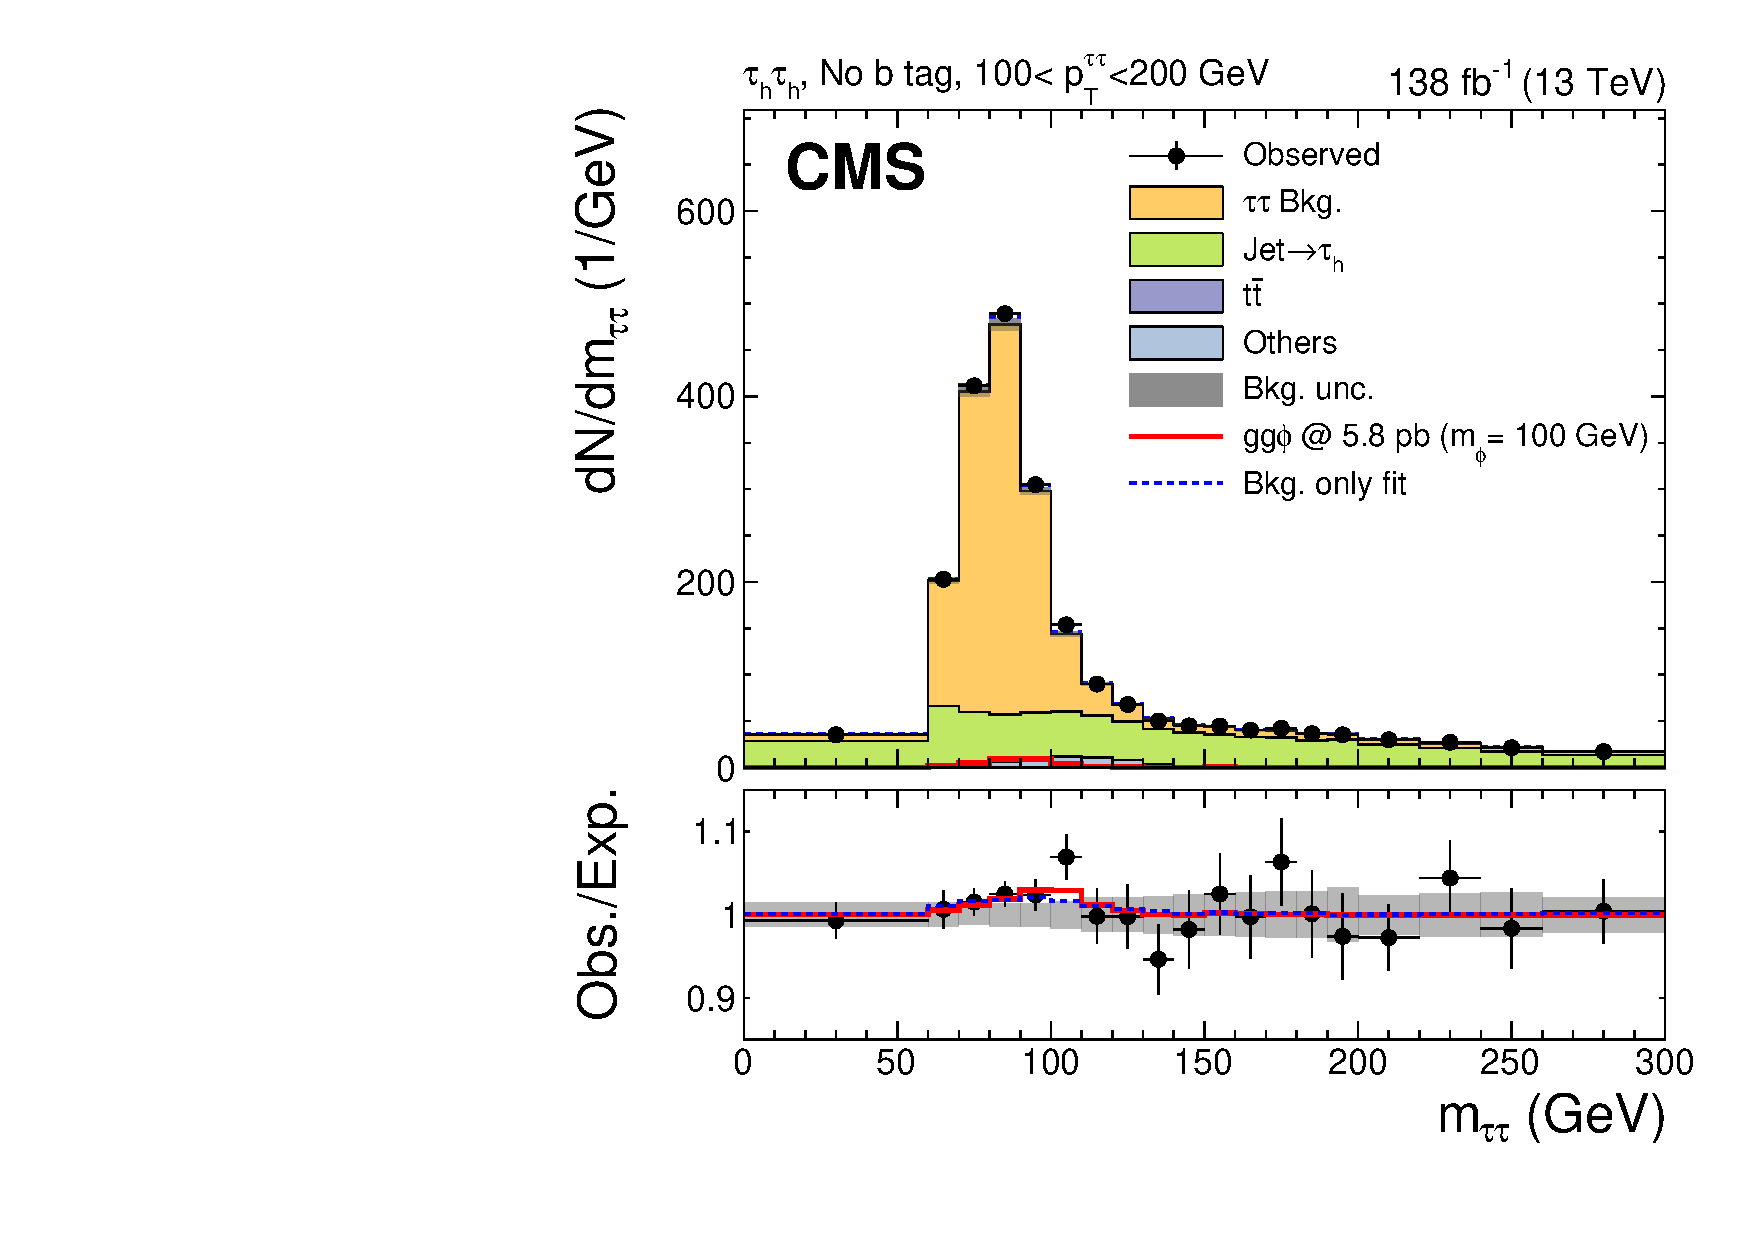
\includegraphics[width=0.4\textwidth]{Figures/postfit_lowmass_tt_nobtag_mediumpT.pdf}}
    \subfloat[]{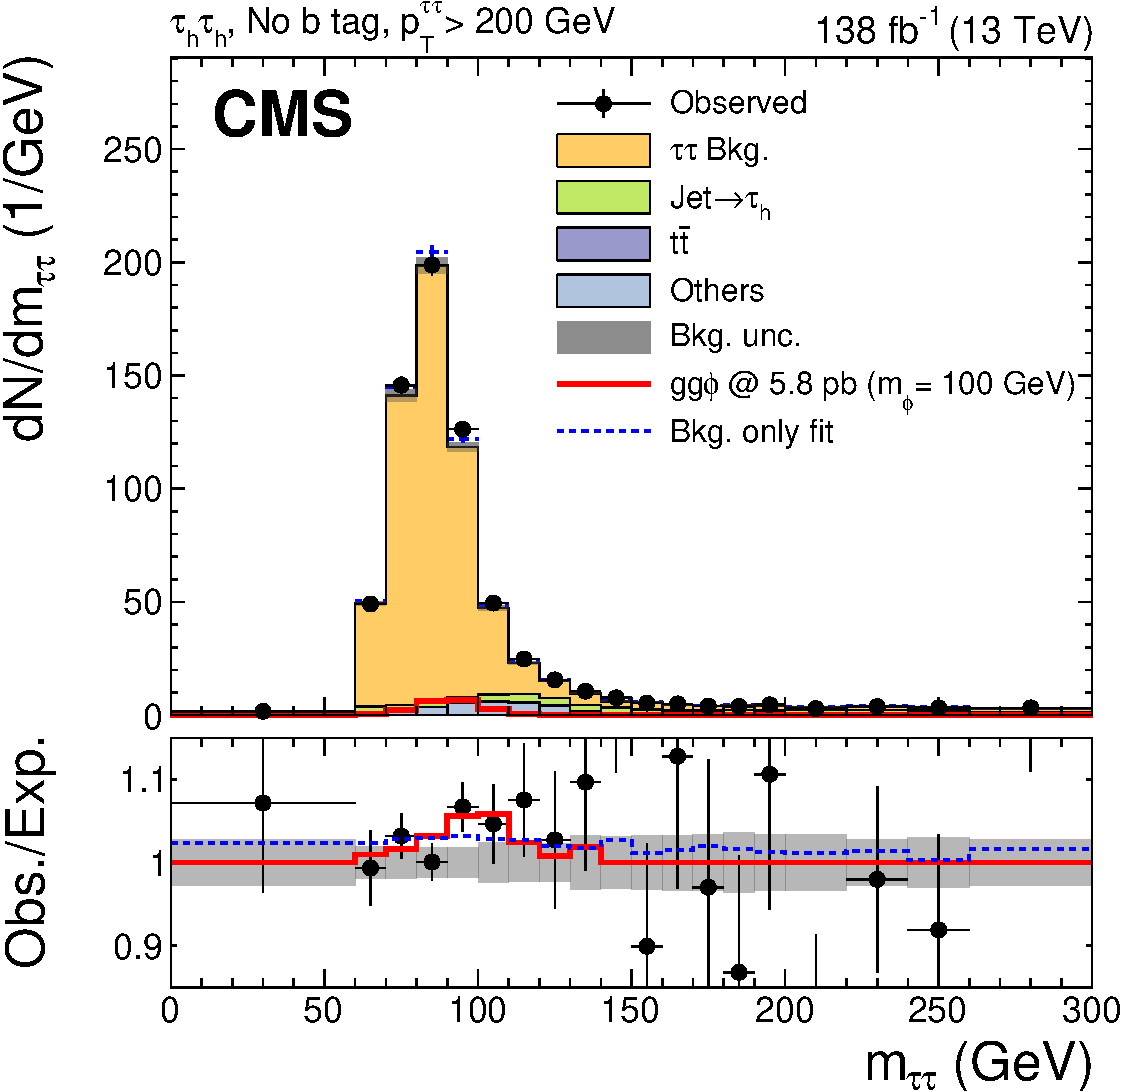
\includegraphics[width=0.4\textwidth]{Figures/postfit_lowmass_tt_nobtag_highpT-cropped.pdf}} \\
    \subfloat[]{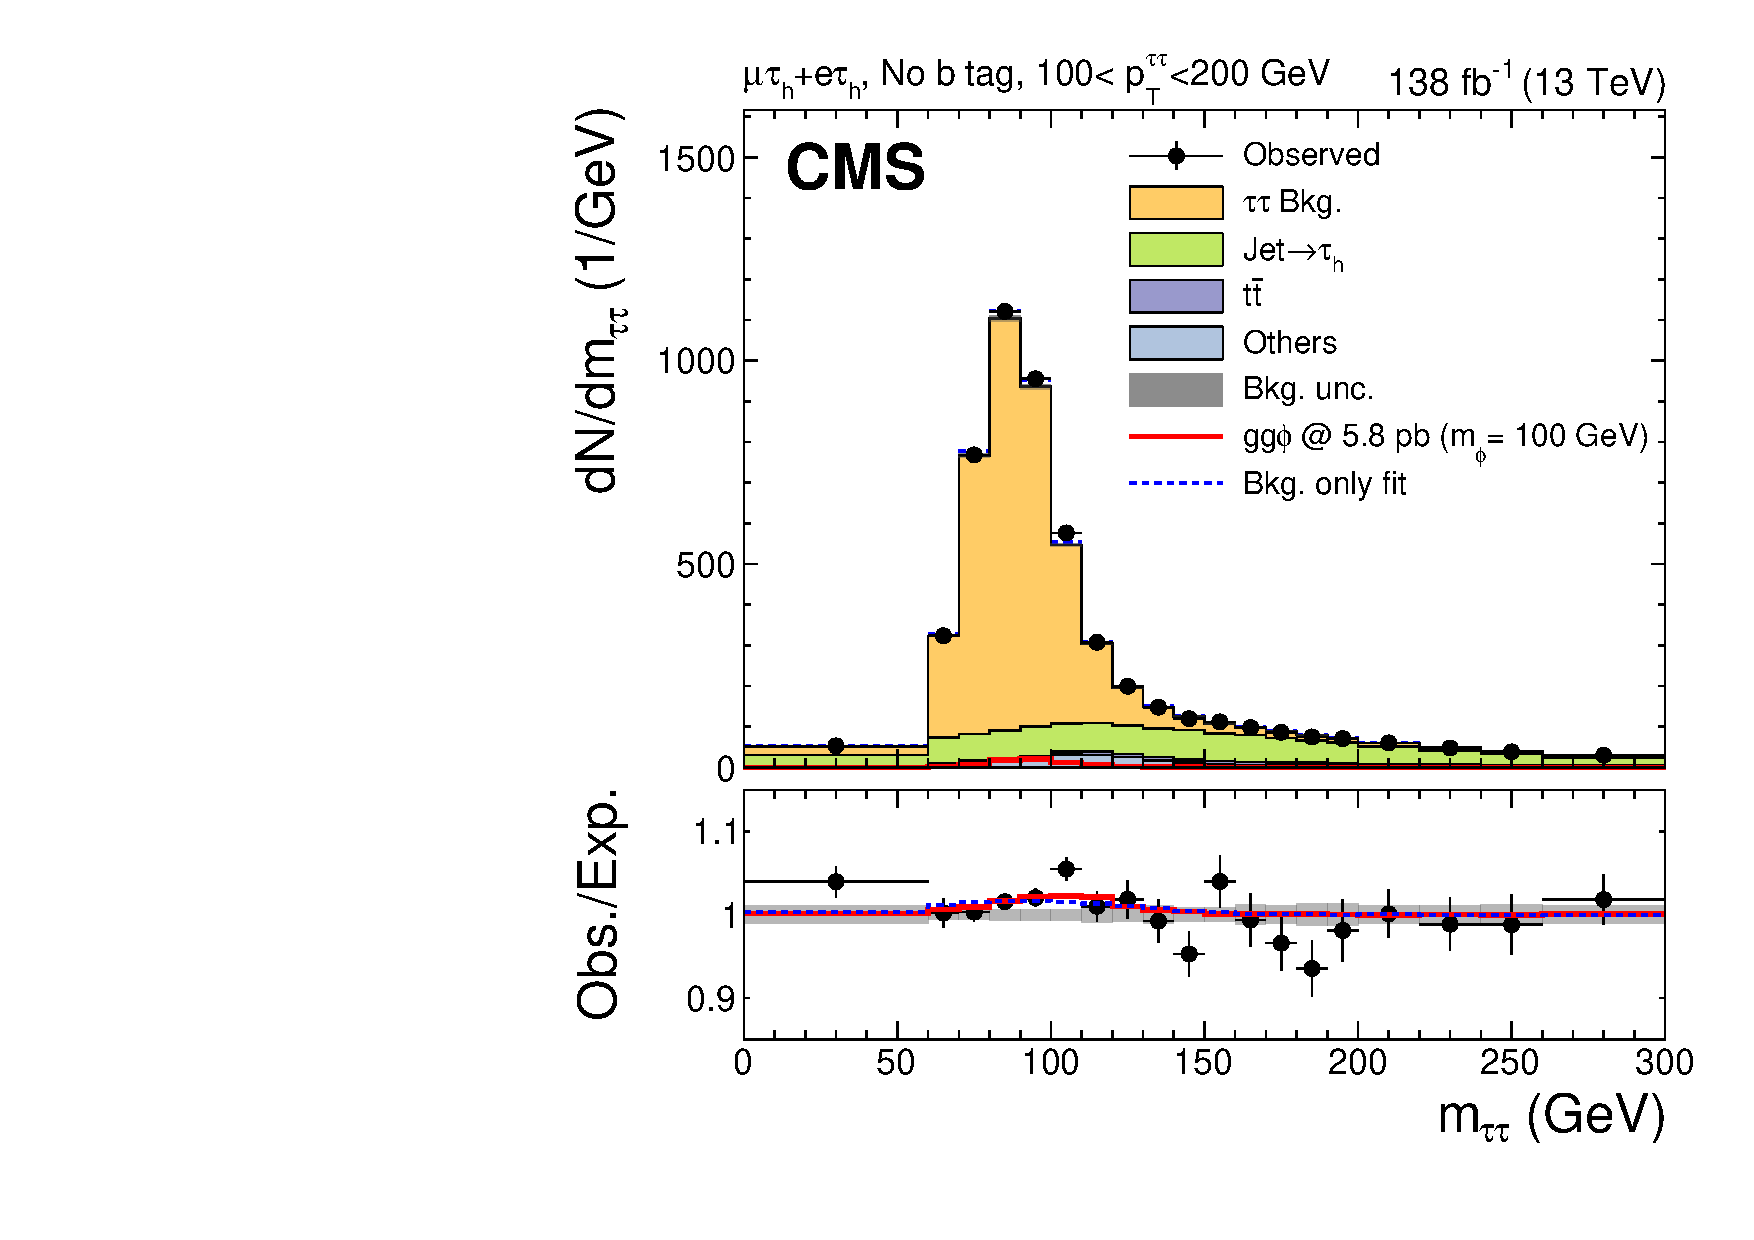
\includegraphics[width=0.4\textwidth]{Figures/postfit_lowmass_lt_nobtag_mediumpT.pdf}}
    \subfloat[]{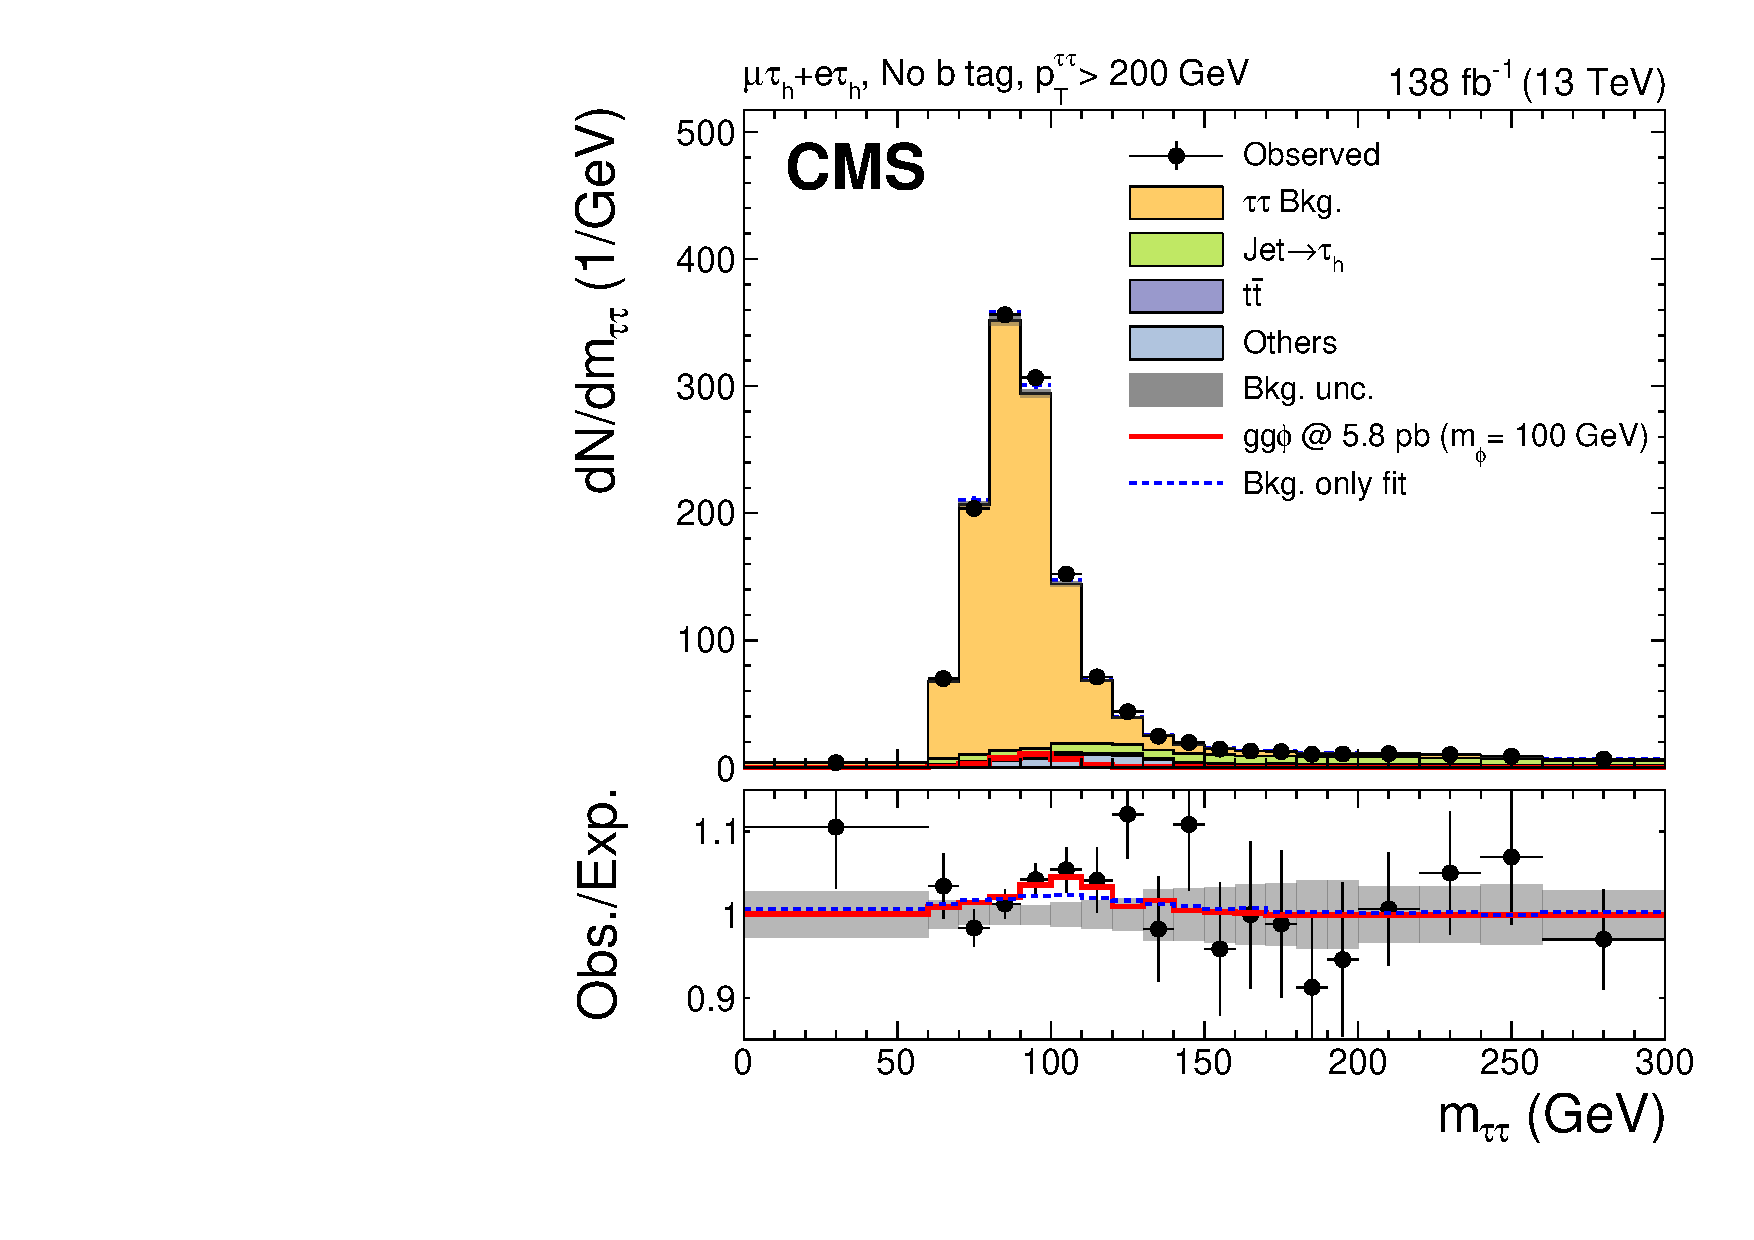
\includegraphics[width=0.4\textwidth]{Figures/postfit_lowmass_lt_nobtag_highpT.pdf}} \\
    \subfloat[]{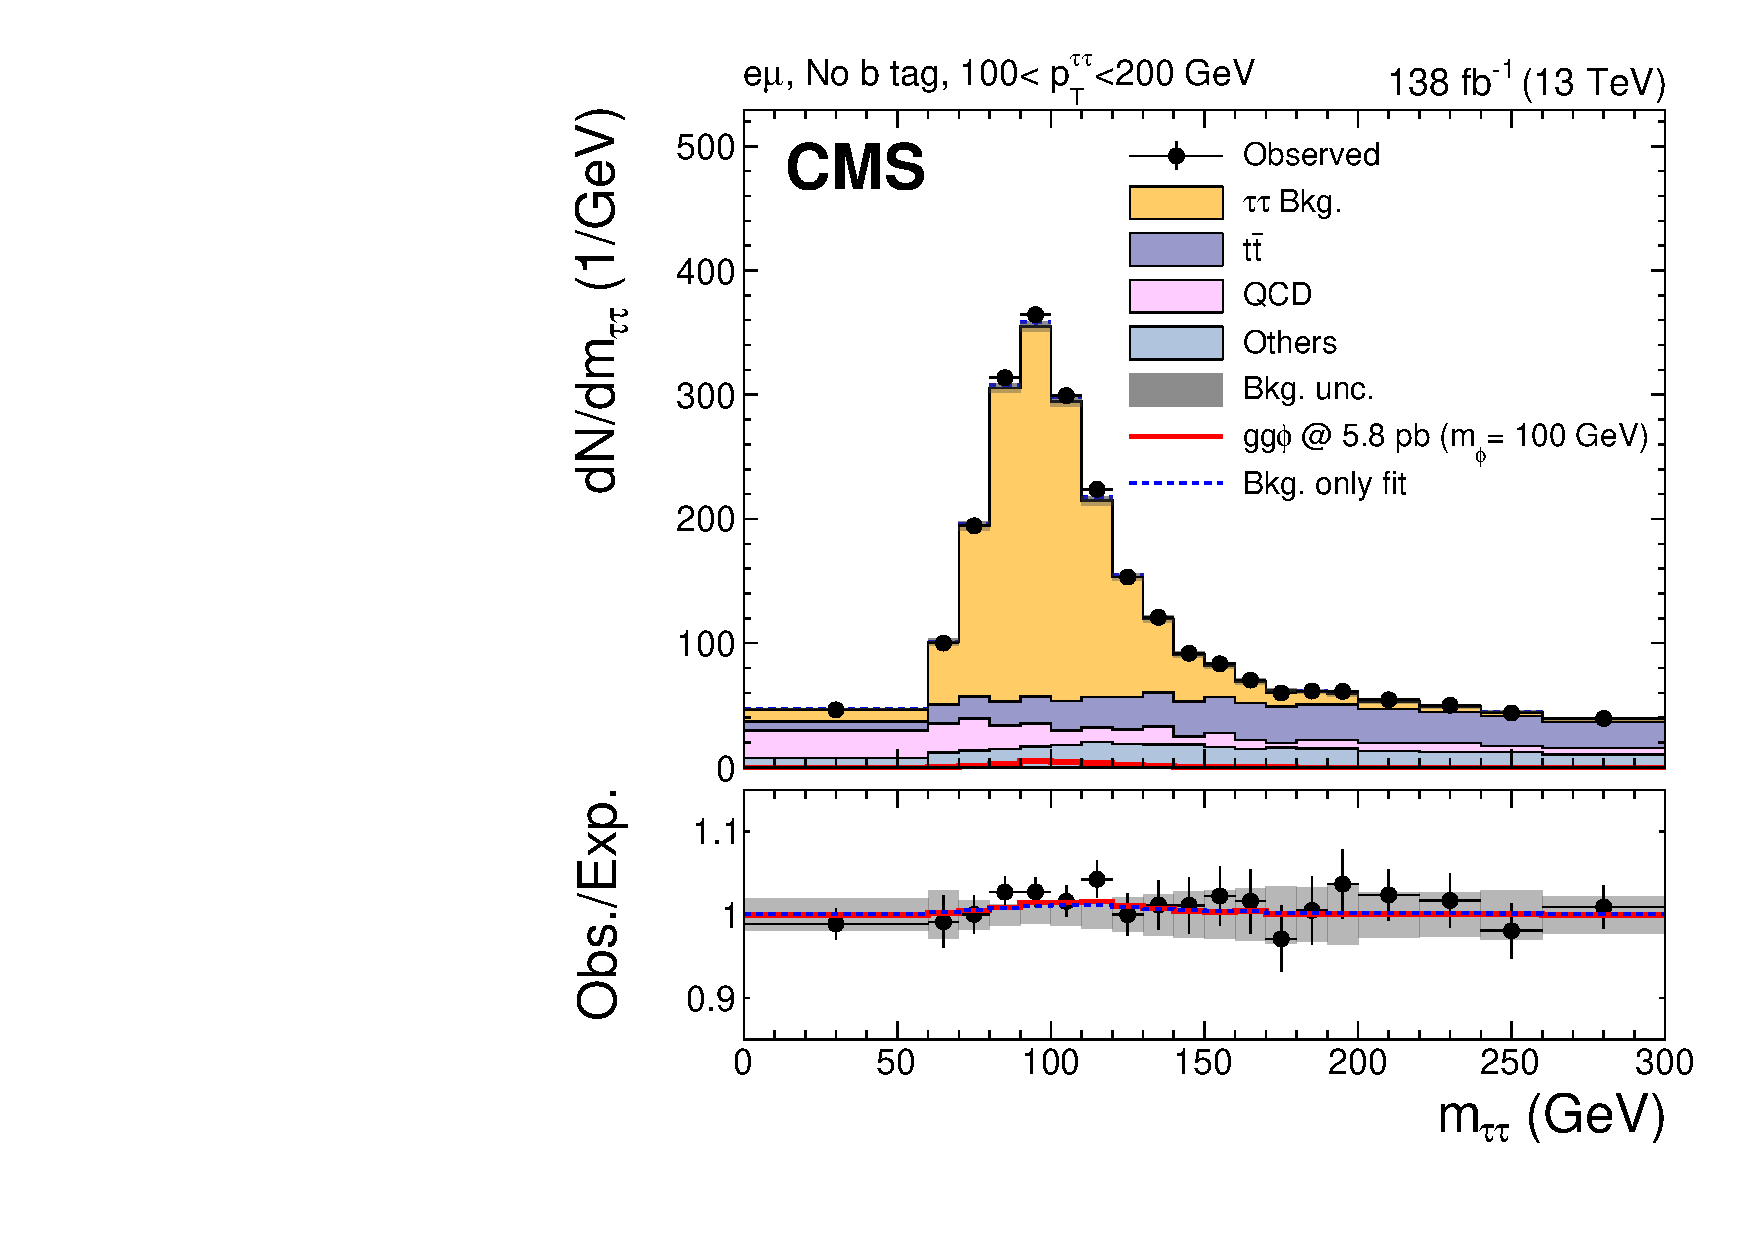
\includegraphics[width=0.4\textwidth]{Figures/postfit_lowmass_em_nobtag_mediumpT.pdf}}
    \subfloat[]{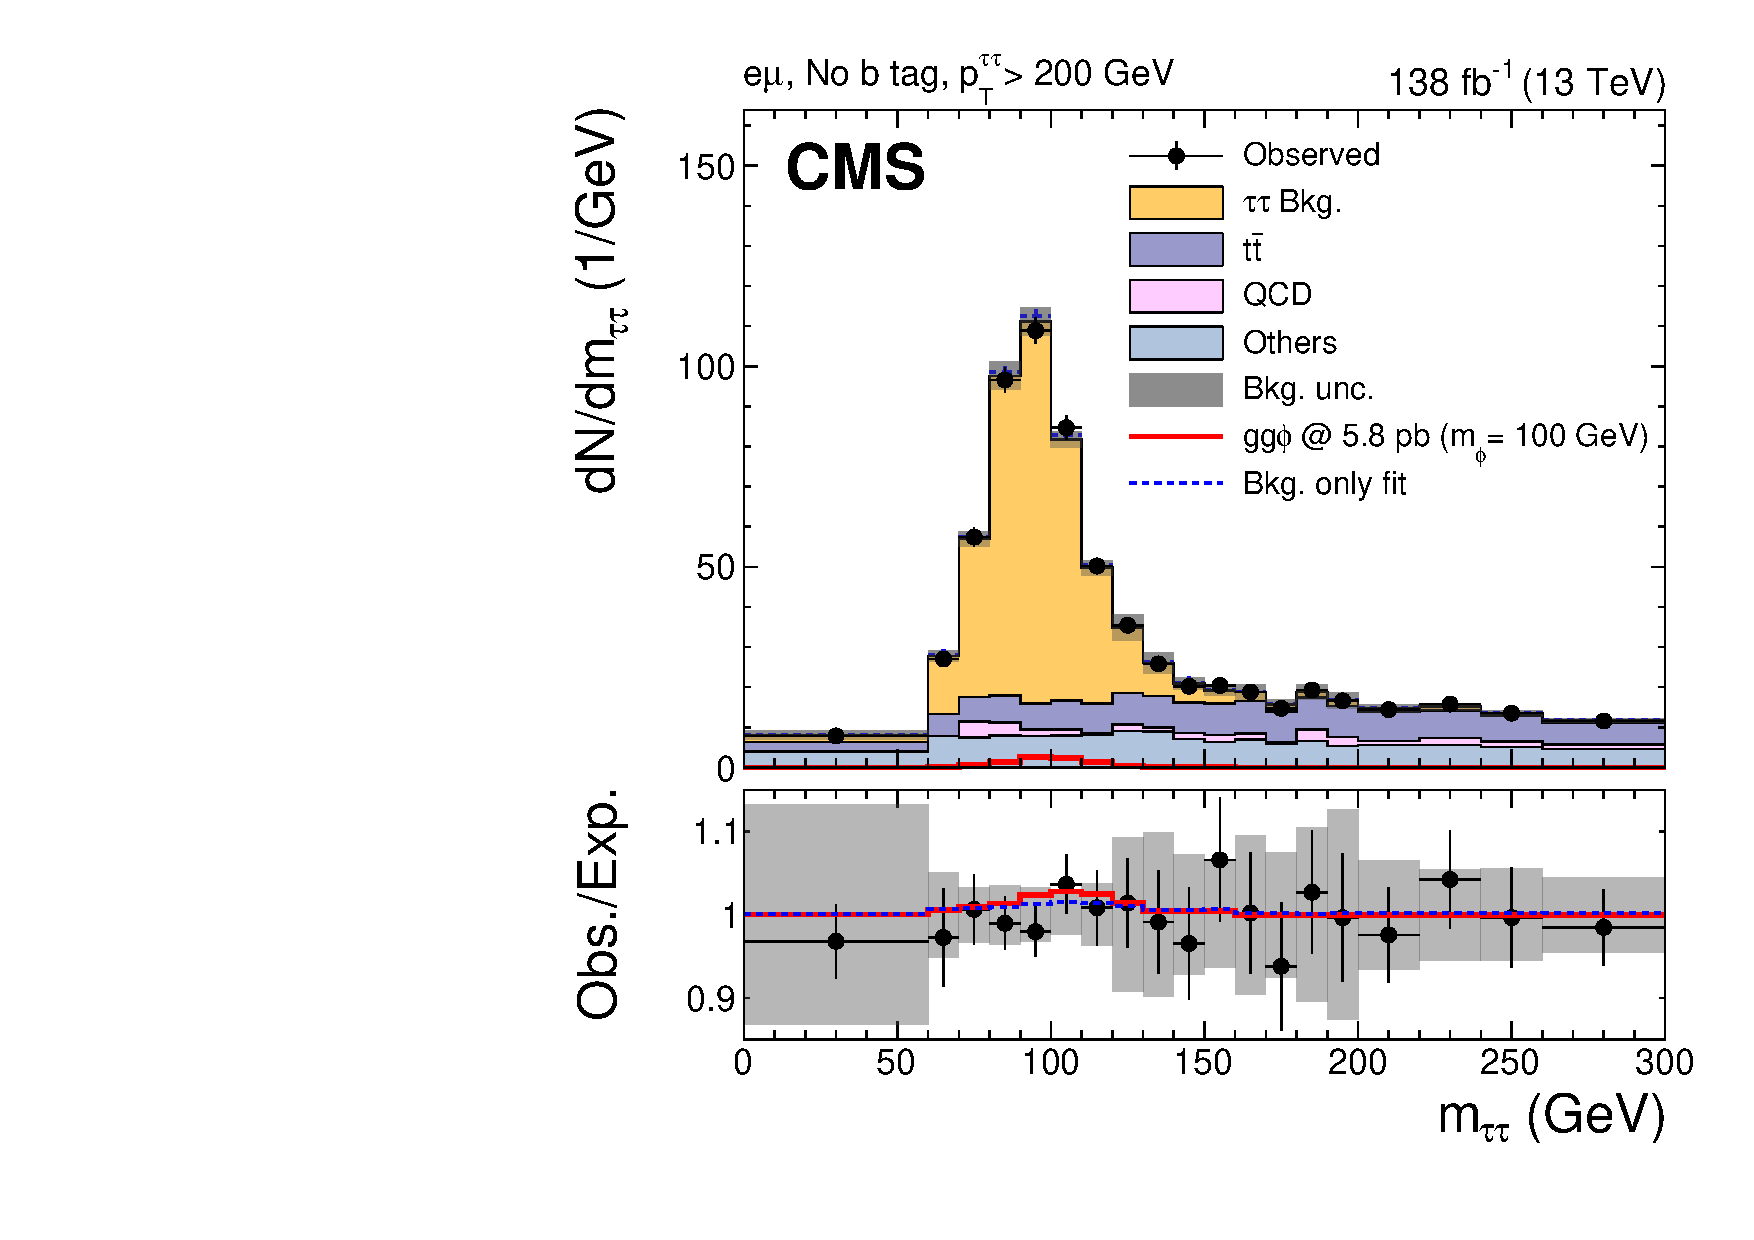
\includegraphics[width=0.4\textwidth]{Figures/postfit_lowmass_em_nobtag_highpT.pdf}}
\caption{Distributions of $m_{\tau\tau}$ in the no b tag second highest (left) and highest (right) $\pT$ category for the $\tauhtauh$ (top), the combined $\etauh$ and $\mutauh$ (middle) and the $\emu$ (bottom) channels. The solid histograms show the stacked background predictions after a signal plus background fit to the data. The best fit gluon fusion signal for $m_{\phi}$ = 100 GeV is shown by the red line. Also shown by a blue dashed line on the bottom pad is the ratio of the background predictions for the background only fit to the signal plus background fit }
\label{fig:low_mass_postfit}
\end{figure}

\begin{figure}[!hbtp]
\centering
    \subfloat[]{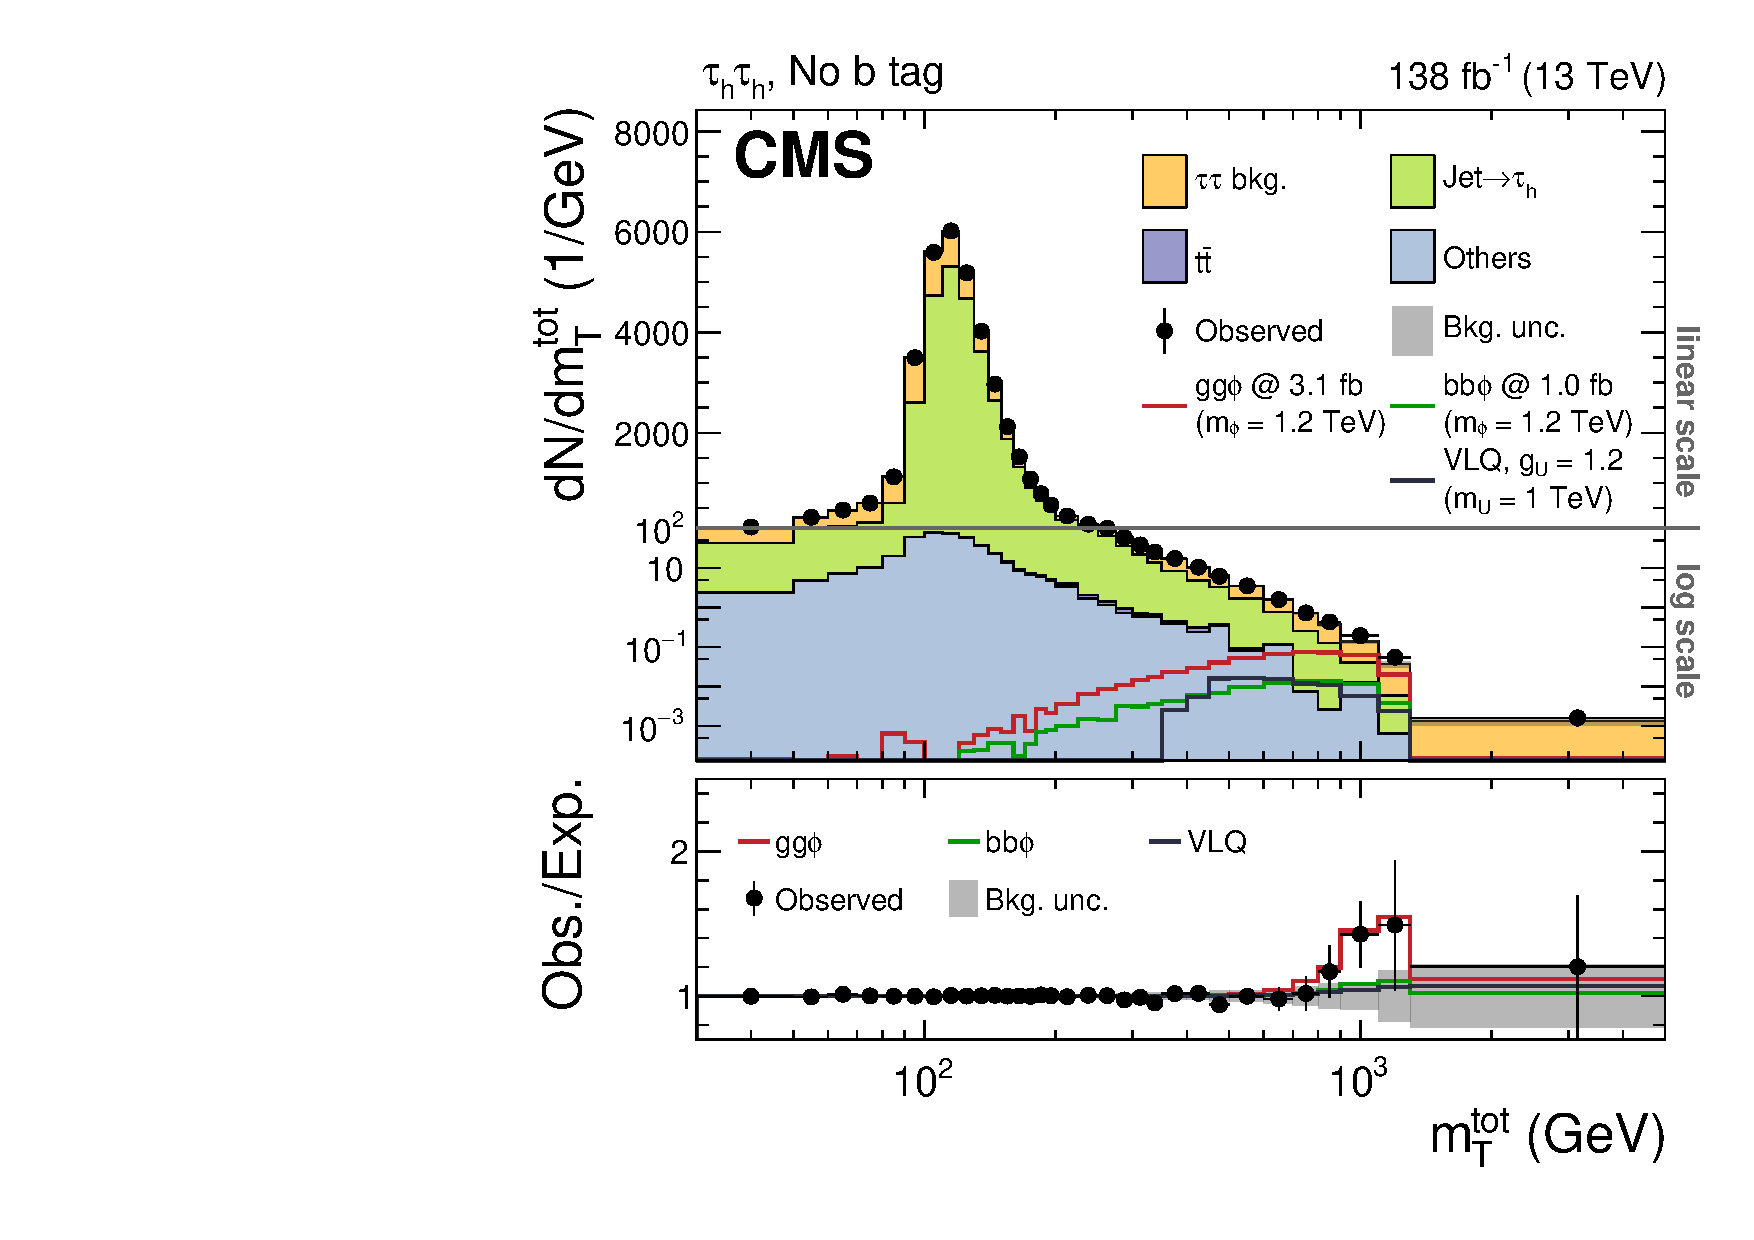
\includegraphics[width=0.42\textwidth]{Figures/postfit_highmass_tt_nobtag.pdf}}
    \subfloat[]{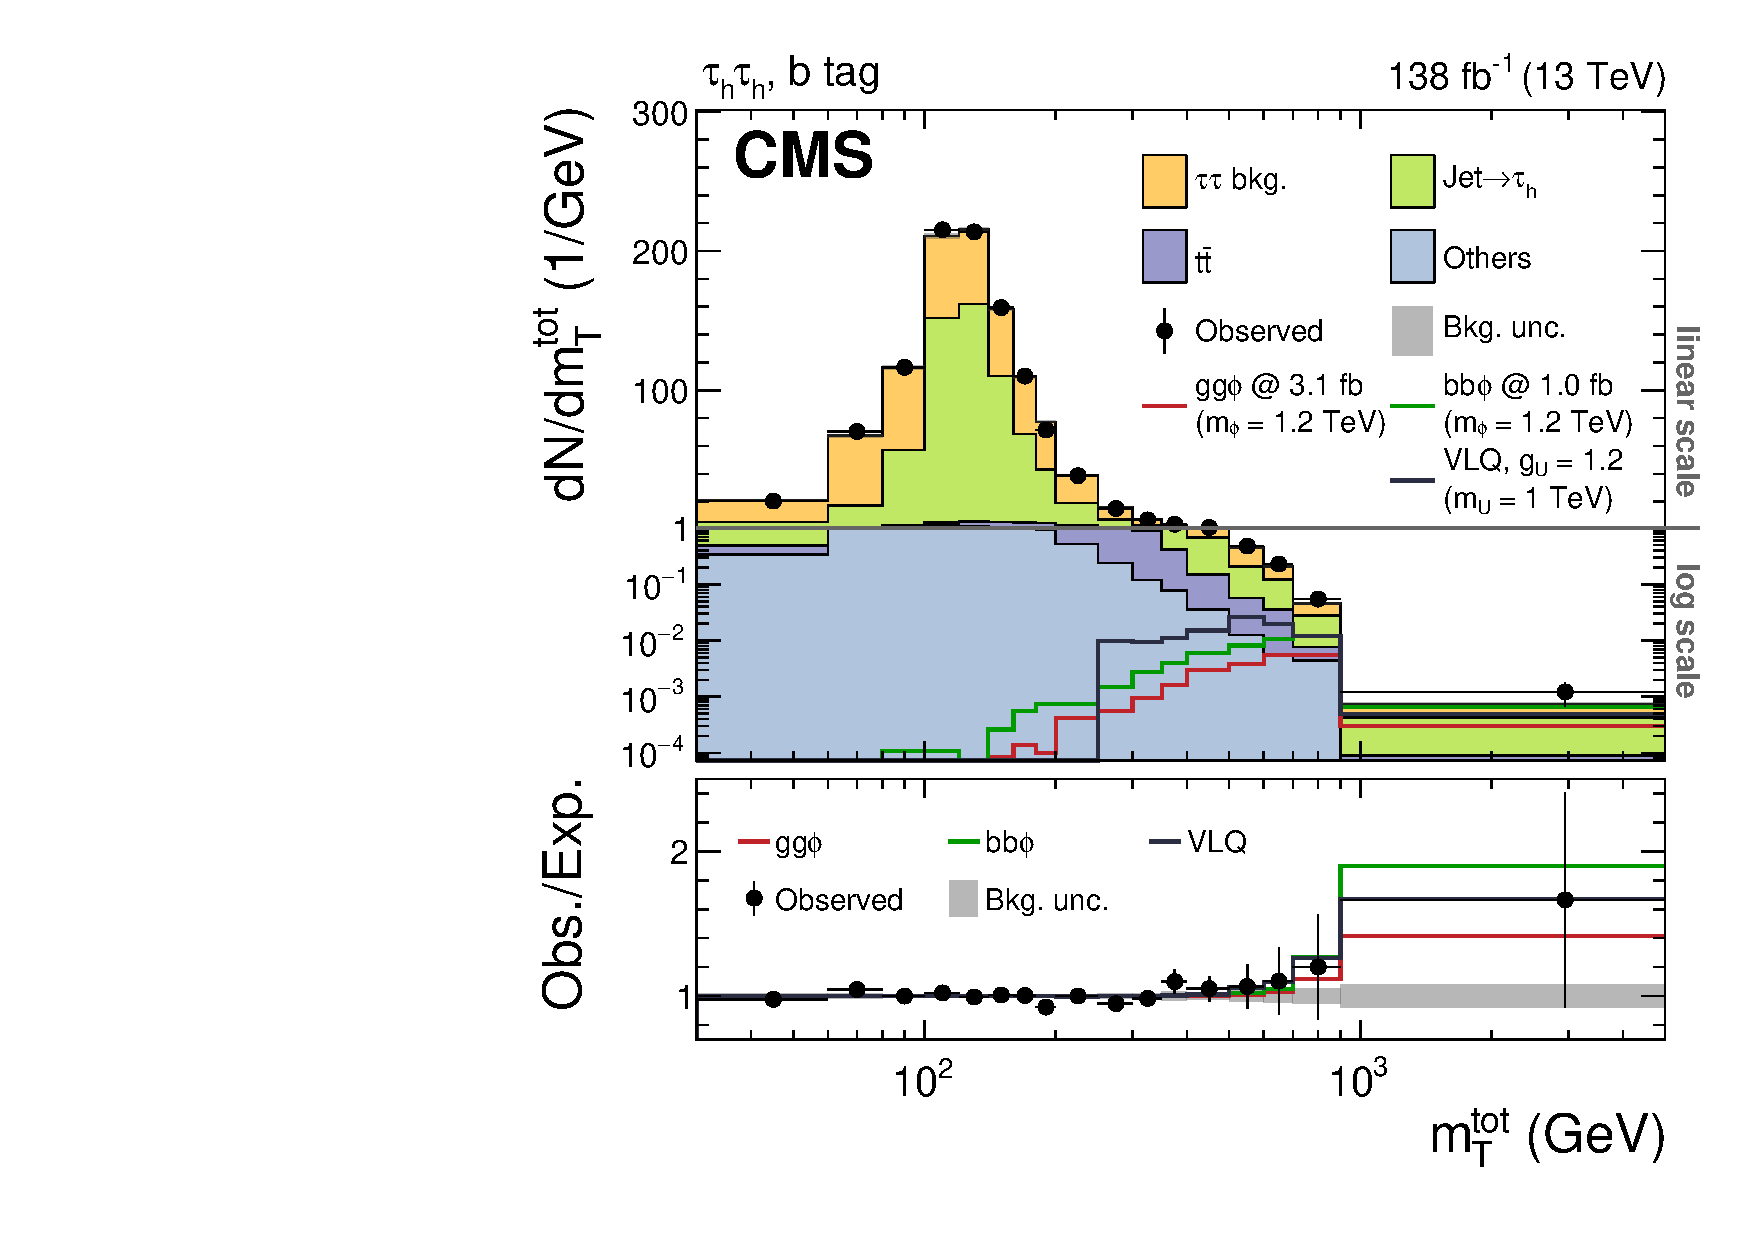
\includegraphics[width=0.42\textwidth]{Figures/postfit_highmass_tt_btag.pdf}} \\
    \subfloat[]{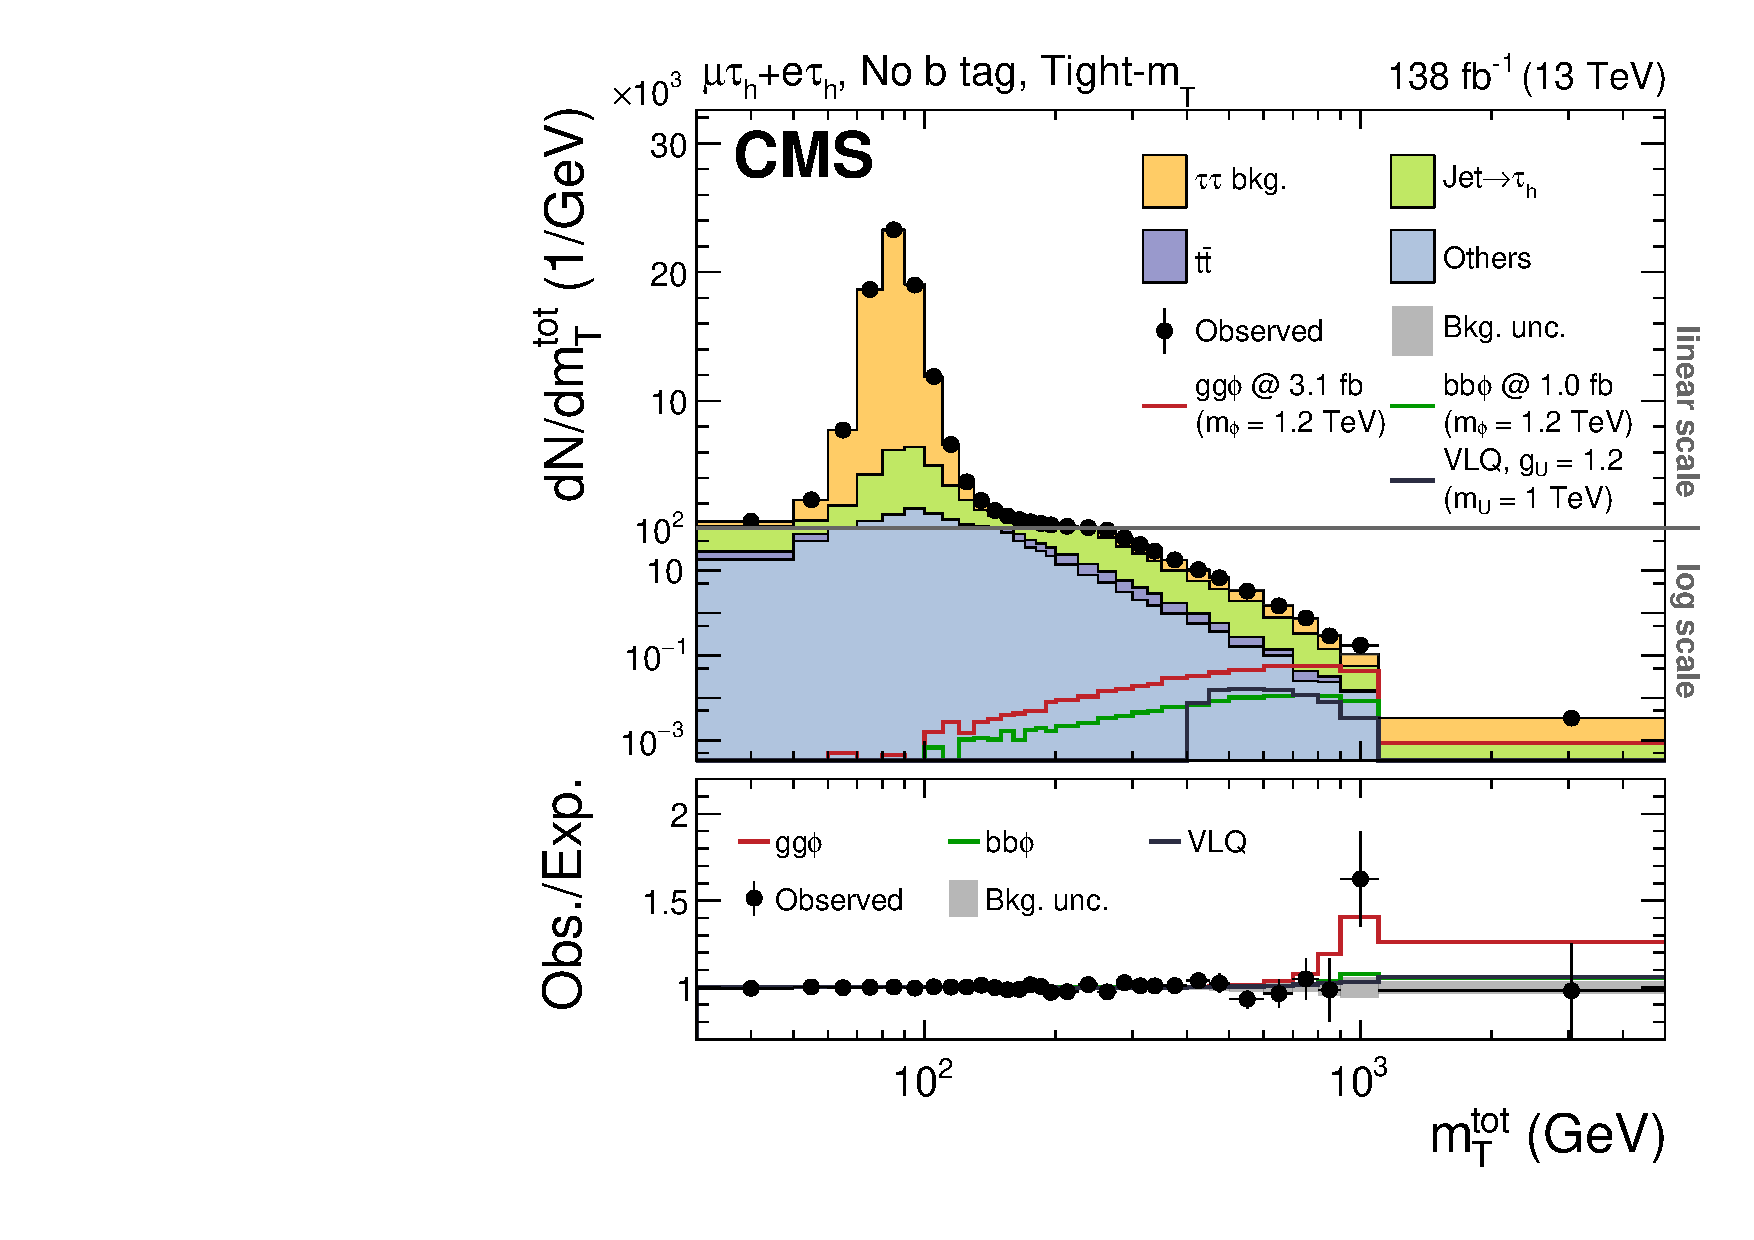
\includegraphics[width=0.42\textwidth]{Figures/postfit_highmass_lt_nobtag_tightmT.pdf}}
    \subfloat[]{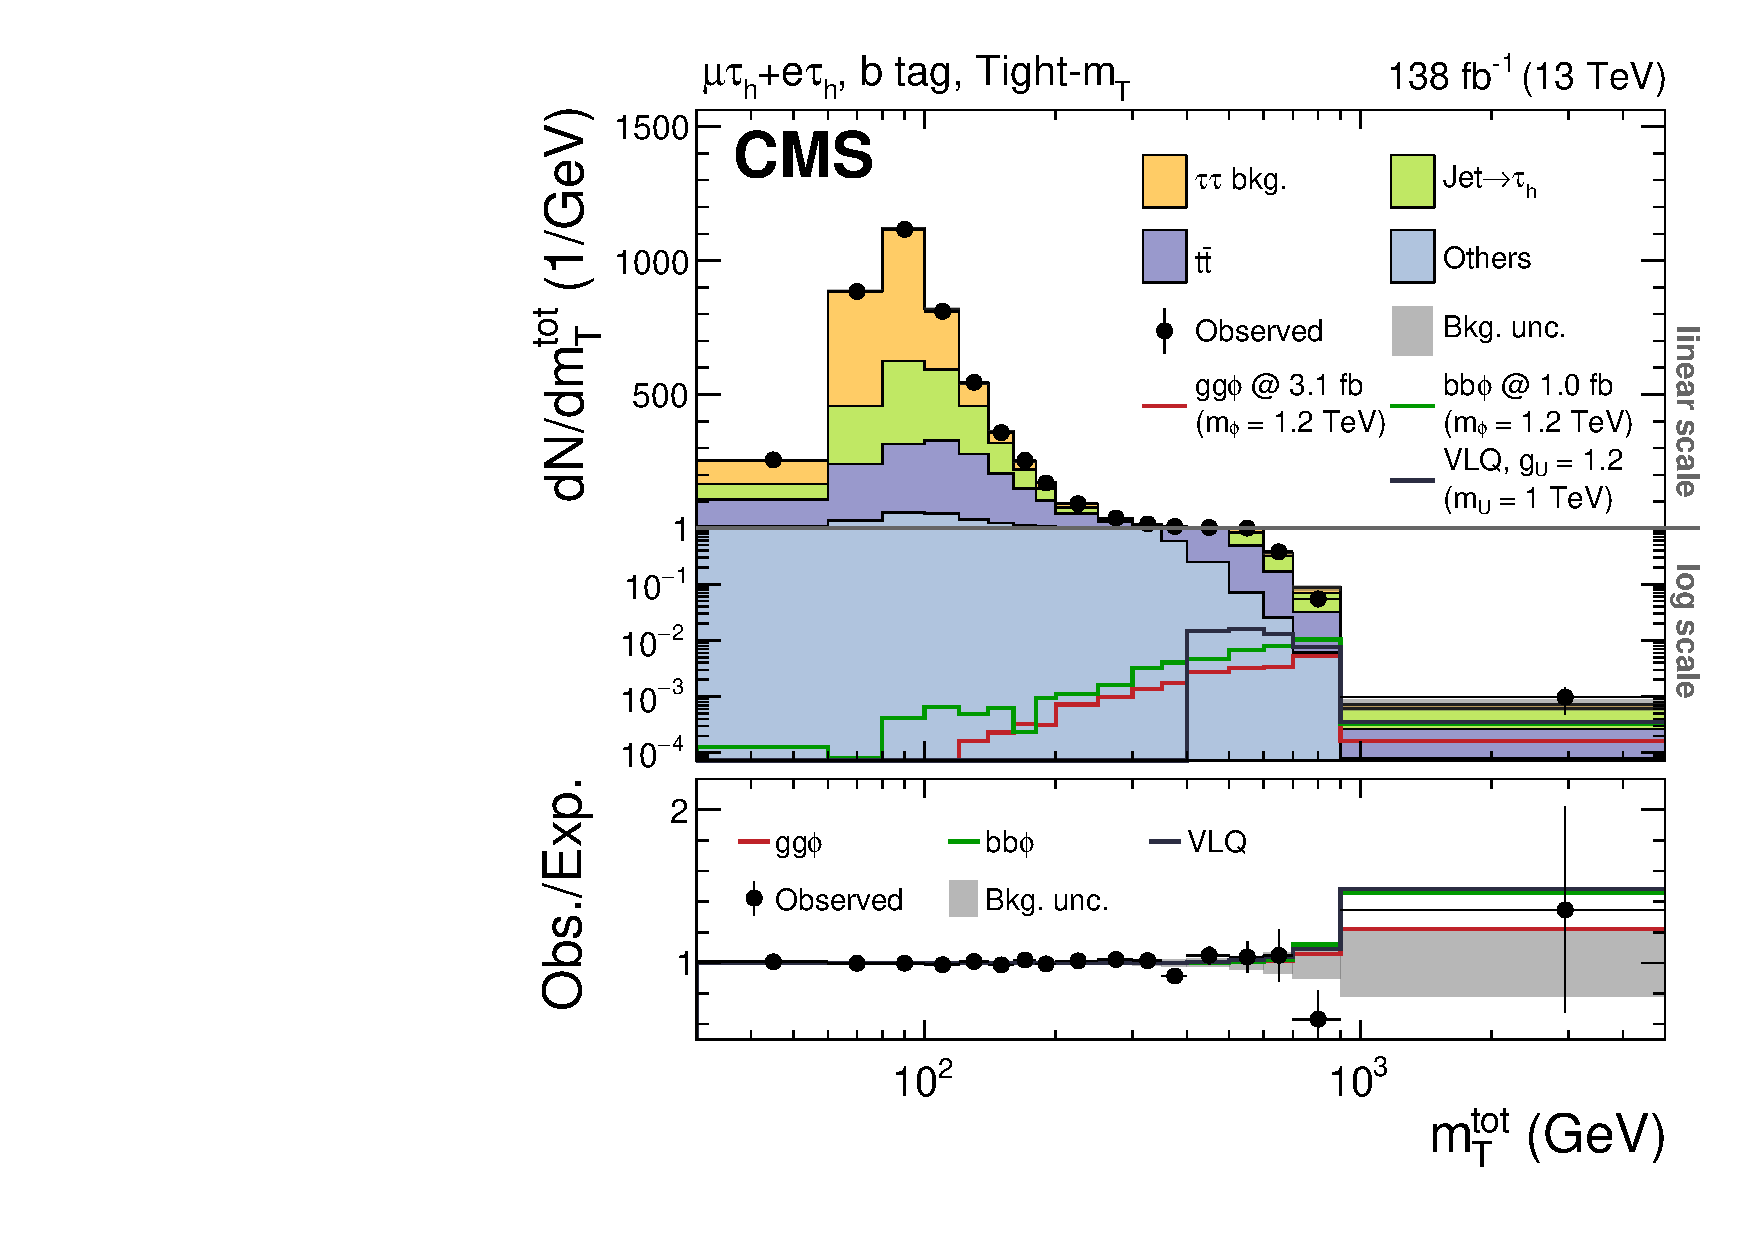
\includegraphics[width=0.42\textwidth]{Figures/postfit_highmass_lt_btag_tightmT.pdf}} \\
    \subfloat[]{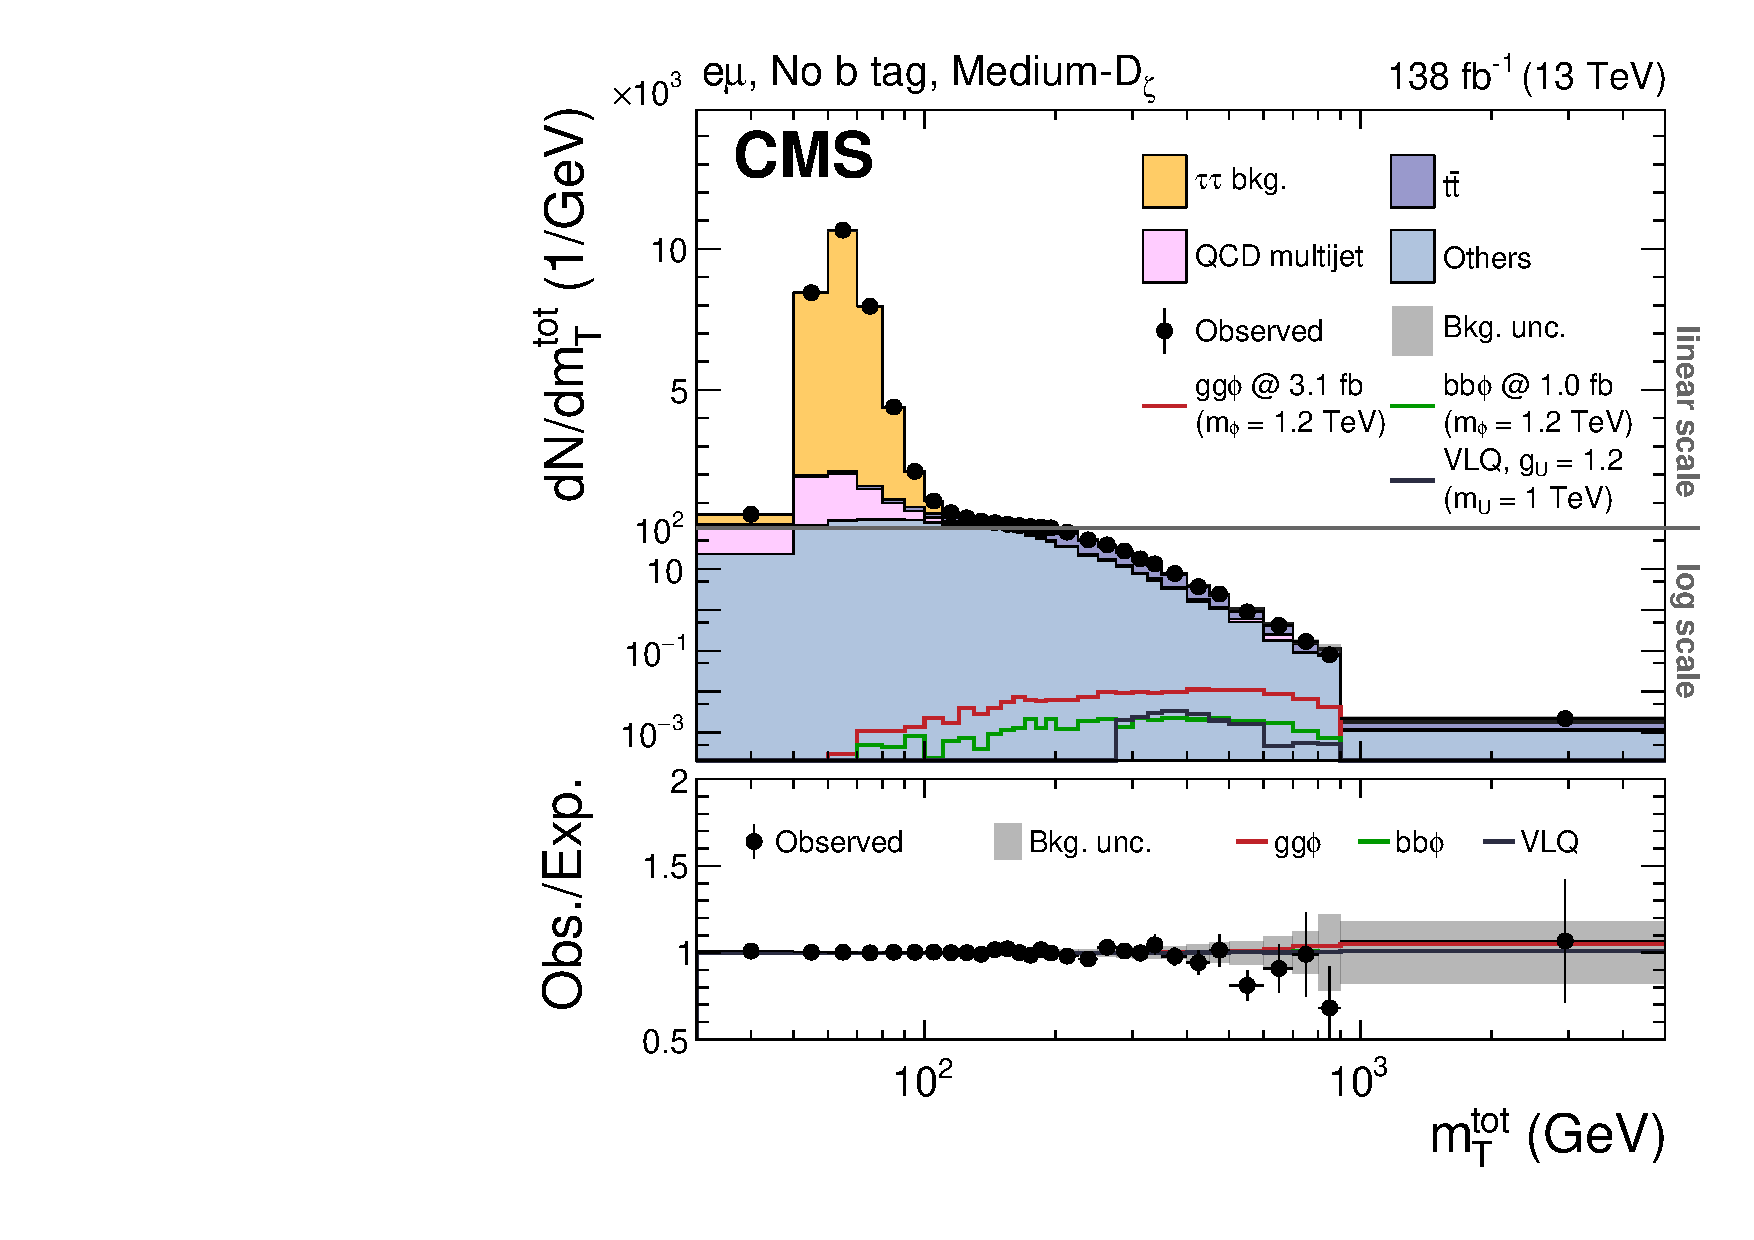
\includegraphics[width=0.42\textwidth]{Figures/postfit_highmass_em_nobtag_mediumdzeta.pdf}}
    \subfloat[]{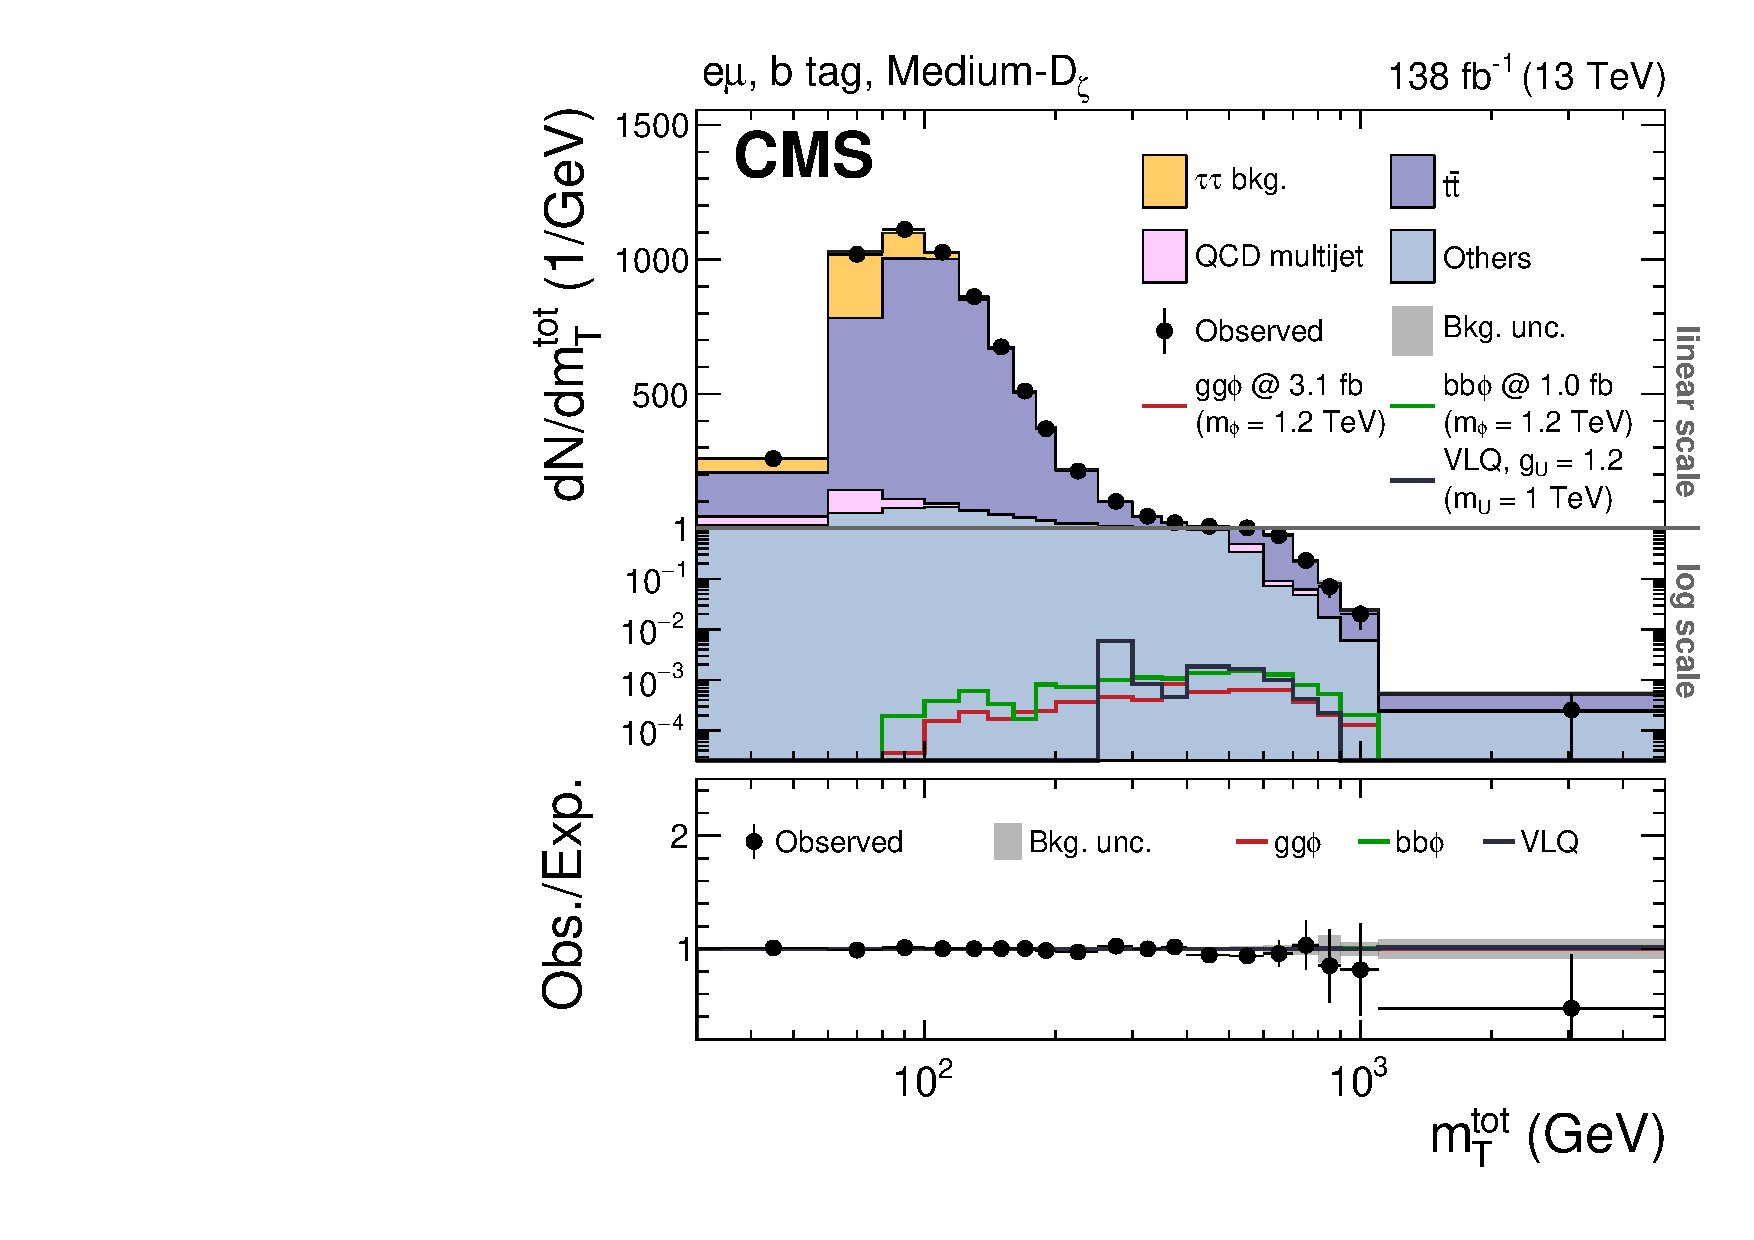
\includegraphics[width=0.42\textwidth]{Figures/postfit_highmass_em_btag_mediumdzeta.pdf}}
\caption{Distributions of $m_{T}^\text{tot}$ in the $\tauhtauh$ no b tag (a) and b tag (b) categories, the combined $\etauh$ and $\mutauh$ no b tag (c) and b tag (d) Tight-$m_{T}$ categories and the $\emu$ no b tag (e) and b tag (f) Medium-$D_{\zeta}$ categories. The solid histograms show the stacked background predictions after a background only fit to the data. The best fit gluon fusion signal for $m_{\phi}$ = 1.2 TeV is shown by the red line, b associated production and $U_{1}$ signals are also shown for illustrative purposes.}
\label{fig:high_mass_postfit}
\end{figure}

\newpage
\section{Model Independent Results}

\subsection{Limits}

95\% CL limits are set on the assumption of absence of a signal for the search for a gg$\phi$ or bb$\phi$ resonance and shown in Figure~\ref{fig:model_independent_limits}.
In each case, the other process is allowed to float freely in the fit.
The excesses observed in the postfit distributions act to weaken the observed limit compared to the expected limit at 100 GeV and 1.2 TeV, as more data was observed than expected.
For gg$\phi$ production the expected limits flatten under 100 GeV, due to difficulty of separating signal from the Z boson at this mass.
Both sets of limits vary from $\mathcal{O}(10\text{ pb})$ at 60 GeV to $0.3$ fb at 3.5 TeV.

\begin{figure}[!hbtp]
\centering
    \subfloat[]{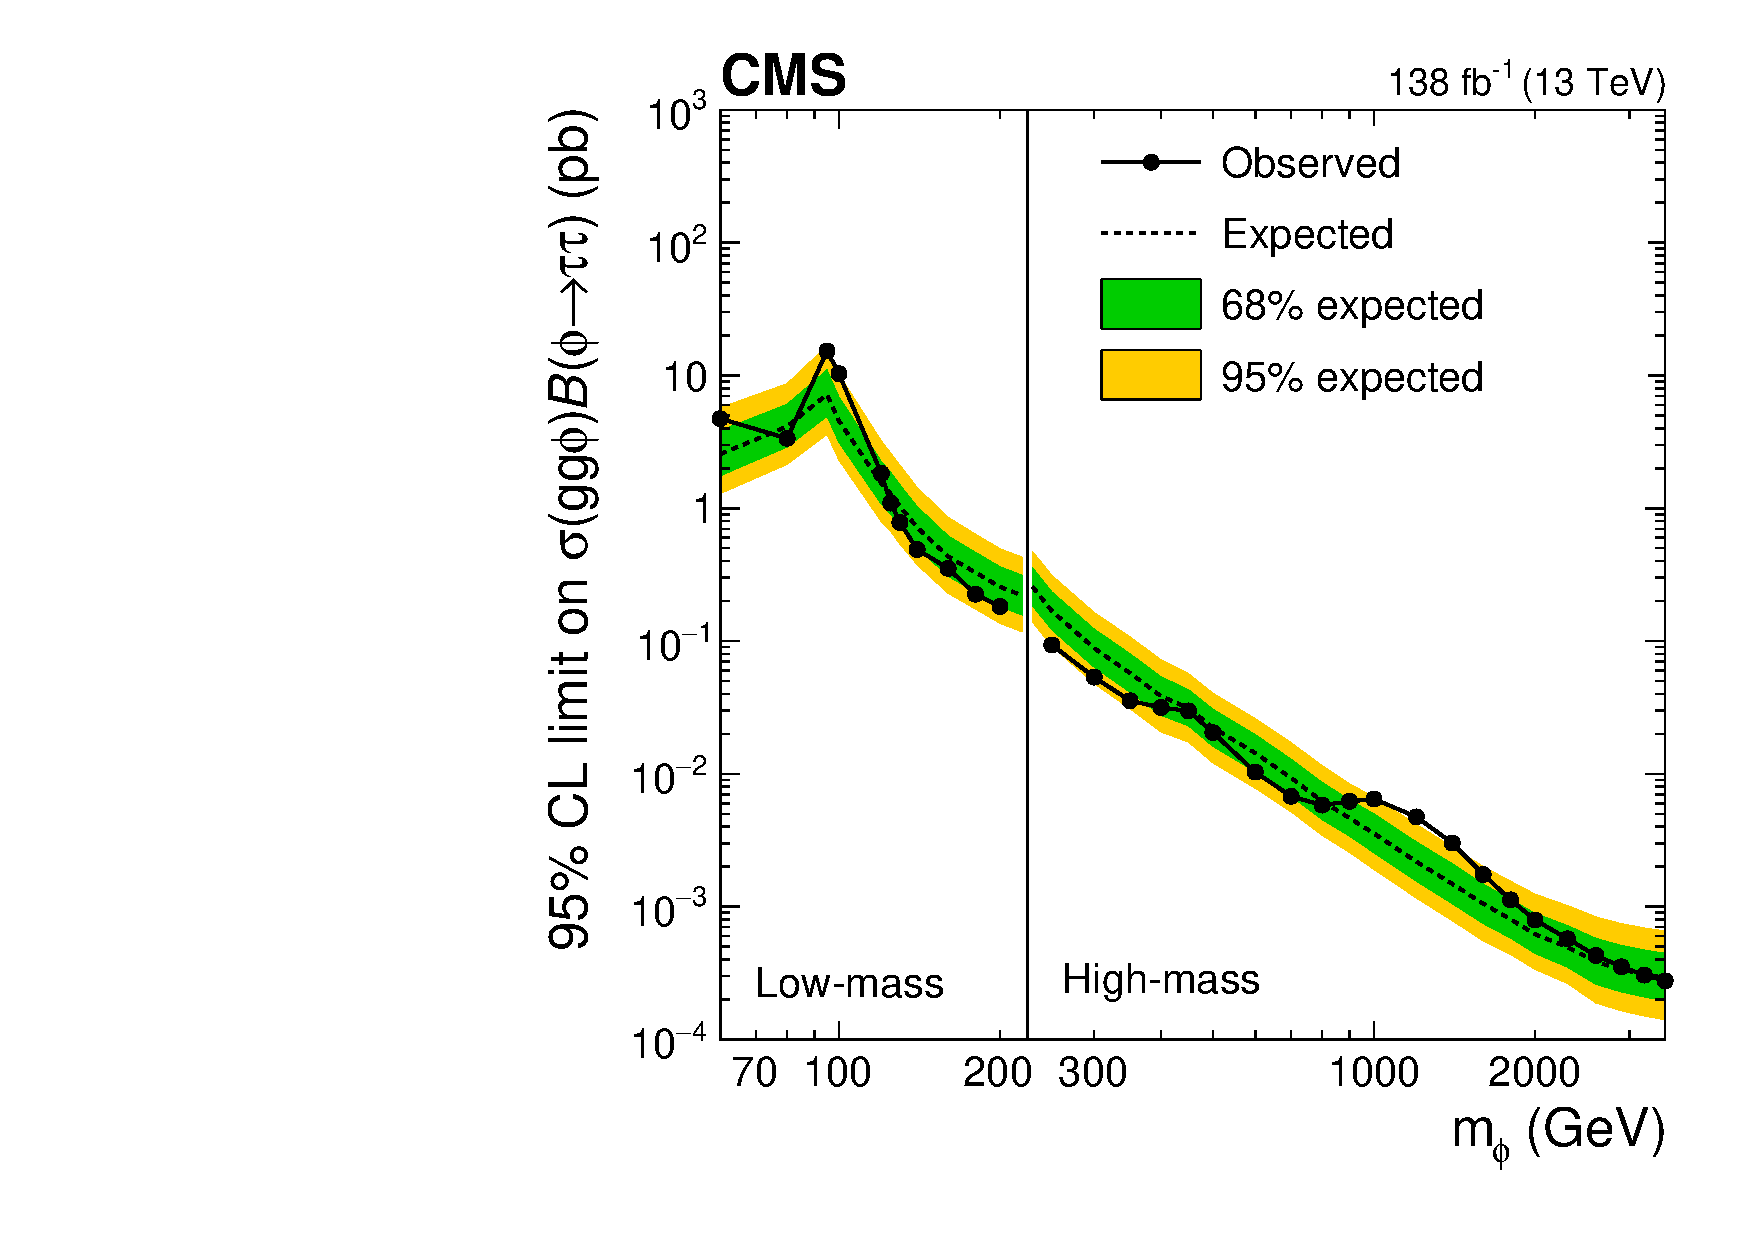
\includegraphics[width=0.5\textwidth]{Figures/model_independent_limit_ggH.pdf}}
    \subfloat[]{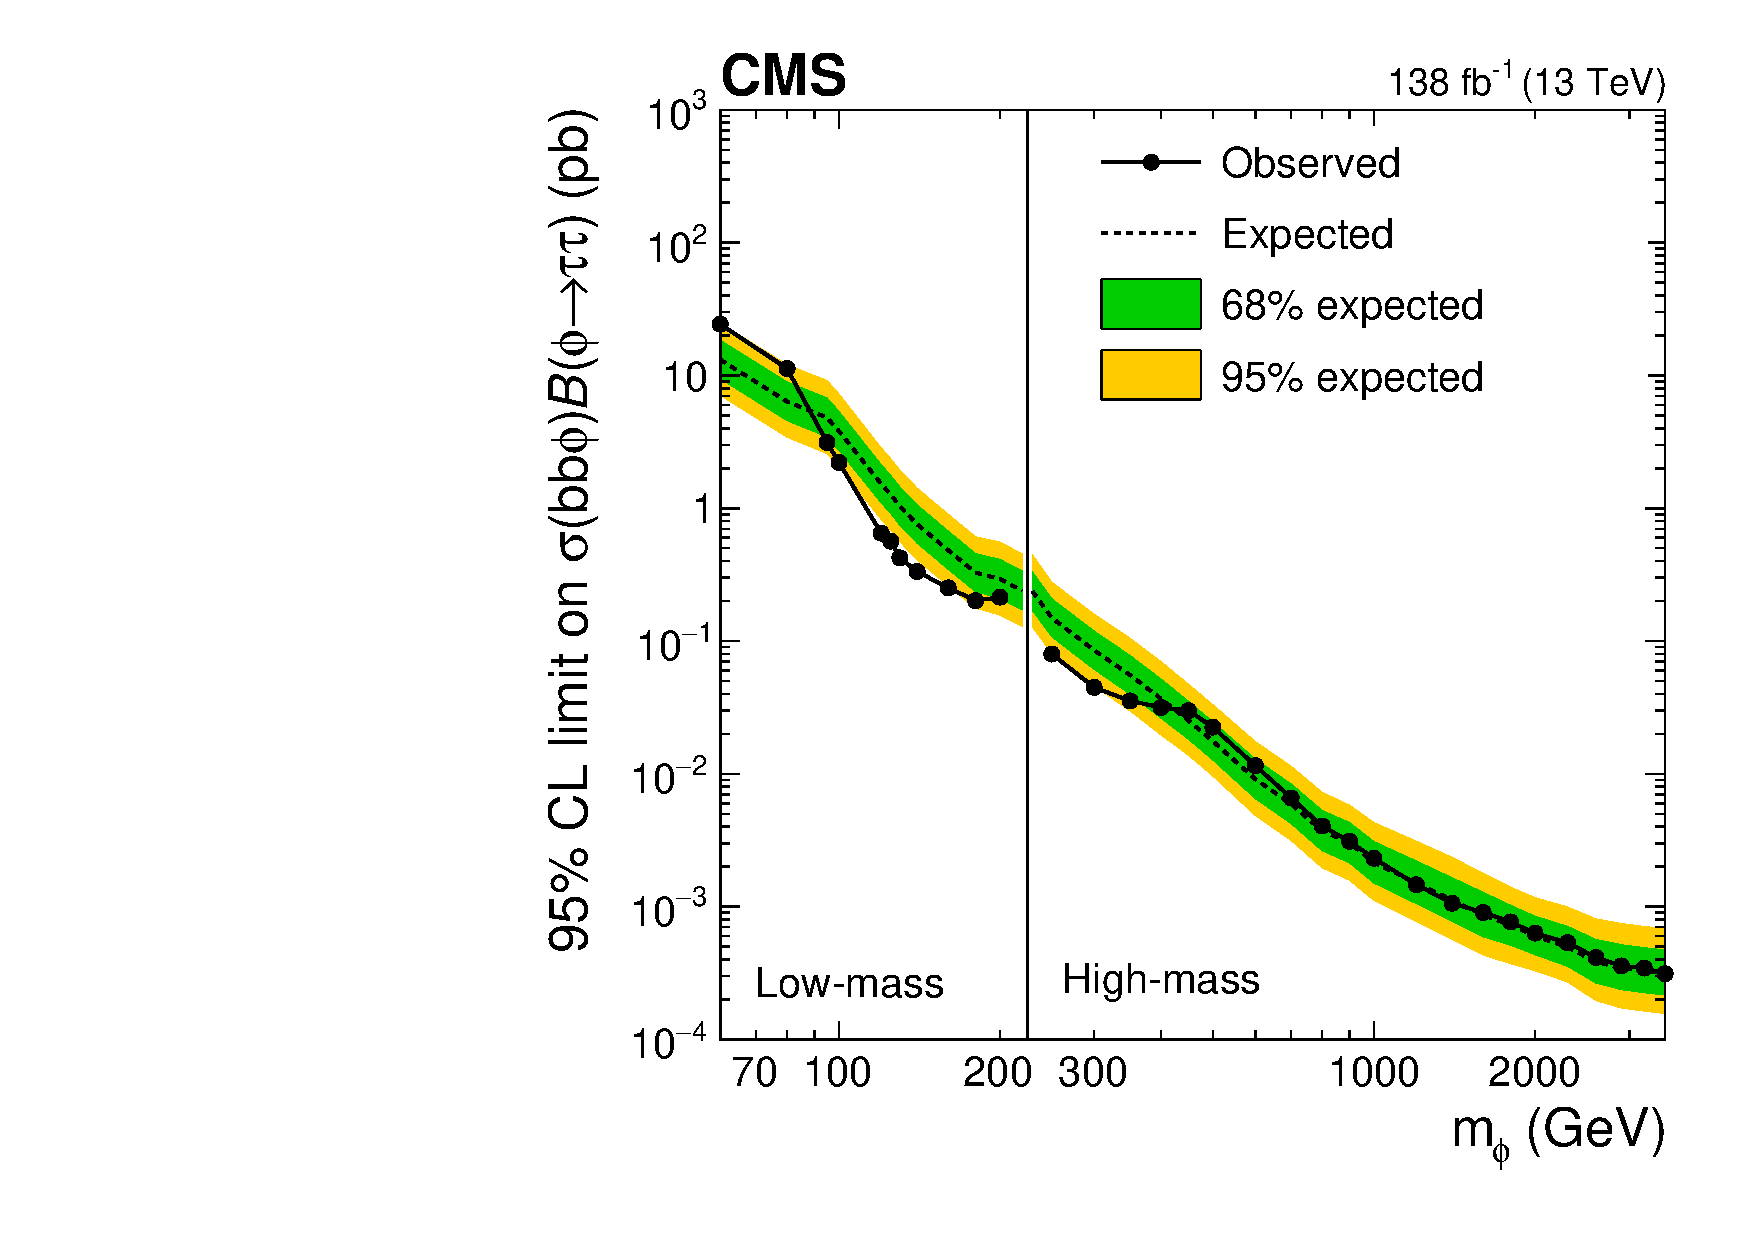
\includegraphics[width=0.5\textwidth]{Figures/model_independent_limit_bbH.pdf}}
\caption{Expected (dashed line) and observed (solid line and dots) 95\% CL upper limits on the product of the cross sections and branching fraction for the decay into $\tau$ leptons for (a) gg$\phi$ and (b) bb$\phi$ production in a mass range of 60 $\leq m_{\phi} \leq$ 3500 GeV.  The dark green and bright yellow bands indicate the central 68\% and 95\% intervals for the expected exclusion limit.}
\label{fig:model_independent_limits}
\end{figure}

95\% expected limits are drawn on the fit to each di-tau decay channel individually and are shown in Figure~\ref{fig:model_independent_limits_by_channel}.
This gives a measure of the sensitivity of each channel.
In the high mass optimisation categories, the combined limit is heavily dominated by the $\tauhtauh$ channel.
This is mostly driven purely by branching fraction, as all channels in this mass range have similar signal separation ability.
In the high mass optimisation categories,  the combined limit is more a contribution of all channels. 
In the $\tauhtauh$ channel in this region, the QCD multijet background is the largest fraction of any non $Z\rightarrow\tau\tau$ backgrounds in all channels and so the limit for this channel is weakened and the other channels contribute to the combined limit more.
The high DoubleTau trigger $\pT$ thresholds (chosen because of the QCD multijet background) also lowers the signal acceptance in the $\tauhtauh$ channel.

\begin{figure}[!hbtp]
\centering
    \subfloat[]{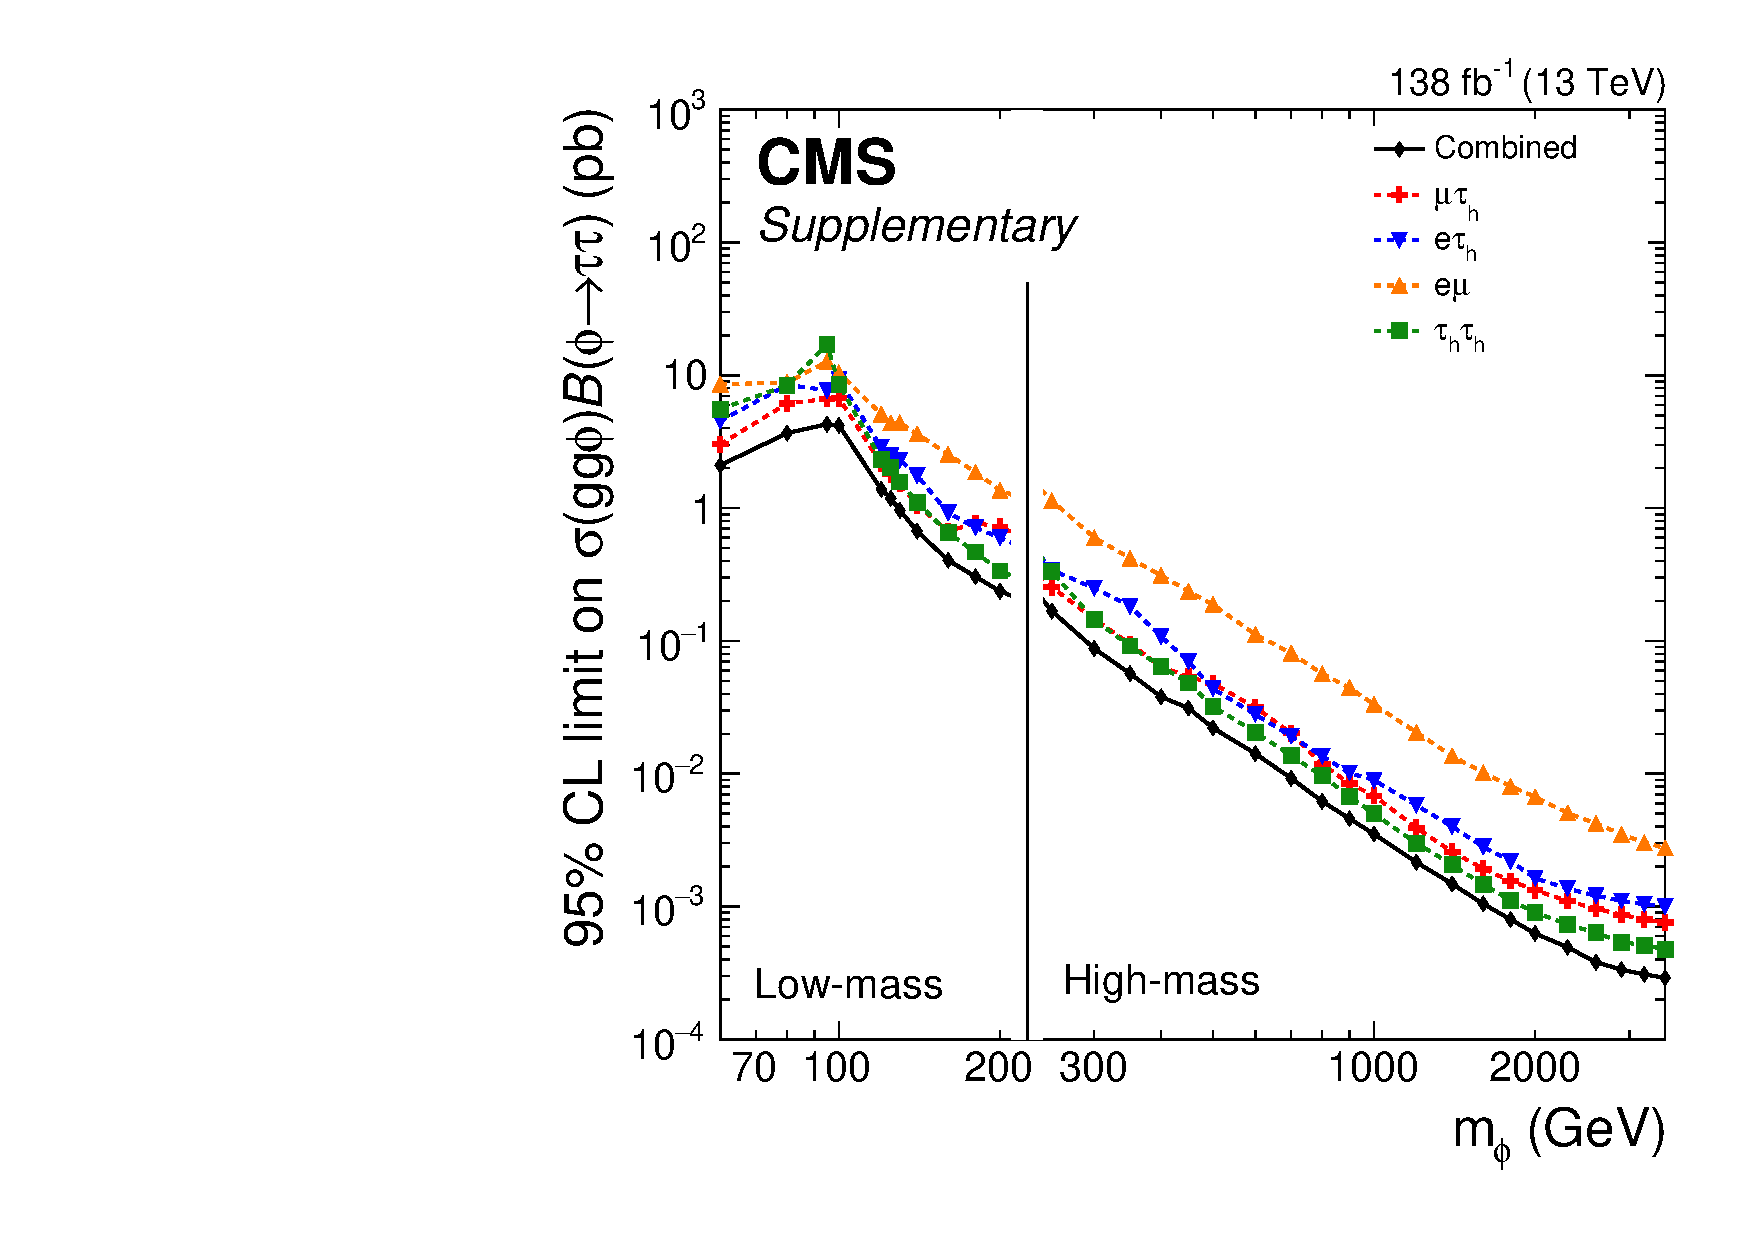
\includegraphics[width=0.5\textwidth]{Figures/limit_comparison_mssm_ggphi.pdf}}
    \subfloat[]{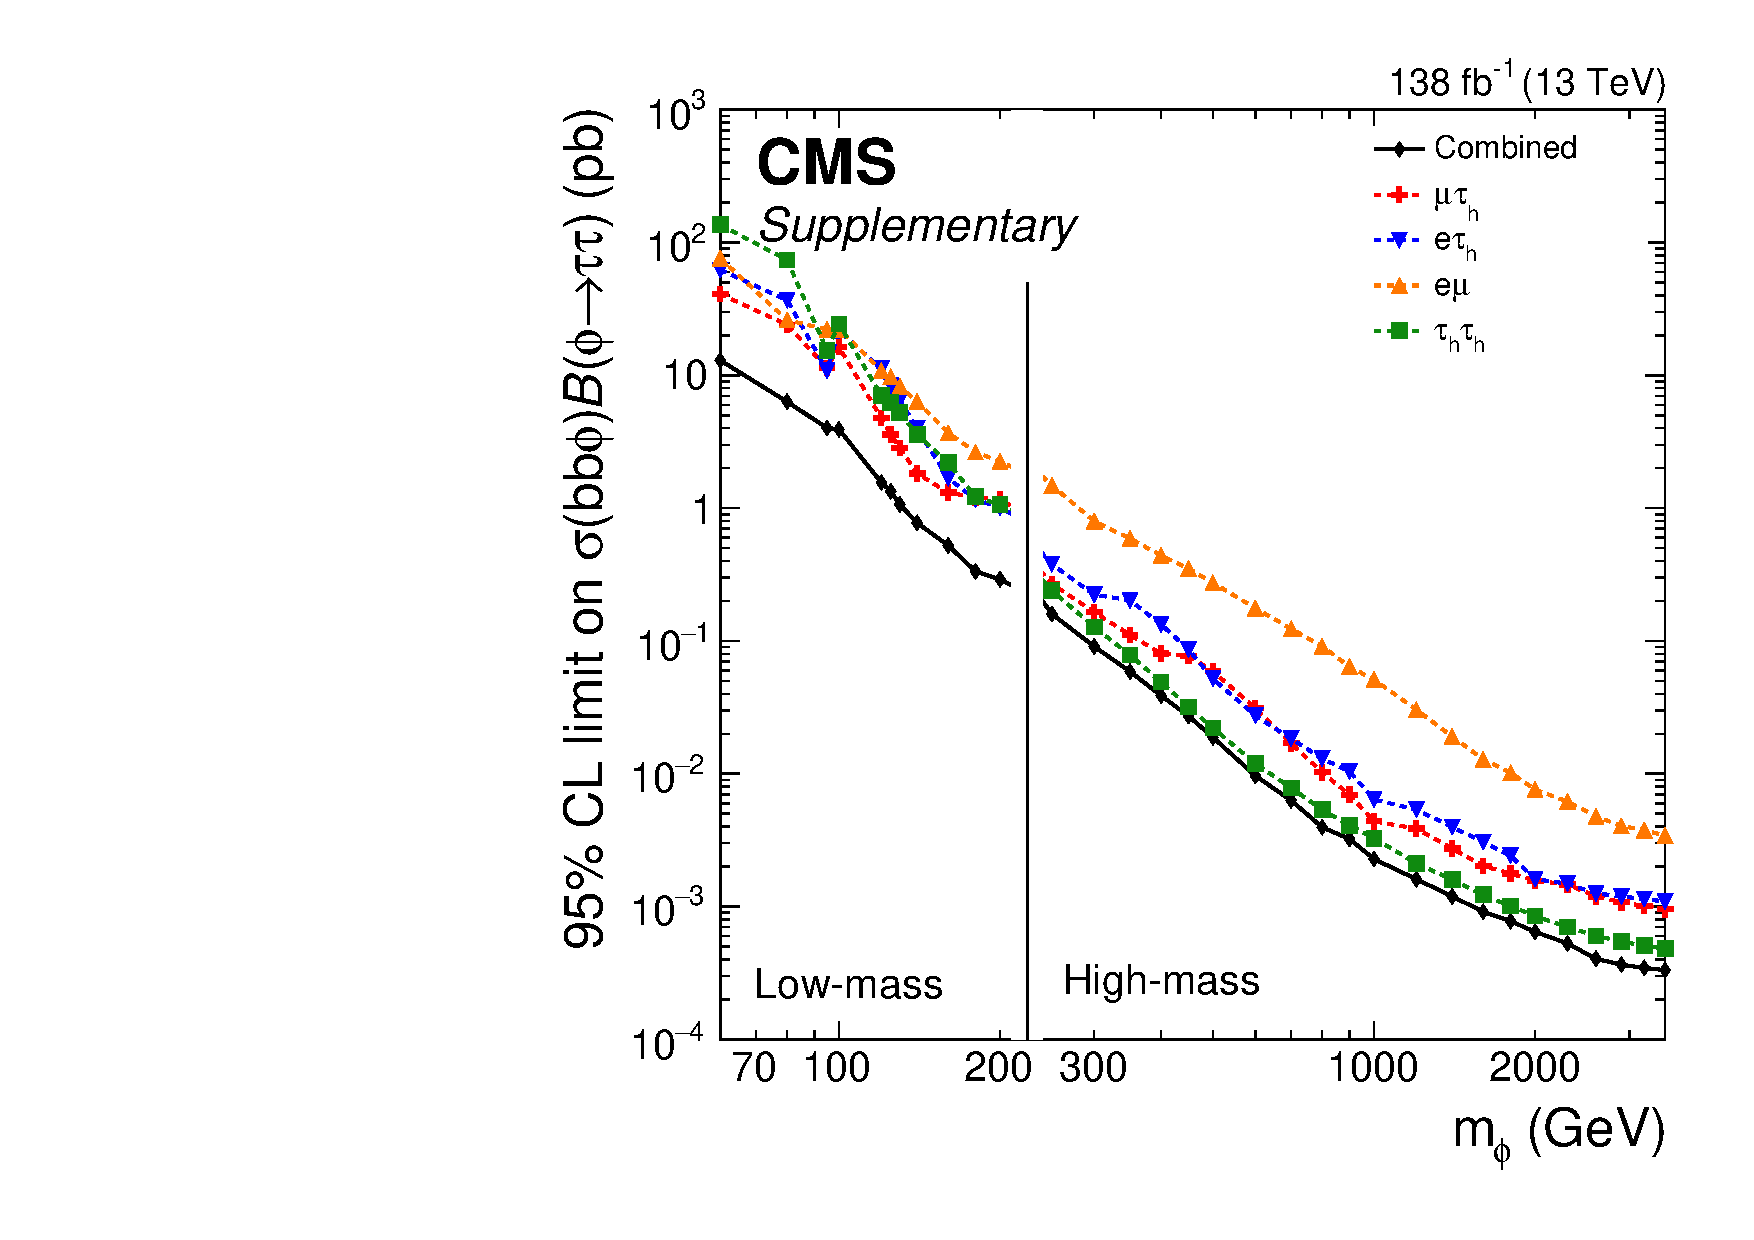
\includegraphics[width=0.5\textwidth]{Figures/limit_comparison_mssm_bbphi.pdf}}
\caption{Comparison of the expected 95\% CL upper limits on the product of the cross sections and branching fraction for the decay into $\tau$ leptons for (left) gg$\phi$ and (right) bb$\phi$ production, split by the $\tau\tau$ decay products fit individually.}
\label{fig:model_independent_limits_by_channel}
\end{figure}

A comparison of the limits are also made with the ATLAS experiment and in particular the results presented in Ref.~\cite{ATLAS:2020zms}.
This ATLAS search looks for the same signal but over a smaller mass range, from 200 GeV to 2.5 TeV.
Plots showing the comparison of the expected and observed limits for gg$\phi$ and bb$\phi$ are shown in Figure~\ref{fig:model_independent_limits_ATLAS}.
The expected limits from the CMS and ATLAS results are roughly compatible over the shared mass range, except at high mass where the extra statistics from the $Z\rightarrow \tau\tau$ samples compared to MC allow for lower background uncertainties and hence a stronger limit.
The ATLAS result observed no excess of events compatible with gg$\phi$ signal at 1.2 TeV, in fact a small deficit was observed.
Also, ATLAS observed local excesses at 400 GeV of 2.2$\sigma$ for gg$\phi$ and 2.7$\sigma$ for bb$\phi$.
None of these excesses are consistent between the ATLAS and CMS results.
The ATLAS search does not stretch to the mass of the low mass CMS excess and so cannot be used a cross-check for this.

\begin{figure}[!hbtp]
\centering
    \subfloat[]{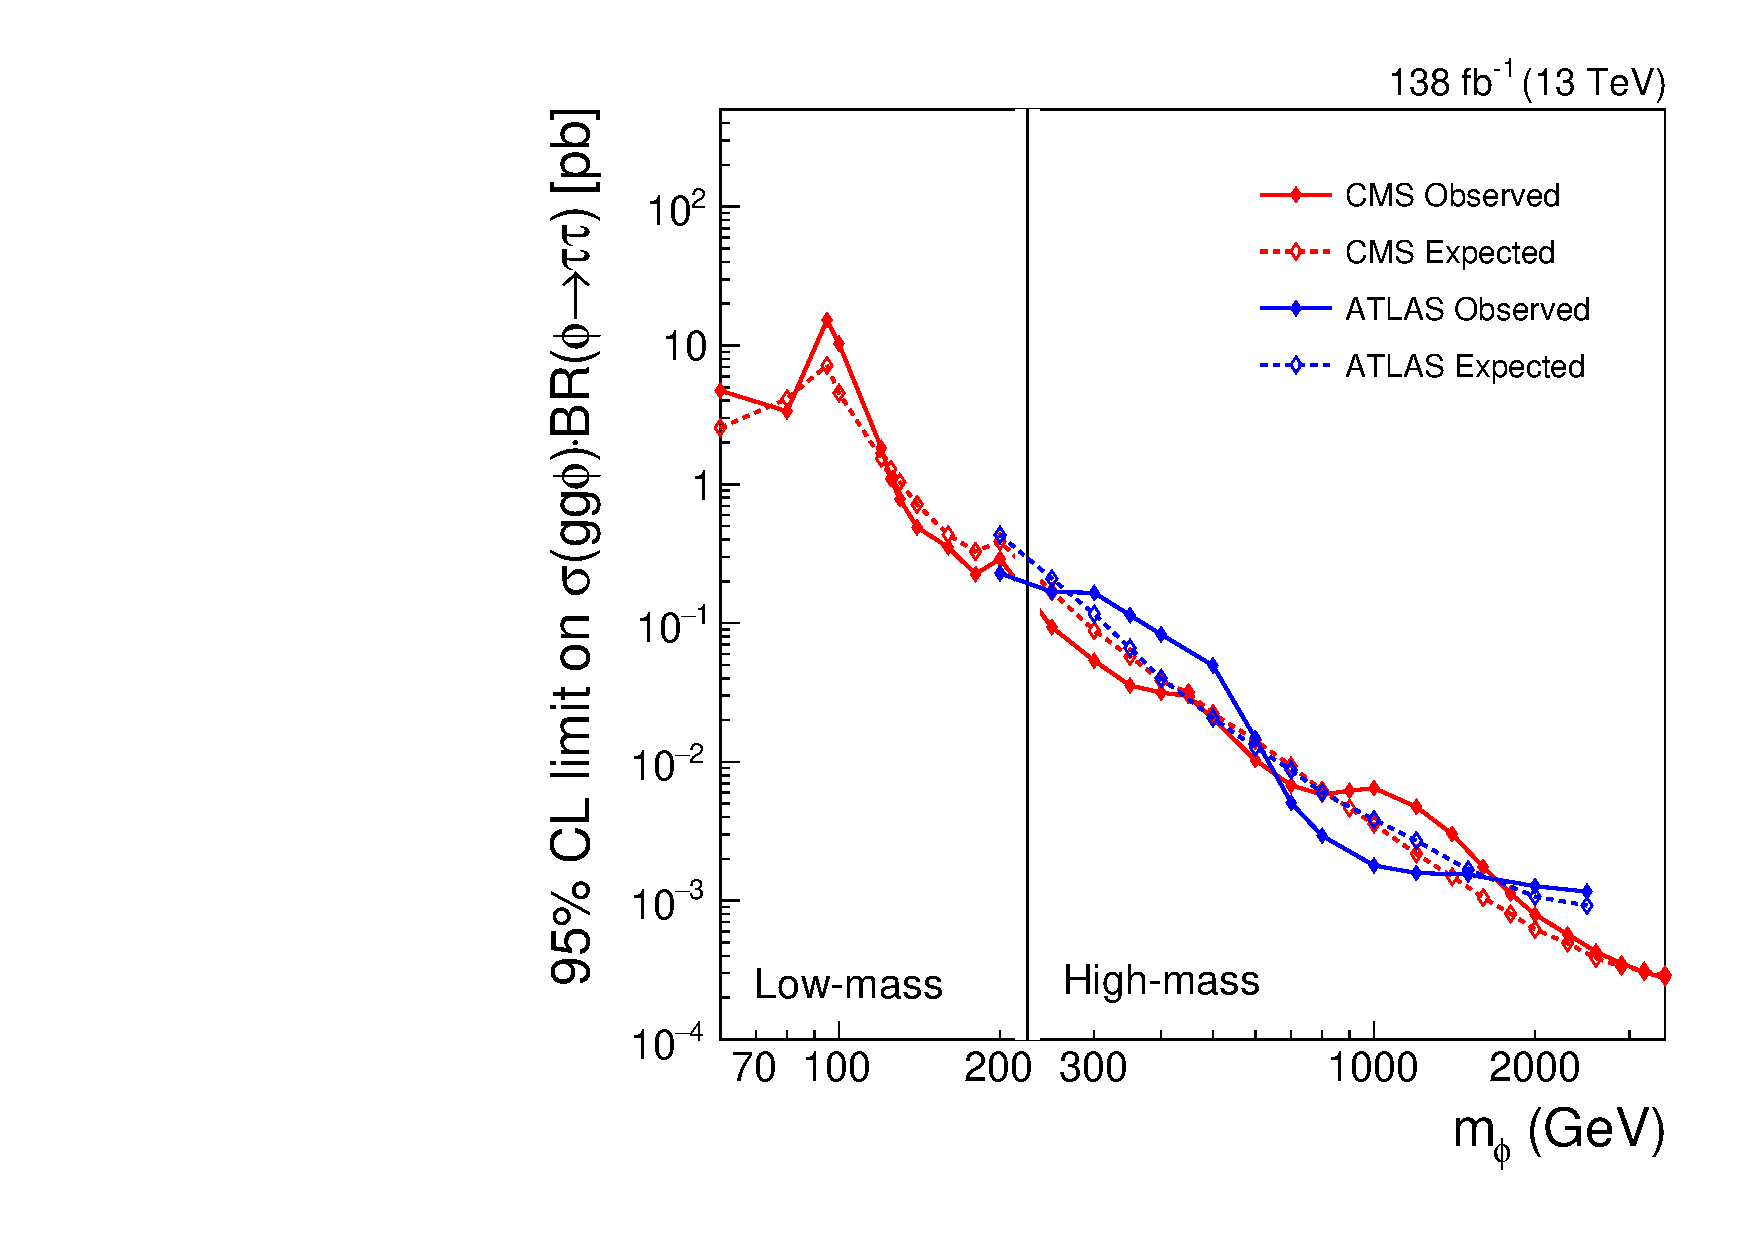
\includegraphics[width=0.5\textwidth]{Figures/limit_comparison_gg_ATLAS.pdf}}
    \subfloat[]{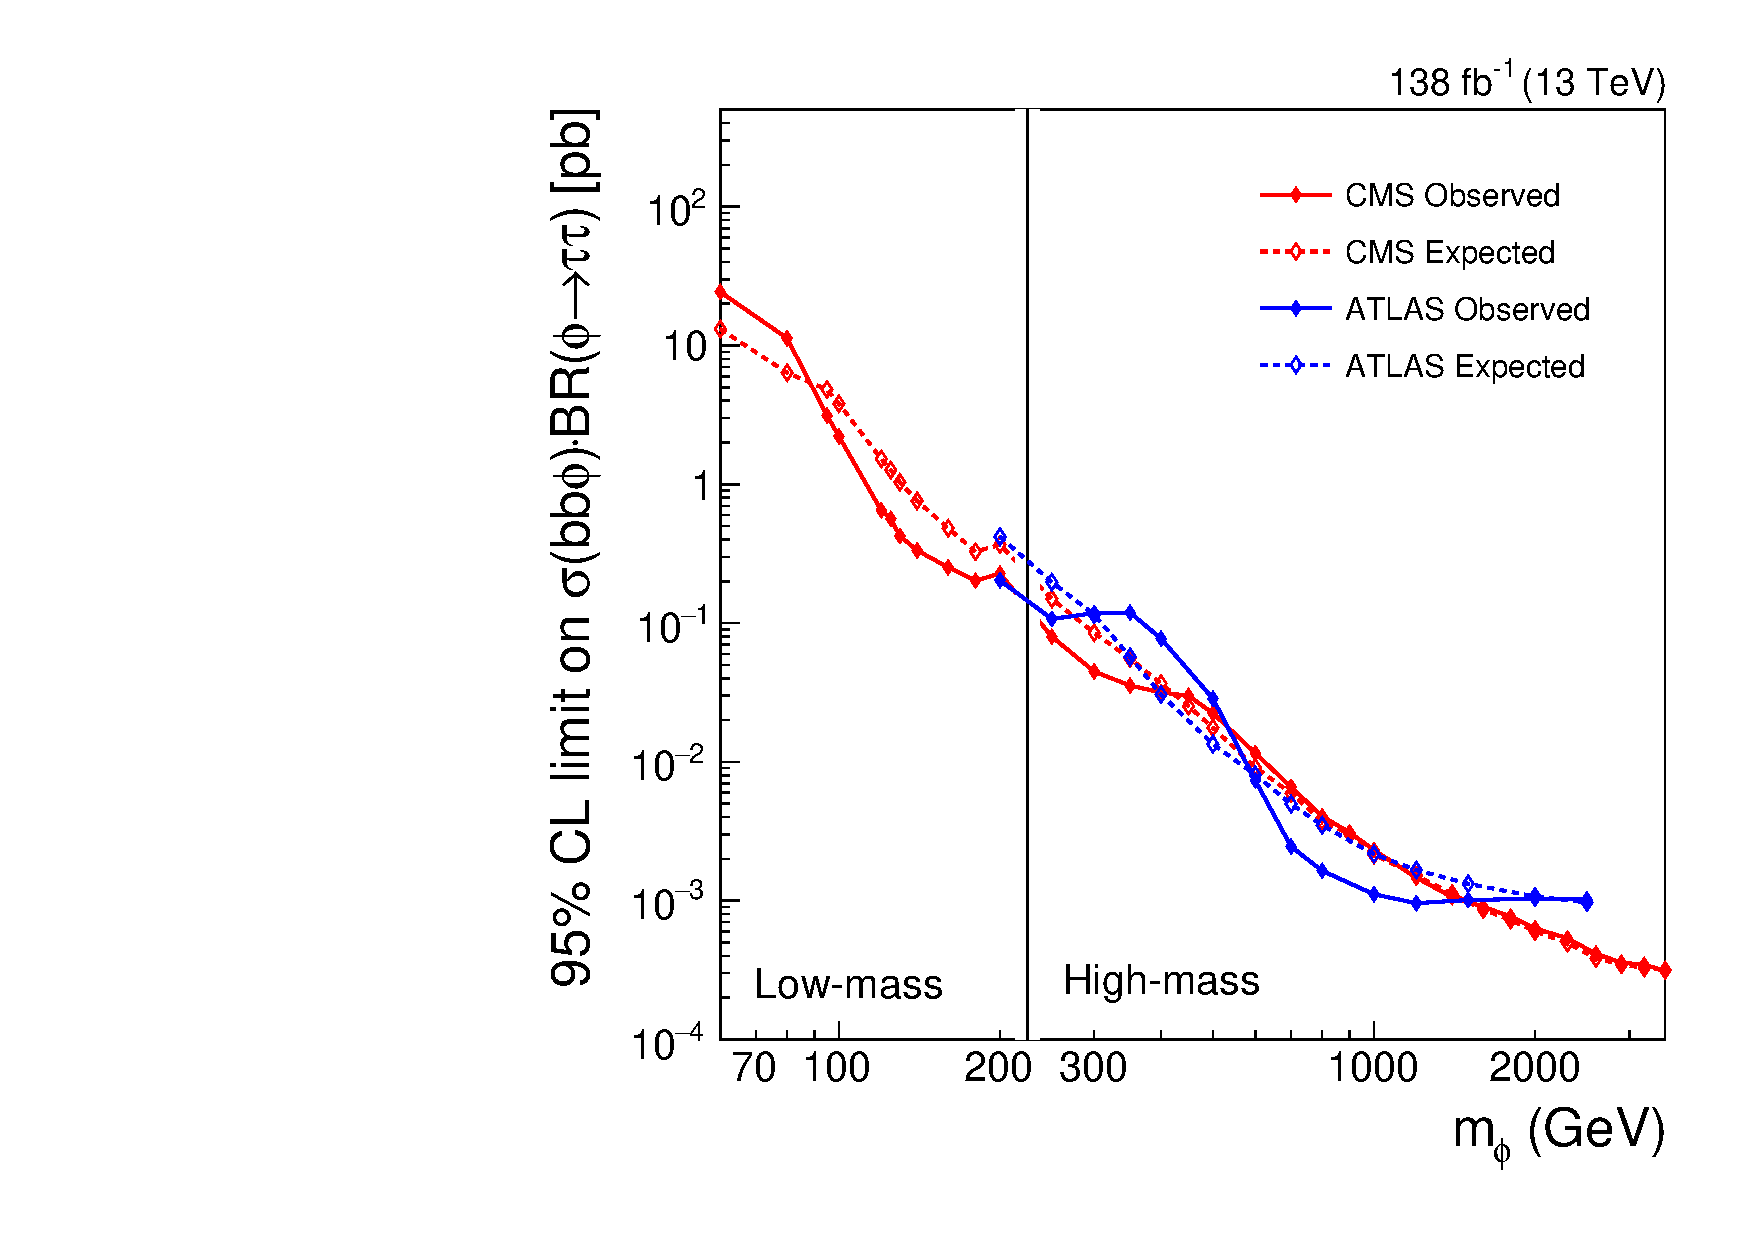
\includegraphics[width=0.5\textwidth]{Figures/limit_comparison_bb_ATLAS.pdf}}
\caption{Comparison of the expected 95\% CL upper limits on the product of the cross sections and branching fraction for the decay into $\tau$ leptons for (left) gg$\phi$ and (right) bb$\phi$ production, split by the CMS result detailed in this thesis and the ATLAS result from Ref.~\cite{ATLAS:2020zms}.}
\label{fig:model_independent_limits_ATLAS}
\end{figure}

\subsection{Significance and Compatibility}

The $p$-values and significances at each model independent signal hypothesis are calculated as described in Section~\ref{sec:sig_ext} and shown in Figure~\ref{fig:significance}.
Identical to the model independent limits, the gg$\phi$ or bb$\phi$ process is allowed to float freely if not the parameter of interest.
The excesses for the gg$\phi$ process peak at 100 GeV and 1.2 TeV and quantify to a local (global) significance of 3.1$\sigma$ (2.7$\sigma$) and 2.8$\sigma$ (2.2$\sigma$).
There are also excesses at neighbouring mass points (particularly at high mass), however this is consistent with the mass resolution of the fitted templates for the central values.
No deviations beyond 2$\sigma$ are observed for bb$\phi$ production.

\begin{figure}[!hbtp]
\centering
    \subfloat[]{\includegraphics[width=0.5\textwidth]{Figures/significance_plot_ggH.pdf}}
    \subfloat[]{\includegraphics[width=0.5\textwidth]{Figures/significance_plot_bbH.pdf}}
\caption{Local $p$-value and significance of a gg$\phi$ (left) and bb$\phi$ (right) signal as a function of $m_{\phi}$.}
\label{fig:significance}
\end{figure}

As many different decay channels and categories are used to extract these significances, the signal strength is studied in each channel and category.
This is done via compatibility fits as described in Section~\ref{sec:sig_ext}, where the signal strength parameter in each channel/category is decoupled.
No statistically significant differences are observed in the best fit signal strength in any decay channel or category fit and $p$-values between each channel or category fit are always above 0.05.
Figure~\ref{fig:low_mass_compatibility} shows the results of the compatibility fits in the low mass optimisation categories split by di-tau decay channels and $\pT$ bins fit and Figure~\ref{fig:high_mass_compatibility} shows the compatibility fits in the high mass optimisation categories split by di-tau decay channels.
The low mass signal strengths are no more dominant in any $\pT$ region than another.
In both low and high mass cases, the signal strengths are consistent across di-tau decay channels.
There is a small shift in the high mass $\emu$ categories to a negative signal strength, these categories have little to no sensitivity to this signal in comparison to others and a small deficit is observed in data, resulting in fits for a negative signal strength with a large uncertainty. 


\begin{figure}[!hbtp]
\centering
    \subfloat[]{\includegraphics[width=0.5\textwidth]{Figures/ChannelCompatibilityCheck_FitResults_mH100_channel.pdf}}
    \subfloat[]{\includegraphics[width=0.5\textwidth]{Figures/ChannelCompatibilityCheck_FitResults_mH100_cat.pdf}}
\caption{Compatibility plots of the low mass excess split into analysis channels (a) and categories (b). In each case the fitted signal strength is decoupled in the bin shown on the plot.}
\label{fig:low_mass_compatibility}
\end{figure}

\begin{figure}[!hbtp]
\centering
    \includegraphics[width=0.5\textwidth]{Figures/ccc_fit_result_mH1200_per-channel.pdf}
\caption{Compatibility plots of the high mass excess split by analysis channels. In each case the fitted signal strength is decoupled in each channel.}
\label{fig:high_mass_compatibility}
\end{figure}

\subsection{2D Likelihood Scans}

As the model independent search looks for 2 signal modes at each mass point, the results for both processes happening simultaneously are studied.
This is done in the form of 2D likelihood scans.
The best fit cross section times branching fractions of each process and the 95\% and 68\% confidence intervals are shown for a number of different mass scenarios in Figure~\ref{fig:2d_likelihood_scans}.
The SM prediction in all plots is at (0,0).
These results highlight how the excesses at 100 GeV and 1.2 TeV are dominated in the phase space in which gg$\phi$ and not bb$\phi$ signals are allowed.
In the 60 GeV example, there are smaller deviations in both gg$\phi$ and bb$\phi$ and so the SM background is over 2$\sigma$ away.
Otherwise, signal strengths are completely compatible with the background expectation.


\begin{figure}[!hbtp]
\centering
    \subfloat[]{\includegraphics[width=0.33\textwidth]{Figures/2d_lkld_60.pdf}}
    \subfloat[]{\includegraphics[width=0.33\textwidth]{Figures/2d_lkld_100.pdf}}
    \subfloat[]{\includegraphics[width=0.33\textwidth]{Figures/2d_lkld_125.pdf}} \\
    \subfloat[]{\includegraphics[width=0.33\textwidth]{Figures/2d_lkld_160.pdf}}
    \subfloat[]{\includegraphics[width=0.33\textwidth]{Figures/2d_lkld_250.pdf}}
    \subfloat[]{\includegraphics[width=0.33\textwidth]{Figures/2d_lkld_500.pdf}} \\
    \subfloat[]{\includegraphics[width=0.33\textwidth]{Figures/2d_lkld_1000.pdf}}
    \subfloat[]{\includegraphics[width=0.33\textwidth]{Figures/2d_lkld_1200.pdf}}
    \subfloat[]{\includegraphics[width=0.33\textwidth]{Figures/2d_lkld_3500.pdf}}
\caption{Maximum likelihood scans, including 68\% and 95\% CL contours obtained from the signal likelihood for the model-independent search. The scans are shown for selected values of $m_{\phi}$ between 60 GeV and 3.5 TeV.}
\label{fig:2d_likelihood_scans}
\end{figure}

\newpage
\section{Model Dependent Limits}

The exclusion contours for two benchmark scenarios of the MSSM, $M_{h}^{125}$ and $M_{h,EFT}^{125}$, are presented in Figure~\ref{fig:mssm_limits}. 
The red hatched regions denote areas where $m_{h}$ is inconsistent with the observed SM Higgs boson mass within a ${\pm}3$ GeV boundary. 
For low values of $\tan\beta$, higher values of the additional SUSY particle masses, denoted as $m_{\text{SUSY}}$, are needed to explain a mass of approximately $125$ GeV for the Higgs boson. 
In the $M_{h}^{125}$ scenario, $m_{\text{SUSY}}$ is fixed, and the predicted value of $m_{h}$ is below $122$ GeV. 
In contrast, the $M_{h,EFT}^{125}$ scenario adjusts $m_{\text{SUSY}}$ to satisfy the required value of $m_{h}$ for each point in ($m_{A}$, $\tan\beta$) individually, accounting for the logarithmic corrections associated with the large values of $m_{\text{SUSY}}$ using an effective field theory approach. 
The red hatched region in Figure~\ref{fig:mssm_limits} (b) indicates that the required values of $m_{\text{SUSY}}$ exceed the GUT scale at very low values of $m_{A}$ in this scenario. 
The Higgs boson masses, mixing angle $\alpha$, and effective Yukawa couplings were calculated using \textsc{FeynHiggs}, and branching fractions for the decay into tau leptons and other final states were obtained from a combination of the \textsc{FeynHiggs} and \textsc{HDECAY}, following the prescriptions in Refs.\cite{LHCHiggsCrossSectionWorkingGroup:2013rie,deFlorian:2016spz,Denner:2011mq}, for the scenarios described in Ref.\cite{Bagnaschi:2791954}. \\

For the $M_{h,EFT}^{125}$ scenario, the sensitivity sharply drops at $m_{A}=2m_{t}$ due to a drop in the branching fractions for the decay of A and H into tau leptons, when the A and H decays into two on-shell top quarks becomes kinematically accessible. 
Both scenarios are excluded at 95\% CL for $\mA\lesssim350$ GeV. 
For $\mA\lesssim250$ GeV, most of the ggH/A events do not enter the no b tag categories due to the $m_{\tau\tau}>250$ GeV requirement. 
In this parameter space, the sensitivity to the MSSM is driven by the measurements of the observed Higgs boson, even though H and A still contribute to the categories here. 
The sensitivity to the H and A enters mainly via the bb$\phi$ signal in the b tag categories, especially for increasing values of $\tan\beta$. \\

Other MSSM scenarios are tested and detailed in \cite{}.
One scenario of note is the $M_{H}^{125}$ scenario, which is the equivalent scenario to the $M_{h}^{125}$ but with the observed Higgs boson being the heavier CP-even Higgs boson.
Despite the local excess at a resonant mass of 100 GeV, this scenario is entirely excluded by the search. 
This is mostly due to the sensitivity of the b tag categories to b associated production.
The local excess observed at 1.2 TeV is hard to rectify within these MSSM benchmark scenarios.
The lack of any excess in the b tag categories strictly constrains the b associated production cross section times branching fraction.
It is not possible within these scenarios to predict the excess of gluon fusion events within the constraints placed on b associated production.

\begin{figure}[!hbtp]
\centering
    \subfloat[]{\includegraphics[width=0.65\textwidth]{Figures/model-dependent_limit_mh125.pdf}} \\
    \subfloat[]{\includegraphics[width=0.65\textwidth]{Figures/model-dependent_limit_mh125EFT.pdf}}
\caption{Expected and observed 95\% CL exclusion contours in the MSSM $M_{h}^{125}$ (a) and $M_{h,EFT}^{125}$ (b) scenarios. The exclusion limit only on background expectation is shown as a dashed black line, the dark and bright grey bands show the 68\% and 95\% intervals of the expected exclusion and the observed exclusion contour is shown by the blue area. The parameter space where \mh deviates by more then ${\pm}3$ GeV from the observed SM Higgs boson mass it shown by a red hatched area.
}
\label{fig:mssm_limits}
\end{figure}

Upper limits of 95\% confidence level for VLQ BM 1 and 2 are shown Figure~\ref{fig:vlq_limits}. 
These are drawn with respect to the leptoquark mass ($m_{U}$) and coupling ($g_{U}$).
The limit on $g_{U}$ decreases as $m_{U}$ increases, with values of $g_U$ ranging from 1.3 to 5.2 in VLQ BM 1 and 0.8 to 3.2 in VLQ BM 2. 
VLQ BM 2 has stronger exclusion limits than VLQ BM 1 due to additional right-handed couplings of the leptoquark with a bottom quark and a tau lepton.
The observed limits fall within the central 95\% intervals of the expected limits when no signal is present. 
The expected limits are also within the 95\% confidence interval of the best fit results reported by Ref.\cite{Cornella:2021sby}, indicating that the search is capable of detecting a part of the parameter space that can explain the anomalies observed in b physics. \\

Similarly to the MSSM scenarios, the local excess at 1.2 TeV is not consistent with a VLQ BM 1 or 2 vector leptoquark.
Again this is due to lack of signal in the b tag categories, where the reduction in backgrounds makes the t-channel signal with initial state radiation the dominant search option.

\begin{figure}[!hbtp]
\centering
    \subfloat[]{\includegraphics[width=0.65\textwidth]{Figures/vlq_bm_1.pdf}} \\
    \subfloat[]{\includegraphics[width=0.65\textwidth]{Figures/vlq_bm_2.pdf}}
\caption{Expected and observed 95\% CL upper limits on \gU in the VLQ BM 1 (a) and 2 (b) scenarios, in a mass range of $1<m_{U}<5$ TeV.  The exclusion limit only on background expectation is shown as a dashed black line, the dark and bright grey bands show the 68\% and 95\% intervals of the expected exclusion and the observed exclusion contour is shown by the blue area. The 95\% confidence interval for the preferred region from the global fit presented in Ref.~\cite{Cornella:2021sby} is also shown by the green shaded area.
}
\label{fig:vlq_limits}
\end{figure}

